\documentclass[fleqn,11pt,openany]{book}

% These two need to be set before including scirun style package
\title{SCIRun Forward/Inverse ECG Toolkit}
\author{Jaume Coll-Font, Moritz Dannhauer, Michael Steffen, Darrell Swenson, Dafang Wang, Burak Erem, Jess Tate, Jeroen Stinstra, Dana Brooks and Rob MacLeod}

% INCLUDE SCI STYLE DOCUMENT
\usepackage{scirun}
\usepackage{graphicx}
\usepackage{float}

% This makes displaying bold greek letters easier
\newcommand{\BM }[1]{\mbox{\boldmath $#1$}}

\begin{document}

%% starting from SCIRun Doc wiki


% CREATE TITLE PAGE --------------------------------------------------
\maketitle

% CHAPTERS ---------------------------------------------------------------

%\chapter{Overview}

\begin{introduction}

This guide describes and documents the SCIRun ECG Forward/Inverse
Toolkit. This toolkit is a collection of modules and networks
within the SCIRun system, which can be used to solve forward and inverse
electrocardiography problems. The guide assumes that the reader has basic
user-level familiarity with SCIRun; in particular that the reader is
familiar with placing modules into a SCIRun network, connecting modules,
and visualizing data. If the reader is not familiar with these operations,
we suggest you first consult the SCIRun Basic Tutorial, also distributed in
the SCIRun documentation.

The purpose of this toolkit is to advance the state of forward and inverse
solutions in this field by offering a common platform for investigators and
others to compare geometries and geometric representations, forward and inverse algorithms and data, with the maximum degree of both flexibility
and commonality that we can achieve. Thus, we hope to increase the
"reproducibility'' of developments in this field and help
move these technologies closer to useful clinical applications. As such, the
software (like all of SCIRun) is open-source, modular, and extensible. We
follow modern open-source software engineering practices to maximize
portability, extensibility, and reliability of our software. As we explain below, SCIRun has a
built-in facility for connecting with Python, or Matlab through Python, so that processing can be
carried out jointly using both programs. In
addition, the ECG Forward/Inverse Toolkit features capabilities which allow
the user to interface with ECGSim (\href{http://www.ecgsim.org}{http://www.ecgsim.org}), a
popular software package for solving certain types of forward ECG problems
with a high degree of interactive control over source models).

We welcome inquiries from users about this toolkit, and very much encourage
contributions to the toolkit from the community. For more information
about the toolkit or the underlying algorithms, or to discuss contributing to
its development, please contact \textit{scirun-users@sci.utah.edu}.

This toolkit is a product of the Center for Integrative Biomedical
Computing (CIBC), an NIH supported Biomedical Technology Research Center,
and we gratefully acknowledge the support from NIH that has made the
development of this work possible. The CIBC is housed in the Scientific
Computing and Imaging (SCI) Institute at the University of Utah and the
environment and personnel in SCI have also been integral to the development of the toolkit.

\end{introduction}

\section{Toolkit overview and capabilities}

Computational modeling of bioelectric fields often requires the solution of
electrocardiographic or electroencephalographic forward and inverse
problems in order to non-invasively analyze electrophysiological events
that are otherwise inaccessible or unethical to explore. All solutions to
both problems require a common set of components, each of which is then
customized or optimized for the particular problem formulation.
Bioelectric activity begins from a biophysical source of voltage or current,
which for computational purposes must be modeled in an appropriate,
problem-specific form. For example, when the clinical mission is to
identify focal activation in the brain, one or more current dipoles may be
a suitable source model. However, when the goal is to reconstruct the
sequence of activation across the ventricles of the heart, the sources are
better modeled in more complex form to capture the wavefront of this
activation. Each type of source then requires an approximation in
mathematical and then numerical form. Such a source model can then be used
(in a solution to the \textit{forward} problem) to computationally generate
the associated voltages on the surface of the body (or wherever
measurements might be made). If the goal is to recover sources from
measured potentials, \textit{i.e.} to solve the \textit{inverse} problem,
such as in the activation sequence reconstruction just mentioned, the
solution strategy must include appropriate numerical techniques that can
incorporate constraints and recover useful solutions, even when the inverse
problem is poorly posed and hence the forward problem numerically ill-conditioned.

Creating complete software solutions to such problems from scratch is a
daunting undertaking, requiring both considerable resources and considerable
breadth of expertise. It is in order to make such tools more accessible to
a broader array of researchers, and to enable validation and comparison
across solution approaches, that the Center for Integrative Biomedical
Computing (CIBC) has created this ECG Forward/Inverse toolkit. It is
designed to provide a generalized software environment, based on the open-source
SCIRun system, to aid researchers to construct, execute, visualize,
and compare such computational models.

SCIRun is based on a data flow-visual programming paradigm, in which distinct
computational (and software) modules are linked by connections (``data
pipes'') to form functional networks. The network editor offers the user
interactive control and flexibility to assemble the specific network needed to
solve the computational task at hand.
The ECG Forward/Inverse toolkit provides
a diverse array of modules, with associated data types, for bioelectric field problems,
together with sample networks and data sets with which to explore its
functionality.
An additional key feature of using the SCIRun system is
that rather than requiring custom code for all its functionality, the
toolkit leverages SCIRun's ability to
connect directly to Matlab through a
bi-directional Matlab interface, and has capabilities to read in data
created by ECGSim, as mentioned above.

Table \ref{tab:prop} lists currently available forward and inverse
approaches explicitly provided within the toolkit. The toolkit contains
full simulation example networks that illustrate potential and
activation-based forward models using both finite element (FEM) and boundary
element (BEM) approximation techniques as well as selected potential and
activation-based inverse methods. As indicated by the table,
simulation specific tools, such as lead field and stiffness matrix
generators, as well as a variety of regularization modules, are also
included, and can easily be included in user-built networks.

\begin{table}[htb]
\begin{tabular}{|ll|l|}
\hline
{\bf Forward tools} & {\bf Inverse Tools}\\ \hline
\hline
Potential-Based FEM/BEM & Activation-Based$^{\&}$$^{*}$\\ \hline
Activation-Based FEM$^{\dag}$ & Potential-Based Regularization  Methods\\ \hline
FEM Lead Field Calculation &   -  Tikhonov  \\ \hline
Stiffness Matrix Calculation &- Tikhonov SVD  \\ \hline
 & - Truncated SVD\\ \hline
 & - Isotropy method$^{*}$\\ \hline
 & - Gauss-Newton Method$^{*}$\\ \hline
 & - Wavefront based potential reconstruction$^*$\\ \hline
 & - Total Variation \\ \hline
\end{tabular}
\caption{Algorithms currently included in the CIBC ECG Forward/Inverse
toolkit \newline
$^\dag$Activation-based BEM forward solution is currently
unavailable in the toolkit \newline
$^{\&}$Based on a Gauss-Newton optimization \newline
$^{*}$Requires Matlab
}
\label{tab:prop}
\end{table}

\newpage

\section{Software requirements}

\subsection{SCIRun Compatibility}

The modules demonstrated in this tutorial are available in SCIRun
version 4.5 and higher. This tutorial is not compatible with earlier
 versions of SCIRun. If you have an existing SCIRun installation, we
 strongly encourage you to update your SCIRun version
to the latest build, available from the SCI software portal
(\href{http://software.sci.utah.edu}{http://software.sci.utah.edu}), which will include the latest bug
fixes and ensure that your version is up to date with the capabilities demonstrated in this guide.

\subsection{Required Datasets}

This tutorial relies on several datasets that are freely distributed as part of the
SCIRunData bundle. To obtain these datasets, please go to the SCI
software portal at \newline\href{http://software.sci.utah.edu}{http://software.sci.utah.edu} and click on {\bf
Download SCIRun} to download the SCIRunData zip files. The SCIRunData
dataset is provided in both zip and gzip file formats for your convenience.


% Overview ---------------------------------------------------------------
\chapter{Overview}

\begin{introduction}

This guide describes and documents the SCIRun ECG Forward/Inverse
Toolkit. This toolkit is a collection of modules and networks
within the SCIRun system, which can be used to solve forward and inverse
electrocardiography problems. The guide assumes that the reader has basic
user-level familiarity with SCIRun; in particular that the reader is
familiar with placing modules into a SCIRun network, connecting modules,
and visualizing data. If the reader is not familiar with these operations,
we suggest you first consult the SCIRun Basic Tutorial, also distributed in
the SCIRun documentation.

The purpose of this toolkit is to advance the state of forward and inverse
solutions in this field by offering a common platform for investigators and
others to compare geometries and geometric representations, forward and inverse algorithms and data, with the maximum degree of both flexibility
and commonality that we can achieve. Thus, we hope to increase the
"reproducibility'' of developments in this field and help
move these technologies closer to useful clinical applications. As such, the
software (like all of SCIRun) is open-source, modular, and extensible. We
follow modern open-source software engineering practices to maximize
portability, extensibility, and reliability of our software. As we explain below, SCIRun has a
built-in facility for connecting with Matlab so that processing can be
carried out jointly using both programs. In
addition, the ECG Forward/Inverse Toolkit features capabilities which allow
the user to interface with ECGSim (\href{http://www.ecgsim.org}{http://www.ecgsim.org}), a
popular software package for solving certain types of forward ECG problems
with a high degree of interactive control over source models).

We welcome inquiries from users about this toolkit, and very much encourage
contributions to the toolkit from the community. For more information
about the toolkit or the underlying algorithms, or to discuss contributing to
its development, please contact \textit{scirun-users@sci.utah.edu}.

This toolkit is a product of the Center for Integrative Biomedical
Computing (CIBC), an NIH supported Biomedical Technology Research Center,
and we gratefully acknowledge the support from NIH that has made the
development of this work possible. The CIBC is housed in the Scientific
Computing and Imaging (SCI) Institute at the University of Utah and the
environment and personnel in SCI have also been integral to the development of the toolkit.

\end{introduction}

\section{Toolkit overview and capabilities}

Computational modeling of bioelectric fields often requires the solution of
electrocardiographic or electroencephalographic forward and inverse
problems in order to non-invasively analyze electrophysiological events
that are otherwise inaccessible or unethical to explore. All solutions to
both problems require a common set of components, each of which is then
customized or optimized for the particular problem formulation.
Bioelectric activity begins from a biophysical source of voltage or current,
which for computational purposes must be modeled in an appropriate,
problem-specific form. For example, when the clinical mission is to
identify focal activation in the brain, one or more current dipoles may be
a suitable source model. However, when the goal is to reconstruct the
sequence of activation across the ventricles of the heart, the sources are
better modeled in more complex form to capture the wavefront of this
activation. Each type of source then requires an approximation in
mathematical and then numerical form. Such a source model can then be used
(in a solution to the \textit{forward} problem) to computationally generate
the associated voltages on the surface of the body (or wherever
measurements might be made). If the goal is to recover sources from
measured potentials, \textit{i.e.} to solve the \textit{inverse} problem,
such as in the activation sequence reconstruction just mentioned, the
solution strategy must include appropriate numerical techniques that can
incorporate constraints and recover useful solutions, even when the inverse
problem is poorly posed and hence the forward problem numerically ill-conditioned.

Creating complete software solutions to such problems from scratch is a
daunting undertaking, requiring both considerable resources and considerable
breadth of expertise. It is in order to make such tools more accessible to
a broader array of researchers, and to enable validation and comparison
across solution approaches, that the Center for Integrative Biomedical
Computing (CIBC) has created this ECG Forward/Inverse toolkit. It is
designed to provide a generalized software environment, based on the open-source
SCIRun system, to aid researchers to construct, execute, visualize,
and compare such computational models.

SCIRun is based on a data flow-visual programming paradigm, in which distinct
computational (and software) modules are linked by connections (``data
pipes'') to form functional networks. The network editor offers the user
interactive control and flexibility to assemble the specific network needed to
solve the computational task at hand.
The ECG Forward/Inverse toolkit provides
a diverse array of modules, with associated data types, for bioelectric field problems,
together with sample networks and data sets with which to explore its
functionality.
An additional key feature of using the SCIRun system is
that rather than requiring custom code for all its functionality, the
toolkit leverages SCIRun's ability to
connect directly to Matlab through a
bi-directional Matlab interface, and has capabilities to read in data
created by ECGSim, as mentioned above.

Table \ref{tab:prop} lists currently available forward and inverse
approaches explicitly provided within the toolkit. The toolkit contains
full simulation example networks that illustrate potential and
activation-based forward models using both finite element (FEM) and boundary
element (BEM) approximation techniques as well as selected potential and
activation-based inverse methods. As indicated by the table,
simulation specific tools, such as lead field and stiffness matrix
generators, as well as a variety of regularization modules, are also
included, and can easily be included in user-built networks.

\begin{table}[htb]
\begin{tabular}{|ll|l|}
\hline
{\bf Forward tools} & {\bf Inverse Tools}\\ \hline
\hline
Potential-Based FEM/BEM & Activation-Based$^{\&}$$^{*}$\\ \hline
Activation-Based FEM$^{\dag}$ & Potential-Based Regularization  Methods\\ \hline
FEM Lead Field Calculation &   -  Tikhonov  \\ \hline
Stiffness Matrix Calculation &- Tikhonov SVD  \\ \hline
 & - Truncated SVD\\ \hline
 & - Isotropy method$^{*}$\\ \hline
 & - Gauss-Newton Method$^{*}$\\ \hline
 & - Wavefront based potential reconstruction$^*$\\ \hline
 & - Total Variation \\ \hline
\end{tabular}
\caption{Algorithms currently included in the CIBC ECG Forward/Inverse
toolkit \newline
$^\dag$Activation-based BEM forward solution is currently
unavailable in the toolkit \newline
$^{\&}$Based on a Gauss-Newton optimization \newline
$^{*}$Requires Matlab
}
\label{tab:prop}
\end{table}

\newpage

\section{Software requirements}

\subsection{SCIRun Compatibility}

The modules demonstrated in this tutorial are available in SCIRun
version 4.5 and higher. This tutorial is not compatible with earlier
 versions of SCIRun. If you have an existing SCIRun installation, we
 strongly encourage you to update your SCIRun version
to the latest build, available from the SCI software portal
(\href{http://software.sci.utah.edu}{http://software.sci.utah.edu}), which will include the latest bug
fixes and ensure that your version is up to date with the capabilities demonstrated in this guide.

\subsection{Required Datasets}

This tutorial relies on several datasets that are freely distributed as part of the
SCIRunData bundle. To obtain these datasets, please go to the SCI
software portal at \newline\href{http://software.sci.utah.edu}{http://software.sci.utah.edu} and click on {\bf
Download SCIRun} to download the SCIRunData zip files. The SCIRunData
dataset is provided in both zip and gzip file formats for your convenience.

% Math ---------------------------------------------------------------
%\chapter{Mathematical Background} \label{sec:math}

\section{Overview}

In this chapter we describe the basic mathematical formulations and some
solution approaches to the forward and inverse problems of
electrocardiography. The goal of solutions to the forward problem, also called ECG
forward Simulation, is to
predict potentials that could be measured in any accessible location
(usually the surface of the torso) given a description of the cardiac
electrical sources as well as the geometry and conductivities of the torso involved.
The goal of solutions to the inverse problem, also called ECG imaging or ECGI,
is to predict cardiac sources given a set
of measurements and the same geometry and conductivity information. It is
important to note that a solution to ECG Imaging presupposes an
available solution to the forward simulation.
Here we briefly summarize the basic background to
facilitate our description of the toolkit capabilities in subsequent chapters.
Please refer to the list of literature on the CEI webpage
for more information (\url{http://www.ecg-imaging.org/home/publications}).


Solving both forward and inverse problems requires a specific model formulation of
the cardiac electrical sources. This toolkit contains examples from the two arguably
most dominant equivalent source models used in current forward and inverse
problem research. One model, which we will refer to as the ``activation-based''
source model, assumes that the dominant feature of cardiac electrical activity
is the timing of the arrival of the depolarization wavefront (known as ``activation times'')
at each location in the heart. (A similar problem, in which the equivalent
sources called ''recovery times'' are the timing of repolarization at each
location, is solved in a similar fashion.) Classical results have shown that,
under assumptions of isotropy and homogeneity of
the myocardium, activation-based models can be reduced to the activation
times on the surface of the heart \cite{RSM:Oos2004}. In this context, this is usually taken as
the epicardial (outer) and endocardial (inner) heart surfaces, connected
across the base of the heart by an imaginary connecting surface. The source
in this case can be modeled by a moving set of current dipoles aligned
along the ``activation wavefront''; that is, the curve where activation is
taking place on this surface at any given time.

The second source model treated here, which we will refer to as the
``potential-based'' source model, assumes that the cardiac sources can be
represented by the time-varying electrical potentials present on a surface,
enclosing all the electrical sources. Gauss' Law implies that any such set
of potentials is unique, and that the closer the surface is to the myocardial
surface the more useful the model is. So, the surface is typically taken as
the epicardium, closed off by an imaginary ``top'' surface at the base of
the heart or, alternatively, the same joint epicardial/endocardial surface
used for activation-based models.

In the rest of this chapter we describe solutions to the forward and
inverse problem concentrating on the specific tools currently provided in
this toolkit. Again we refer the reader to the literature for more complete
background.

%%:
%%:
%%: The
%%: relationship of the torso potentials and heart source in generally
%%: expressed as $y=A(x)$ with $y$ as the torso potential vector, $x$ as the
%%: heart sources, and $A$ as the function that relates the torso surface to
%%: the heart surface. In this chapter, we will provide examples of different
%%: ways to formulate and compute the function $A$ and the torso potentials
%%: from heart sources using SCIRun.
%%:
%%: There are mainly two types of heart sources used in the forward problem:
%%: cardiac surface potentials, and activation times. The potential based
%%: forward problem is more intuitive and can be thought of as a projection of
%%: the cardiac potentials through the torso volume to the surface. Each point
%%: on the heart surface contributes directly to the torso surface potential in
%%: a way described by the transfer function $A$.  In this case of the
%%: potential-based forward problem, $A$ is a matrix, and the forward problem
%%: is solve by a matrix multiplication: $y=A \cdot x$, $x$ being the cardiac
%%: potential vector. The activation-time base-forward model is based on the
%%: concept that activation wavefront of the myocardium contains a high
%%: potential gradient with the rest of the heart either activated or resting,
%%: generating a current source along the wavefront. Using a uniform dipole
%%: layer to represent the source of the wavefront, one can calculate the torso
%%: surface potentials.
%%:
\section{Solutions to the Forward Problem in the Forward/Inverse Toolkit}

The temporal frequencies which are relevant to electrocardiographic
bioelectricity are relatively low, and the wavelengths many orders of
magnitude larger than the dimensions of the human body. So, from a
bioelectricity viewpoint, the governing partial differential equation (PDE)
is Laplace's equation:

\begin{equation} \nabla \cdot (\BM{\sigma} \nabla \Phi) = 0, \label{eq:eq}
\end{equation}
\noindent where $\BM{\sigma}$ contain the relevant conductivities and $\Phi$ the
electrical potentials. The boundary conditions are given by:
\begin{align} \Phi(x,y,z)|_{\Omega_k} &= V_k\\ \left. \frac{\partial
\Phi}{\partial \hat{n}} \right|_\Omega &= 0 \label{eq:bc}
\end{align}
\noindent where $\Omega_{k}$ is the surface on which the sources are located,
$V_k$ are the potentials on that surface, and $\hat{n}$ are the surface normals
of the surface.

As an alternative to solving this problem directly, a (weighted) integral
can be taken over the solution domain on both sides of Eq.~(\ref{eq:eq})
and the resulting integral equation solved for $\Phi$ at locations of
interest. This is usually referred to as the ``weak form'' of the PDE
solution, and (aside from discontinuities which theoretically could be
possible in the weak form solution but are not of practical importance
here) is equivalent to solving the original, or ``strong'' form.

In a tractable geometry, such as a set of concentric or even eccentric
spheres, this PDE can be solved via analytical expansions. However in
complex geometries such as realistic torso models, numerical solutions must
be applied.
%Again there is a large literature on such numerical methods.
Two of these methods have predominated in the literature for
forward electrocardiography: the Finite Element Method (FEM) and the
Boundary Element Method (BEM). It is these two methods which have been
implemented in this toolkit. Thus, in the rest of this subsection, we give a
very brief description of these two methods.

The major difference between FEM and BEM, from the practical application point of view,
is in the way in which they discretize the solution domain.
FEM relies on a volume discretization. The geometry of the solution domain
is describe by a mesh of small three dimensional volume elements,
each with its own conductivity parameters.
BEM, on the other hand, is a surface discretization
method, with the geometry represented as a collection of bounding surfaces
separating regions in the volume with different conductivities. Each of
these surfaces is then discretized into a mesh. In other words, in both FEM
and BEM there exists a collection of points, called nodes, which define the
respective volume or surface elements. The potential $\Phi$ (and the
current, $\BM{\sigma} \nabla \Phi)$, is approximated by interpolating the
potential and current across those elements based on its value at the
nodes using known (usually polynomial) interpolation functions. Thus,
numerical integration can be applied to the weak form, and the node values
come out of the integrals, leaving subintegrals over known functions which
result in a set of weights. The result in either case is a system of
linear equations.

The boundary conditions in Eq.~(\ref{eq:bc}) are applied differently  in FEM
and BEM, another important difference between the two methods.


%%:
%%: %%: collection of at surface elements. However, the BEM method is a
%%: global method in that all points ``see'' each other, resulting in a
%%: dense-matrix formulation while the basis functions used in FEM have
%%: compact support, resulting in a sparse-matrix formulation.
%%:

We note that either BEM or FEM can be applied to both activation-based and
potential-based source models, although there are important implementation
details. We briefly note these differences here, and some specifics of the
applications in the context of the relevant SCIRun modules will be
presented in Ch.~\ref{ch:fwd}.


%%: The inverse problem of electrocardiography is to invert the model in the forward problem or, in other words, to solve for sources on the heart that suitably fit the given body surface potentials and forward model. This forward relationship can be described by the equation $y=A(x)$ where $y$ is the vector of body surface potentials, $A$ is the forward function, and $x$ are the sources on the heart.
%%:
%%: Inverse solution methods can be split into two categories based on their source models: activation-based and potential-based. Potential-based source formulations typically assume that the sources are parameterized by electric potentials themselves and the forward function is linear matrix multiplication: $y=Ax$. Activation-based source formulations...
%%:

\subsection{FEM in the Forward/Inverse Toolkit}


%%: The Finite Element Method is a volume-discretization method and is
%%therefore a good choice when either the solution is desired throughout
%%the entire volume or when there are detailed volume-varying parameters,
%%such as conductivity, that are to be accounted for. FEM is fairly complex
%%and volumes of literature exist on the method. Below is a brief overview
%%of some of the key points of the method.
%%:

%%: As was previously stated, the steady state electrical potential in an
%%: inhomogeneous volume conductor is described by the equation
%%: %
%%: \begin{equation} \nabla \cdot (\BM{\sigma} \nabla \Phi) =
%%: 0, \label{eq:eq}.
%%: \end{equation}
%%: %
%%: and again, the boundary conditions are given by:
%%: \begin{align} \Phi(x,y,z)|_{\Omega_k} &= V_k\\ \left. \frac{\partial
%%: \Phi}{\partial n} \right|_\Omega &= 0.
%%: \end{align}
%%:
%%:

The finite element method begins by subdividing the geometry into a set of
volume elements with vertices at a set of nodes, and then approximating
the potential in the volume by a basis expansion:
\begin{equation} \bar{\Phi}(x,y,z) = \sum_i \Phi_i
N_i(x,y,z), \label{eq:approx}
\end{equation}
\noindent where $\{N_i\}$ are a set of basis functions, one for each node in the
volume element discretization, and
$\{\Phi_i\}$ are the corresponding (unknown) coefficients at those nodes.
Note that if the
$\{\Phi_i\}$ can be determined, then the potential everywhere in the volume
can be approximated via the basis expansion in
Eq.~(\ref{eq:approx}). Usually, the basis functions are (Cartesian product)
low-order polynomials, most commonly tri-linear functions, designed so that
each function is $1$ at its ``own'' node and decays to $0$ at the other nodes of
all elements which share that node (in which case $\Phi_{i}$ becomes a
direct approximation of the potential at node $i$).


The Galerkin method is applied to solve this Laplace equation. In
particular, the basis expansion in Eq.~(\ref{eq:approx}) is substituted
into Eq.~(\ref{eq:eq}), both sides of the equation are multiplied by a set
of ``trial'' or ``test'' functions (typically taken to be the same family of
functions as the basis functions $\{N_{i}\}$), and then the equation is
integrated over the solution domain, resulting in a weak form of the
PDE.
%%: %
%%: This is the so called ``strong form'' of the equation. The weak form
%%: comes by integrating both sides of (\ref{eq:strong}) against a ``trial
%%: function'' (in this case we will use $N_j$ as a trial function, chosen
%%: from the same set of basis functions as above. This leaves us with
%%: \begin{equation} \int_\Omega \nabla \cdot (\BM{\sigma} \nabla \sum_i
%%: \Phi_i N_i)N_j \, d\mathbf{V} = \int_\Omega 0 \cdot N_j \,
%%: d\mathbf{V}.
%%: \end{equation}
%%: %
%%:

Manipulation of the resulting integral equations yields, in the case where
the test and basis function sets are the same,

\begin{equation} \sum_i \Phi_i \int_{\Omega - \bar{\Omega} -
\bar{\Omega}_k} \BM{\sigma} \nabla N_i \nabla N_j \, d\mathbf{V} = 0. \label{eq:int_eq}
\end{equation}

This can be rewritten as the matrix vector equation:
\begin{equation} \mathbf{K} \BM{\Phi} = 0 \label{eq:mat_eq}
\end{equation}
%
\noindent where $\mathbf{K}_{ij} = \int \BM{\sigma} \nabla N_i \nabla N_j \,
d\mathbf{V}$ is the stiffness matrix, and $\BM{\Phi} = [\Phi_1,
\ldots, \Phi_n]^T$ is the vector of unknown coefficients. The critical
point is that the coefficients in $\mathbf{K}$ depend only on the geometry
and the choice of basis and test functions, and thus can be computed ahead
of time. We note that this equation is clearly singular, and an additional
condition must be imposed (biophysically equivalent to taking some
potential value as a reference) to reduce the number of degrees of freedom
by one.

Once the equations are written, the boundary conditions must be imposed. In
the case of bioelectric field problems such as forward electrocardiography,
this reduces to replacing the $0$'s on the right hand side by known
currents or fixing some values of the vector $\BM{\Phi}$ to correspond to
known voltages. There are a variety of ways to accomplish this to preserve
certain numerical properties of the matrix equation. If the
measurement electrodes are treated as being larger than one node in size,
this can lead to additional boundary conditions which in turn leads to
additional modifications of the equations.

The result is a matrix equation whose size is the total number of nodes in
the volume, which tends to result in a relatively large system. However, as
long as the basis and test functions have local support (for example, with
linear basis functions, the support is restricted to all first-order
neighboring nodes of the given node), most of the integrals defining the
elements of $\mathbf{K}$ will involve non-overlapping functions and thus be
equal to $0$. Therefore, $\mathbf{K}$ will be a very sparse matrix with
strong structure, leading to the possibility of both efficient storage and
efficient solution by iterative solvers.

We note that every time a different set of source currents
(activation-based model) or potentials (potential-based model) is applied
on the heart surface, the modifications of the stiffness matrix are
different, and thus the system of equations must be solved \textit{de
novo}.
However, there exist certain problems where only the values of the potential at
a subset of nodes is needed; In our applications of forward electrocardiography,
we are generally only interested in the solution on the measurement
surface, \textit{e.g.}, on the body surface. Additionally, these applications often
require multiple solutions performed for the given geometry, \textit{e.g.},
when a time series of body surface potentials needs to be generated
from a time series of sources.
In this case, it can be useful to extract a ``transfer matrix''
from Eq.~(\ref{eq:mat_eq}), which directly relates the known sources to the
unknown and desired measurement potentials. Once this is done, solving the
forward problem reduces to matrix-vector multiplication rather than the
solution of a linear system.

There are several approaches to this problem. In this toolkit we have
provided an example SCIRun network to implement one of them, the so-called
``lead field'' method, which solves the matrix equation repeatedly for
source vectors consisting of a $1$ at each source node in turn and $0$ at
all other source nodes \cite{JDT:Gul97}. From this collection of solutions we
can obtain the desired transfer matrix, which we will denote as $\mathbf{A}$
as used in Eq.~(\ref{eq:TransMat}).
This network is described below in Ch.~\ref{ch:fwd}.

\subsection{BEM in the Forward/Inverse Toolkit}

Expanding on the initial description above, the boundary element method starts with the assumption
that the domain can be divided into a (relatively) small number of
(relatively) large subdomains in which the conductivities are isotropic
(scalar) and constant. In addition there are other conditions on the
subdomains, principally that they be bounded by closed surfaces.
They can be simply nested or can have a more complex arrangement. Given
that assumption, the surfaces of those subdomains become a sufficient
domain upon which to solve the problem for the entire domain.

Briefly, one of the Green's Theorems from vector
calculus is applied to an integrated form of Laplace's equation to transform the
differential problem into a Fredholm integral problem \cite{RSM:Bar77}. The surfaces are
each subdivided (tessellated) into a collection of small surface (or
boundary) elements. Then (two-dimensional) basis functions (again usually
low-order polynomials) are used to
approximate the quantities of interest between the nodes of the resulting
surface meshes. Given this discretization, after
manipulation of the resulting integral equation,
the integrals required can
be computed through a series of numerical integrations over the mesh
elements.
In the BEM method, these integrals involve as unknowns the
potential and its gradient. The integration involves the computation of the
distance between each node within the surface and to all others surfaces.
In complicated geometries, and in all cases when the node is integrated
against the points on its ``own''
surface, there are numerical difficulties computing these integrals. In those cases
there are a number of sophisticated solutions which have been proposed in the literature (and
some of them are adopted in the SCIRun implementation).
The result of all these integrals is a transfer matrix, which again we will
denote $\mathbf{A}$, relating the source potentials or currents to the
unknown measurement potentials. In the BEM case, because of the all-to-all
nature of the integrations required, this matrix will be dense, not
sparse. On the other hand, the size of the equation will be directly
determined by the number of measurements and sources rather than the
number of nodes in the entire domain. (We note that there is an alternative
formulation of the BEM method which retains the potentials at all nodes on
all surfaces, and which can be reduced to the transfer matrix described
here, but we omit the details as usual.)


\section{Solutions to the Inverse Problem in the Forward/Inverse Toolkit}

To describe the solution to the inverse problem in a manner useful for this
toolkit, we start with two different equations, depending on whether the
activation-based or potential-based source models were used. Both
approaches assume the availability of a forward transfer matrix
$\mathbf{A}$, calculated by any appropriate method, including either FEM or
BEM.

In the activation-based case, the source model is that the unknowns are an
activation surface. (That is, activation times as a function of position on
the heart surface, which we denote as $\tau(x)$, where $x$ indicates
position on the heart surface.)
The assumptions required for the activation-based model imply that the temporal waveform of the potential
(and current) at each source node has a fixed form, the same at all
locations on the surface.
This is assumed to be either a step function or a smoothed version of a step function (using
piecewise polynomials or inverse trigonometric functions). We denote this
function as $u(t)$. Thus the relevant forward equation can be written as

\begin{equation} y(p,t) = \int_{x} \mathbf{A}_{p,x}u(t-\tau(x))\,dx \label{eq:act}
\end{equation}
%
\noindent where the integral is over the heart surface, $\mathbf{A}_{p,x}$ is the
element of $\mathbf{A}$ relating source node $x$ to measurement node $p$,
and $y(p,t)$ is the measurement surface potential at any time $t$ and at a
position $p$ on the body surface. One advantage of the activation-based
formulation is that the number of unknowns over an entire cardiac cycle is
the number of solution nodes taken on the heart surface. On the other hand,
as can be seen in Eq.~(\ref{eq:act}), the forward equation is non-linear in
the unknown activation times.

In the potential-based case, the forward matrix can be applied in a more
straightforward manner. If we collect all measurements at a given time $t$ into
a vector $\mathbf{y(t)}$ and the potential at all desired heart surface locations
into a vector $\mathbf{x(t)}$, then we have

\begin{equation} \mathbf{y}(t) = \mathbf{A}\mathbf{x}(t).\label{eq:TransMat}
\end{equation}

The resulting equations over a time series can be collected into a
matrix-matrix equation (with columns indexing time samples) or a single
block matrix equation with a block diagonal matrix which has $\mathbf{A}$
repeated along the diagonals. The number of unknowns for the potential-based
inverse problem is then the product of the number of surface nodes and the
number of time samples. The time waveforms are left unconstrained, but
the equations remain linear in the unknowns.

Both approaches result in ill-conditioned systems of equations, a direct
result of the fact that the inverse problem itself is intrinsically
ill-posed. Thus effective numerical solutions need to impose additional
\textit{a priori} constraints to achieve useful solutions, usually through
a technique known as ``regularization.'' Much of the research on the
inverse problem over the last 30+ years has concerned methods of
regularizing this problem.

\subsection{Activation-based Inverse Solutions in the Forward/Inverse Toolkit}

Since the acitvation-based inverse problem is non-linear, iterative solutions
are employed. An ``initial guess'', or starting point, is required. Then
solutions are iteratively re-computed until a desired convergence criterion
is met. Currently in the toolkit, we have a Matlab version of a Gauss-Newton
iterative solver which can be called from within SCIRun. The starting
solution must be supplied by the user. (We refer the reader to
Ch.~\ref{ch:inv} for details.) Regularization is done using a constraint on
the $\ell_{2}$ norm of the Laplacian of the solution. See the next subsection
for an explanation of Tihkhonov regularization.

\subsection{Potential-based Inverse Solutions in the Forward/Inverse Toolkit}

To combat the ill-posedness of the (linear) potential-based inverse
problem, some form of what is known as ``regularization'' is typically
applied. A number of such solution methods are available through the
toolkit, either native in SCIRun or through the Matlab interface. Here we
describe the basic formulation behind these approaches, while usage details
are in Ch.~\ref{ch:inv}.

\subsubsection{Standard Tikhonov regularization}
\label{sec:math_tikhonov}

The Tikhonov regularization minimizes $ \| Ax - y \|$ in order to solve $Ax=y$,
which is the same as Eq.~(\ref{eq:TransMat}) with $x$ replacing $x(t)$ for the
unknown solution and $y$ replacing $y(t)$ for the given measurement. The
forward solution matrix $\mathbf{A}$ is of size $m\times n$, where $m$ is the
number of measurement channels and $n$ is the number of source reconstruction
points). The system $Ax$ can be overdetermined ($m > n$), underdetermined
($m <n$) or $m=n$. $A$ is often ill-conditioned or singular, so it needs to be
regularized. The Tikhonov regularization is often used to overcome those
problems by introducing a minimum solution norm constraint, such as
$\lambda \|Lx\|_2^2$. The solution of the problem can be found by
minimizing the following function:
\begin{center}
\begin{eqnarray}
    f (x) = \| P (y - A x) \|^{2}_{2} + \lambda^{2} \| Lx \|^{2}_{2},
\label{tik_problem}
\end{eqnarray}
\end{center}

\noindent where $\lambda$ is the regularization parameter, which is a user defined scalar value. The matrix $\mathbf{P}$ represents the \textit{a priori} knowledge of the measurements. The matrix $\mathbf{L}$ describes the property of the solution $x$ to be constrained.
Conceptually, $\lambda$ trades off between the misfit between predicted and measured data (the first term in the equation) and the \textit{a priori} constraint.
An approximate solution $\hat{x}$ of Eq.~(\ref{tik_problem}) is given for the
overdetermined case ($n > m$) as follows:
\begin{center}
\begin{eqnarray}
    \| P^{-1} (y - A x) \|^{2}_{2} + \lambda^{2} \| L x \|^{2}_{2} &=& f(x)
\nonumber \\
    (A^{T} P^{T} P A + \lambda^{2} (L^{T} L)^{-1}) \hat{x} &=& A^{T} P^{T} P
y \\
\label{tik_problem_overdet}
\end{eqnarray}
\end{center}

\noindent and for the underdetermined case ($n < m$) as:

\begin{center}
\begin{eqnarray}
   \| C^{-1} (y - A x) \|^{2}_{2} + \lambda^{2} \| Wx \|^{2}_{2} &=& f(x)
\nonumber\\
   W {W}^{T} A^{T} (A W {W}^{T} A^{T} + \lambda^{2} (C
C^{T})^{^-1})^{-1} y &=& \hat{x} \\
\label{tik_problem_underdet}
\end{eqnarray}
\end{center}
\noindent with source space weighting $ W,L \in n \times n $ and sensor space
weighting $ C,P \in m \times m $.

When $n=m$, either of the above formulations can be used.
%Inverting the weighting matrices depends on the case and used the reconstruction method (so the posed apriori knowledge).
Both solutions are equal but the computational effort may differ. Furthermore, both representations can be solved numerically by a direct method (\textit{e.g.} Gaussian elimination) or an iterative method (\textit{e.g.} conjugate gradients). Both methods are implemented in SCIRun.

An alternative approach to solve the Tikhonov minimization involves a singular value
decomposition (SVD) of the matrix $\mathbf{A}$. The SVD results in several factor matrices, from which one then obtains the inverse solution. The SVD approach is also implemented in SCIRun and will be described below.

\subsubsection{Choosing the regularization parameter:}
\label{sec:math_regparam}

Choosing an appropriate value as a regularization parameter is critical for achieving useful solutions.
The solution typically depends on it in a sensitive fashion, and good
choices vary with the size, smoothness, etc. of the problem/solution as well as on the
choice of regularization constraint. One commonly-used method to choose the
regularization parameter automatically is to run the inverse solution for a
large variety of parameters. For all regularization parameters, the residual
norm (fit of the data, $\| y - A \hat{x} \|^{2}_{2} $) and the weighted
solution norm (solution properties, $\|L\hat{x} \|^{2}_{2}$) is plotted in a log-log plot. Often,
the resulting curve shape looks similar to the letter
"L". The corner of the "L" represents a good trade off between both
constraints. The automatic parameter selection used in this L-curve approach
can be used for underdetermined and the overdetermined case as in option in
the module {\tt SolveInverseProblemWithTikhonov}.

\subsubsection{Truncated SVD Tikhonov regularization}

Another approach to regularization is to approximate $\mathbf{A}$ with a
low-rank substitute by truncating the low-order modes of its SVD. The
choice of rank is equivalent to the choice of regularization parameter.

\subsubsection{Isotropy Method}

This inverse method was introduced in the literature by Huiskamp and
Greensite.
It attempts to decorrelate the time series of the source waveforms prior to
applying spatial regularization.
However, since the temporal correlation of the source potentials
is unknown, the isotropy method approximates this by the temporal
correlation of the measurements. Under certain conditions (termed ``isotropy'' by the
authors of this method, but also known as ``separability'' in
the random field literature)
this produces an equivalent decorrelating basis. Once this decorrelation is
achieved, the resulting set of equations is truncated and then standard
Tikhonov regularization is applied to each remaining system. After solving
these systems, the decorrelation is reversed to restore the
temporal correlation which had been estimated and removed previously.

\subsubsection{Spline-Based Inverse Method}

As in the Isotropy method, the Spline-Based method enforces prior knowledge in time.
This method, introduced by Erem {\it et.al.}, enforces a smooth temporal behavior of the potentials on the heart through the paramaterization with a spline curve.
The main assumption behind this model is that the sequence of multi-dimensional potentials, discretetized on the body surface by electrodes and heart by nodes on the geometry, across time lie on a 1D manifold embedded in a high dimensional space.
Thus, position along this curve is equivalent to phase of cardiac cycle.
As in the Isotropy method, the spline-inverse first attempts to estimate the temporal structure of the heart potentials by fitting a smooth-varying spline on the measured torso potentials.
Then, it solves the inverse problem for the reduced set of knot points that characterize the fitted spline with a first order Tikhonov inverse method.
The full temporal sequence of heart potentials is finally reconstructed by combining the inverse solutions obtained for each knot point with the temporal structure obtained from the torso potentials.

\subsubsection{Total Variation Method} \label{sec:inv-tv}

The effect of the $\ell_{2}$-norm regularization in Eq.~(\ref{tik_problem}) is
typically to produce smooth solutions, where the smoothness is taken as a
worthwhile cost to increase reliability in the face of
ill-conditioning. However, cardiac wavefronts are relatively sharp
(non-smooth) in space, and thus Tikhonov methods typically produce overly
smooth wavefronts. One approach to address this problem is to replace the
typical regularization constraints with a ``total variation'' (TV) constraint,
which is to constrain the $\ell_{1}$ norm of the gradient of the
solution. Minimization of $\ell_{1}$ norms favors a small number of
relatively large values in the solution compared to $\ell_{2}$ norm
minimization, so using TV constraints will favor a sparse set of
rapid spatial changes, which may allow reconstruction of wavefronts more
accurately.

Specifically, total variation regularization can be formulated as follows:
%
\begin{eqnarray}
     \mathbf{\hat{x}} &=& \mbox{argmin   } \left\|\mathbf{A}\mathbf{x} -
     \mathbf{y}\right\|^2_{2} + \lambda TV(\mathbf{x}) \label{eq:tv} \\
     TV(\mathbf{u}) &=&  \left\| \mathbf{L}\mathbf{u} \right\|_{} = \sum_i |\mathbf{L}\mathbf{u}|_i \label{eq:tv-term}
\end{eqnarray}
%
\noindent where $\mathbf{L}$ is a matrix approximation of the spatial gradient and
the last sum is over the elements of the matrix-vector product.


To solve this minimization problem, Eq.~(\ref{eq:tv}) is differentiated
with respect to $\mathbf{x}$ and the gradient is set to zero. Because the total variation term, $TV(u)$, is not differentiable at zero, a positive constant $\beta$ is added:
%
\begin{eqnarray} \label{eqn:tv-term2}
TV(\mathbf{u}) = \sum_i \sqrt{(|\mathbf{L}\mathbf{u}|_i)^2 + \beta^2}
\end{eqnarray}

This results in the need to solve
%
\begin{equation}\label{eq:tv3}
(\mathbf{A}^T\mathbf{A}+\lambda
\mathbf{L}^T\mathbf{W}_{\beta}(\mathbf{x})\mathbf{L}) \mathbf{x} =
\mathbf{A}^T\mathbf{y}
\end{equation}
%
\noindent where the diagonal weight matrix $\mathbf{W}_{\beta}$ is defined as:
%
\begin{equation} \label{eq:tv-weightmat}
\mathbf{W}_{\beta}(u) = \frac{1}{2} \mbox{diag} \left[ 1 / \sqrt{|[\mathbf{L}\mathbf{x}]_i|^2 + \beta^2}\right]
\end{equation}

It can be seen that the weight matrix $\mathbf{W}$ depends on the local
derivative. When the local derivative is small, the weight becomes a large
value, imposing greater smoothness on the solution. When the local derive
is large, the weight becomes a small value, making the solution less
constrained.

The total variation method is non-linear because the weight matrix
$\mathbf{W}$ relies on the solution. We solve this iteratively, with an all-zero initial
guess.

The total variation regularization contains two parameters to be tuned:
$\beta$ and $\lambda$. $\beta$ controls the smoothness of the computed
solution. A small $\beta$ allows sharp gradients in the solution. $\lambda$
controls the amount of regularization.

\subsubsection{Wavefront-based potential reconstruction (WBPR) method}

The WBPR method, like TV, also attempts to impose a constraint which
encourages the presence of wavefronts in the solution. Simply put, the idea
is to locate the wavefront by an appropriate ``jump-detection'' algorithm at each time instant.
Then the solution is approximated with one that has three regions: a non-activated region (which is flat), an
activated region (which is also flat but at a different potential), and a
``wavefront'' region, which is described in two dimensions by a smooth but
sharp (across the wavefront) spatial function such as those used (in one
dimension) for the time waveforms in activation-based methods. This
three-region surface is then used as a constraint in an otherwise typical
Tikhonov solution. The solution can be iterated forward or backward in
time.
The size of the potential jump across the wavefront must be known.
Also any drift in the potential of the regions far from the
activation wavefront, typically caused by drift in the reference potential
used in the measurements, must be identified and eliminated. This method has
shown considerable early promise but is included here as a ``research''
approach and should be treated as such.

\chapter{Mathematical Background} \label{sec:ch1}

\section{Overview}

In this chapter we describe the basic mathematical formulations, and some
solution approaches to the forward and inverse problems of
electrocardiography. The goal of solutions to the forward problem is to
predict potentials that could be measured in any accessible location
(usually the surface of the torso) given a description of the cardiac
electrical sources as well as the geometry and conductivities of the torso involved. The goal of
solutions to the inverse problem is to predict cardiac sources given a set
of measurements and the same geometry and conductivity information. It is
important to note that a solution to the inverse problem presupposes an
available solution to the forward problem. There exists a large literature on
both of these problems as well as tutorial articles, and many excellent textbook
and reference chapters. Here we briefly summarize the
basic background to facilitate our description of the toolkit capabilities
in subsequent chapters.

Both forward and inverse solutions require a specific model formulation of
the cardiac electrical sources. This toolkit treats two different
equivalent source models. (These two models are arguably the two dominant
formulations in current forward and inverse problem research.) One model,
which we will refer to as the ``activation-based'' source model, assumes
that the dominant feature of cardiac electrical activity is the timing of
the arrival of the depolarization wavefront (known as ``activation times'')
at each location in the heart. (A similar problem, in which the equivalent sources called ''recovery times'' are the timing of
repolarization at each location, is solved in a
similar fashion.) Classical
results have shown that, under assumptions of isotropy and homogeneity of
the myocardium, activation-based models can be reduced to the activation
times on the surface of the heart. In this context, this is usually taken as
the epicardial (outer) and endocardial (inner) heart surfaces, connected
across the base of the heart by an imaginary connecting surface. The source
in this case can be modeled by a moving set of current dipoles aligned
along the ``activation wavefront''; that is, the curve where activation is
taking place on this surface at any given time.

The second source model treated here, which we will refer to as the
``potential-based'' source model, assumes that the cardiac sources can be
represented by the time-varying electrical potentials present on a surface,
enclosing all the electrical sources. Gauss' Law implies that any such set
of potentials is unique, and that the closer the surface is to the myocardial
surface the more useful the model is. So, the surface is typically taken as
the epicardium, closed off by an imaginary ``top'' surface at the base of
the heart or, alternatively, the same joint epicardial/endocardial surface
used for activation-based models.

In the rest of this chapter we describe solutions to the forward and
inverse problem concentrating on the specific tools currently provided in
this toolkit. Again we refer the reader to the literature for more complete
background.

%%:
%%:
%%: The
%%: relationship of the torso potentials and heart source in generally
%%: expressed as $y=A(x)$ with $y$ as the torso potential vector, $x$ as the
%%: heart sources, and $A$ as the function that relates the torso surface to
%%: the heart surface. In this chapter, we will provide examples of different
%%: ways to formulate and compute the function $A$ and the torso potentials
%%: from heart sources using SCIRun.
%%:
%%: There are mainly two types of heart sources used in the forward problem:
%%: cardiac surface potentials, and activation times. The potential based
%%: forward problem is more intuitive and can be thought of as a projection of
%%: the cardiac potentials through the torso volume to the surface. Each point
%%: on the heart surface contributes directly to the torso surface potential in
%%: a way described by the transfer function $A$.  In this case of the
%%: potential-based forward problem, $A$ is a matrix, and the forward problem
%%: is solve by a matrix multiplication: $y=A \cdot x$, $x$ being the cardiac
%%: potential vector. The activation-time base-forward model is based on the
%%: concept that activation wavefront of the myocardium contains a high
%%: potential gradient with the rest of the heart either activated or resting,
%%: generating a current source along the wavefront. Using a uniform dipole
%%: layer to represent the source of the wavefront, one can calculate the torso
%%: surface potentials.
%%:
\section{Solutions to the Forward Problem in the Forward/Inverse Toolkit}

The temporal frequencies which are relevant to electrocardiographic
biolelectricity are relatively low, and the wavelengths many orders of
magnitude larger than the dimensions of the human body. So, from a
biolelectricity viewpoint, the governing partial differential equation (PDE)
is Laplace's equation:

\begin{equation} \nabla \cdot (\BM{\sigma} \nabla \Phi) = 0, \label{eq:eq}
\end{equation}
\noindent where $\BM{\sigma}$ contain the relevant conductivities and $\Phi$ the
electrical potentials. The boundary conditions are given by:
\begin{align} \Phi(x,y,z)|_{\Omega_k} &= V_k\\ \left. \frac{\partial
\Phi}{\partial n} \right|_\Omega &= 0 \label{eq:bc}
\end{align}
\noindent where $\Omega_{k}$ is the surface on which the sources are located.

As an alternative to solving this problem directly, a (weighted) integral
can be taken over the solution domain on both sides of Eq.~(\ref{eq:eq})
and the resulting integral equation solved for $\Phi$ at locations of
interest. This is usually referred to as the ``weak form'' of the PDE
solution, and (aside from discontinuities which theoretically could be
possible in the weak form solution but are not of practical importance
here) is equivalent to solving the original, or ``strong'' form.

In a tractable geometry, such as a set of concentric or even eccentric
spheres, this PDE can be solved via analytical expansions. However in
complex geometries such as realistic torso models, numerical solutions must
be applied. Again there is a large literature on such numerical
methods. Two of these methods have predominated in the literature for
forward electrocardiography: the Finite Element Method (FEM) and the
Boundary Element Method (BEM). It is these two methods which have been
implemented in this toolkit. Thus, in the rest of this subsection, we give a
very brief description of these two methods.

The major difference between FEM and BEM, from the practical application point of view,
is in the way in which they discretize the solution domain.
FEM relies on a volume discretization. The geometry of the solution domain
is describe by a mesh of small three dimensional volume elements,
each with its own conductivity parameters.
BEM, on the other hand, is a surface discretization
method, with the geometry represented as a collection of bounding surfaces
separating regions in the volume with different conductivities. Each of
these surfaces is then discretized into a mesh. In other words, in both FEM
and BEM there exists a collection of points, called nodes, which define the
respective volume or surface elements. The potential $\Phi$ (and the
current, $\BM{\sigma} \nabla \Phi)$, is approximated by interpolation of
potential and current across those elements, based on its value at the
nodes, using known (usually polynomial) interpolation functions. Thus,
numerical integration can be applied to the weak form, and the node values
come out of the integrals, leaving subintegrals over known functions which
result in a set of weights. The result in either case is a system of
linear equations.

The boundary conditions in Eq.~(\ref{eq:bc}) are applied differently  in FEM
and BEM, another important difference between the two methods.


%%:
%%: %%: collection of at surface elements. However, the BEM method is a
%%: global method in that all points ``see'' each other, resulting in a
%%: dense-matrix formulation while the basis functions used in FEM have
%%: compact support, resulting in a sparse-matrix formulation.
%%:

We note that either BEM or FEM can be applied to both activation-based and
potential-based source models, although there are important implementation
details. We briefly note these differences here, and some specifics of the
applications in the context of the relevant SCIRun modules will be
presented in Ch.~\ref{ch:fwd}.


%%: The inverse problem of electrocardiography is to invert the model in the forward problem or, in other words, to solve for sources on the heart that suitably fit the given body surface potentials and forward model. This forward relationship can be described by the equation $y=A(x)$ where $y$ is the vector of body surface potentials, $A$ is the forward function, and $x$ are the sources on the heart.
%%:
%%: Inverse solution methods can be split into two categories based on their source models: activation-based and potential-based. Potential-based source formulations typically assume that the sources are parameterized by electric potentials themselves and the forward function is linear matrix multiplication: $y=Ax$. Activation-based source formulations...
%%:

\subsection{FEM in the Forward/Inverse Toolkit}


%%: The Finite Element Method is a volume-discretization method and is
%%therefore a good choice when either the solution is desired throughout
%%the entire volume or when there are detailed volume-varying parameters,
%%such as conductivity, that are to be accounted for. FEM is fairly complex
%%and volumes of literature exist on the method. Below is a brief overview
%%of some of the key points of the method.
%%:

%%: As was previously stated, the steady state electrical potential in an
%%: inhomogeneous volume conductor is described by the equation
%%: %
%%: \begin{equation} \nabla \cdot (\BM{\sigma} \nabla \Phi) =
%%: 0, \label{eq:eq}.
%%: \end{equation}
%%: %
%%: and again, the boundary conditions are given by:
%%: \begin{align} \Phi(x,y,z)|_{\Omega_k} &= V_k\\ \left. \frac{\partial
%%: \Phi}{\partial n} \right|_\Omega &= 0.
%%: \end{align}
%%:
%%:

The finite element method begins by subdividing the geometry into a set of
volume elements with vertices at a set of nodes, and then approximating
the potential in the volume by a basis expansion:
\begin{equation} \bar{\Phi}(x,y,z) = \sum_i \Phi_i
N_i(x,y,z), \label{eq:approx}
\end{equation}
\noindent where $\{N_i\}$ are a set of basis functions, one for each node in the
volume element discretization, and
$\{\Phi_i\}$ are the corresponding (unknown) coefficients at those nodes.
Note that if the
$\{\Phi_i\}$ can be determined, then the potential everywhere in the volume
can be approximated via the basis expansion in
Eq.~(\ref{eq:approx}). Usually, the basis functions are (Cartesian product)
low-order polynomials, most commonly tri-linear functions, designed so that
each function is $1$ at its ``own'' node and decays to $0$ at the other nodes of
all elements which share that node (in which case $\Phi_{i}$ becomes a
direct approximation of the potential at node $i$).


The Galerkin method is applied to solve this Laplace equation. In
particular, the basis expansion in Eq.~(\ref{eq:approx}) is substituted
into Eq.~(\ref{eq:eq}), both sides of the equation are multiplied by a set
of ``trial'' or ``test'' functions (typically taken to be the same family of
functions as the basis functions $\{N_{i}\}$), and then the equation is
integrated over the solution domain, resulting in a weak form of the
PDE.
%%: %
%%: This is the so called ``strong form'' of the equation. The weak form
%%: comes by integrating both sides of (\ref{eq:strong}) against a ``trial
%%: function'' (in this case we will use $N_j$ as a trial function, chosen
%%: from the same set of basis functions as above. This leaves us with
%%: \begin{equation} \int_\Omega \nabla \cdot (\BM{\sigma} \nabla \sum_i
%%: \Phi_i N_i)N_j \, d\mathbf{V} = \int_\Omega 0 \cdot N_j \,
%%: d\mathbf{V}.
%%: \end{equation}
%%: %
%%:

Manipulation of the resulting integral equations yields, in the case where
the test and basis function sets are the same,

\begin{equation} \sum_i \Phi_i \int_{\Omega - \bar{\Omega} -
\bar{\Omega}_k} \BM{\sigma} \nabla N_i \nabla N_j \, d\mathbf{V} = 0. \label{eq:int_eq}
\end{equation}

This can be rewritten as the matrix vector equation:
\begin{equation} \mathbf{K} \BM{\Phi} = 0 \label{eq:mat_eq}
\end{equation}
%
\noindent where $\mathbf{K}_{ij} = \int \BM{\sigma} \nabla N_i \nabla N_j \,
d\mathbf{V}$ is the stiffness matrix, and $\BM{\Phi} = [\Phi_1,
\ldots, \Phi_n]^T$ is the vector of unknown coefficients. The critical
point is that the coefficients in $\mathbf{K}$ depend only on the geometry
and the choice of basis and test functions, and thus can be computed ahead
of time. We note that this equation is clearly singular, and an additional
condition must be imposed (biophysically equivalent to taking some
potential value as a reference) to reduce the number of degrees of freedom
by one.

Once the equations are written, the boundary conditions must be imposed. In
the case of bioelectric field problems such as forward electrocardiography,
this reduces to replacing the $0$'s on the right hand side by known
currents or fixing some values of the vector $\BM{\Phi}$ to correspond to
known voltages. There are a variety of ways to accomplish this to preserve
certain numerical properties of the matrix equation, and again we refer the
reader to the vast literature on this subject for details. If the
measurement electrodes are treated as being larger than one node in size,
this can lead to additional boundary conditions which in turn leads to
additional modifications of the equations, and again we refer the reader to
the literature.

The result is a matrix equation whose size is the total number of nodes in
the volume, which tends to result in a relatively large system. However, as
long as the basis and test functions have local support (for example, with
linear basis functions, the support is restricted to all first-order
neighboring nodes of the given node), most of the integrals defining the
elements of $\mathbf{K}$ will involve non-overlapping functions and thus be
equal to $0$. Therefore, $\mathbf{K}$ will be a very sparse matrix with
strong structure, leading to the possibility of both efficient storage and
efficient solution by iterative solvers.

We note that every time a different set of source currents
(activation-based model) or potentials (potential-based model) is applied
on the heart surface, the modifications of the stiffness matrix are
different, and thus the system of equations must be solved \textit{de
novo}.
However, there exist certain problems where only the values of the potential at
a subset of nodes is needed; In our applications of forward electrocardiography,
we are generally only interested in the solution on the measurement
surface, \textit{e.g.}, on the body surface. Additionally, these applications often
require multiple solutions performed for the given geometry, \textit{e.g.},
when a time series of body surface potentials needs to be generated
from a time series of sources.
In this case, it can be useful to extract a ``transfer matrix''
from Eq.~(\ref{eq:mat_eq}), which directly relates the known sources to the
unknown and desired measurement potentials. Once this is done, solving the
forward problem reduces to matrix-vector multiplication rather than the
solution of a linear system.

There are several approaches to this problem. In this toolkit we have
provided an example SCIRun network to implement one of them, the so-called
``lead field'' method, which solves the matrix equation repeatedly for
source vectors consisting of a $1$ at each source node in turn and $0$ at
all other source nodes. From this collection of solutions we can obtain the
desired transfer matrix, which we will denote a $\mathbf{A}$. This network is described below in
Ch.~\ref{ch:fwd} and once again the details are available to the interested
reader in the literature.

\subsection{BEM in the Forward/Inverse Toolkit}

Expanding on the initial description above, the boundary element method starts with the assumption
that the domain can be divided into a (relatively) small number of
(relatively) large subdomains in which the conductivities are isotropic
(scalar) and constant. In addition there are other conditions on the
subdomains, principally that they be bounded by closed surfaces.
They can be simply nested or can have a more complex arrangement. Given
that assumption, the surfaces of those subdomains become a sufficient
domain upon which to solve the problem for the entire domain.

Briefly (and once again we refer the reader to the literature for the
details and complications), one of the Green's Theorems from vector
calculus is applied to an integrated form of Laplace's equation to transform the
differential problem into a Fredholm integral problem. The surfaces are
each subdivided (tessellated) into a collection of small surface (or
boundary) elements. Then (two-dimensional) basis functions (again usually
low-order polynomials) are used to
approximate the quantities of interest between the nodes of the resulting
surface meshes. Given this discretization, after
manipulation of the resulting integral equation,
the integrals required can
be computed through a series of numerical integrations over the mesh
elements.
In the BEM method, these integrals involve as unknowns the
potential and its gradient. The integration involves the computation of the
distance between each node within the surface and to all others surfaces.
In complicated geometries, and in all cases when the node is integrated against the points on its ``own''
surface, there are numerical difficulties computing these integrals. In those cases
there are a number of sophisticated solutions which have been proposed in the literature (and
some of them are adopted in the SCIRun implementation).
The result of all these integrals is a transfer matrix, which again we will
denote $\mathbf{A}$, relating the source potentials or currents to the
unknown measurement potentials. In the BEM case, because of the all-to-all
nature of the integrations required, this matrix will be dense, not
sparse. On the other hand, the size of the equation will be directly
determined by the number of measurements and sources rather than the
number of nodes in the entire domain. (We note that there is an alternative
formulation of the BEM method which retains the potentials at all nodes on
all surfaces, and which can be reduced to the transfer matrix described
here, but we omit the details as usual.)


\section{Solutions to the Inverse Problem in the Forward/Inverse Toolkit}

To describe the solution to the inverse problem in a manner useful for this
toolkit, we start with two different equations, depending on whether the
activation-based or potential-based source models were used. Both
approaches assume the availability of a forward transfer matrix
$\mathbf{A}$, calculated by any appropriate method, including either FEM or
BEM.

In the activation-based case, the source model is that the unknowns are an
activation surface. (That is, activation times as a function of position on
the heart surface, which we denote as $\tau(x)$, where $x$ indicates
position on the heart surface.)
The assumptions required for the activation-based model imply that the temporal waveform of the potential
(and current) at each source node has a fixed form, the same at all
locations on the surface.
This is assumed to be either a step function or a smoothed version of a step function (using
piecewise polynomials or inverse trigonometric functions). We denote this
function as $u(t)$. Thus the relevant forward equation can be written as

\begin{equation} y(p,t) = \int_{x} \mathbf{A}_{p,x}u(t-\tau(x))\,dx \label{eq:act}
\end{equation}
%
\noindent where the integral is over the heart surface, $\mathbf{A}_{p,x}$ is the
element of $\mathbf{A}$ relating source node $x$ to measurement node $p$,
and $y(p,t)$ is the measurement surface potential at any time $t$ and at a
position $p$ on the body surface. One advantage of the activation-based
formulation is that the number of unknowns over an entire cardiac cycle is
the number of solution nodes taken on the heart surface. On the other hand,
as can be seen in Eq.~(\ref{eq:act}), the forward equation is non-linear in
the unknown activation times.

In the potential-based case, the forward matrix can be applied in a more
straightforward manner. If we collect all measurements at a given time $t$ into
a vector $\mathbf{y(t)}$ and the potential at all desired heart surface locations
into a vector $\mathbf{x(t)}$, then we have

\begin{equation} \mathbf{y}(t) = \mathbf{A}\mathbf{x}(t).\label{eq:TransMat}
\end{equation}

The resulting equations over a time series can be collected into a
matrix-matrix equation (with columns indexing time samples) or a single
block matrix equation with a block diagonal matrix which has $\mathbf{A}$
repeated along the diagonals. The number of unknowns for the potential-based
inverse problem is then the product of the number of surface nodes and the
number of time samples. The time waveforms are left unconstrained, but
the equations remain linear in the unknowns.

Both approaches result in ill-conditioned systems of equations, a direct
result of the fact that the inverse problem itself is intrinsically
ill-posed. Thus effective numerical solutions need to impose additional
\textit{a priori} constraints to achieve useful solutions, usually through
a technique known as ``regularization.'' Much of the research on the
inverse problem over the last 30+ years has concerned methods of
regularizing this problem.

\subsection{Activation-based Inverse Solutions in the Forward/Inverse Toolkit}

Since this problem is non-linear, iterative solutions are employed. An
``initial guess'', or starting point, is required. Then
solutions are iteratively re-computed until a desired convergence criterion
is met. Currently in the toolkit, we have a Matlab version of a Gauss-Newton
iterative solver which can be called from within SCIRun. The starting
solution must be supplied by the user. (We refer the reader to
Ch.~\ref{ch:inv} for details.) Regularization is done using a constraint on
the $\ell_{2}$ norm of the Laplacian of the solution. See the next subsection
for an explanation of Tihkhonov regularization.

\subsection{Potential-based Inverse Solutions in the Forward/Inverse Toolkit}

To combat the ill-posedness of the (linear) potential-based inverse
problem, some form of what is known as ``regularization'' is typically
applied. A number of such solution methods are available through the
toolkit, either native in SCIRun or through the Matlab interface. Here we
describe the basic formulation behind these approaches, while usage details
are in Ch.~\ref{ch:inv}.

\subsubsection{Standard Tikhonov regularization}

The Tikhonov regularization minimizes $ \| Ax - y \|$ in order to solve $Ax=y$, where $x$ is the unknown solution and $y$ the given measurement. The forward solution matrix $\mathbf{A}$ is of size $m\times n$, where $m$ is the number of measurement channels and $n$ is the number of source reconstruction points).
The system $Ax$ can be overdetermined ($m > n$), underdetermined ($m <n$) or $m=n$. $A$ is often ill-conditioned or singular, so it needs to be regularized. The Tikhonov regularization is often used to overcome those problems by introducing a minimum solution norm constraint, such as $\lambda \|Lx\|_2^2$. The solution of the problem can be found by minimizing the following function:
\begin{center}
\begin{eqnarray}
    f (x) = \| P (y - A x) \|^{2}_{2} + \lambda^{2} \| Lx \|^{2}_{2},
\label{tik_problem}
\end{eqnarray}
\end{center}

\noindent where $\lambda$ is the regularization parameter, which is a user defined scalar value. The matrix $\mathbf{P}$ represents the \textit{a priori} knowledge of the measurements. The matrix $\mathbf{L}$ describes the property of the solution $x$ to be constrained.
%The following sentence doesn't fit here and is removed. (Dafang)
%as well as the posed \textit{a prior knowledge} expressed as a weighting of the measurements $P$ (also $C$ see below, e.g. sensor covariance matrix) and $L$ (also $W$ see below) which constraints the solution $x$.
Conceptually, $\lambda$ trades off between the misfit between predicted and measured data (the first term in the equation) and the \textit{a priori} constraint.
An approximate solution $\hat{x}$ of \ref{tik_problem} is given for the
overdetermined case ($n > m$) as follows:
\begin{center}
\begin{eqnarray}
    \| P^{-1} (y - A x) \|^{2}_{2} + \lambda^{2} \| L x \|^{2}_{2} &=& f(x)
\nonumber \\
    (A^{T} P^{T} P A + \lambda^{2} (L^{T} L)^{-1}) \hat{x} &=& A^{T} P^{T} P
y \\
\label{tik_problem_overdet}
\end{eqnarray}
\end{center}

\noindent and for the underdetermined case ($n < m$) as:

\begin{center}
\begin{eqnarray}
   \| C^{-1} (y - A x) \|^{2}_{2} + \lambda^{2} \| Wx \|^{2}_{2} &=& f(x)
\nonumber\\
   W {W}^{T} A^{T} (A W {W}^{T} A^{T} + \lambda^{2} (C
C^{T})^{^-1})^{-1} y &=& \hat{x} \\
\label{tik_problem_underdet}
\end{eqnarray}
\end{center}
\noindent with source space weighting $ W,L \in n \times n $ and sensor space
weighting $ C,P \in m \times m $. 

When $n=m$, either of the above formulations can be used. 
%Inverting the weighting matrices depends on the case and used the reconstruction method (so the posed apriori knowledge).
Both solutions are equal but the computational effort may differ. Furthermore, both representations can be solved numerically by a direct method (\textit{e.g.} Gaussian elimination) or an iterative method (\textit{e.g.} conjugate gradients). Both methods are implemented in SCIRun.

An alternative approach to solve the Tikhonov minimization involves a singular value
decomposition (SVD) of the matrix $\mathbf{A}$. The SVD results in several factor matrices, from which one then obtains the inverse solution. The SVD approach is also implemented in SCIRun and will be described below.

\subsubsection{Choosing the regularization parameter:}

Choosing an appropriate value as a regularization parameter is critical for achieving useful solutions.
The solution typically depends on it in a sensitive fashion, and good
choices vary with the size, smoothness, etc. of the problem/solution as well as on the
choice of regularization constraint. One commonly-used method to choose the
regularization parameter automatically is to run the inverse solution for a
large variety of parameters. For all regularization parameters, the residual
norm (fit of the data, $\| y - A \hat{x} \|^{2}_{2} $) and the weighted
solution norm (solution properties, $\|L\hat{x} \|^{2}_{2}$) is plotted in a log-log plot. Often,
the resulting curve shape looks similar to the letter
"L". The corner of the "L" represents a good trade off between both
constraints. The automatic parameter selection used in this L-curve approach
can be used for underdetermined and the overdetermined case as in option in
the module {\tt SolveInverseProblemWithTikhonov}.

\subsubsection{Truncated SVD Tikhonov regularization}

Another approach to regularization is to approximate $\mathbf{A}$ with a
low-rank substitute by truncating the low-order modes of its SVD. The
choice of rank is equivalent to the choice of regularization parameter.

\subsubsection{Isotropy Method}

This inverse method was introduced in the literature by Huiskamp and
Greensite.
It attempts to decorrelate the time series of the source waveforms prior to
applying spatial regularization.
However, since the temporal correlation of the source potentials
is unknown, the isotropy method approximates this by the temporal
correlation of the measurements. Under certain conditions (termed ``isotropy'' by the
authors of this method, but also known as ``separability'' in
the random field literature)
this produces an equivalent decorrelating basis. Once this decorrelation is
achieved, the resulting set of equations is truncated and then standard
Tikhonov regularization is applied to each remaining system. After solving
these systems, the decorrelation is reversed to restore the
temporal correlation which had been estimated and removed previously.

\subsubsection{Total Variation Method} \label{sec:inv-tv}

The effect of the $\ell_{2}$-norm regularization in Eq.~(\ref{tik_problem}) is
typically to produce smooth solutions, where the smoothness is taken as a
worthwhile cost to increase reliability in the face of
ill-conditioning. However, cardiac wavefronts are relatively sharp
(non-smooth) in space, and thus Tikhonov methods typically produce overly
smooth wavefronts. One approach to address this problem is to replace the
typical regularization constraints with a ``total variation'' (TV) constraint,
which is to constrain the $\ell_{1}$ norm of the gradient of the
solution. Minimization of $\ell_{1}$ norms favors a small number of
relatively large values in the solution compared to $\ell_{2}$ norm
minimization, so using TV constraints will favor a sparse set of
rapid spatial changes, which may allow reconstruction of wavefronts more
accurately.

Specifically, total variation regularization can be formulated as follows:
%
\begin{eqnarray}
     \mathbf{\hat{x}} &=& \mbox{argmin   } \left\|\mathbf{A}\mathbf{x} -
     \mathbf{y}\right\|^2_{2} + \lambda TV(\mathbf{x}) \label{eq:tv} \\
     TV(\mathbf{u}) &=&  \left\| \mathbf{L}\mathbf{u} \right\|_{} = \sum_i |\mathbf{L}\mathbf{u}|_i \label{eq:tv-term}
\end{eqnarray}
%
\noindent where $\mathbf{L}$ is a matrix approximation of the spatial gradient and
the last sum is over the elements of the matrix-vector product.


To solve this minimization problem, Eq.~(\ref{eq:tv}) is differentiated
with respect to $\mathbf{x}$ and the gradient is set to zero. Because the total variation term, $TV(u)$, is not differentiable at zero, a positive constant $\beta$ is added:
%
\begin{eqnarray} \label{eqn:tv-term2}
TV(\mathbf{u}) = \sum_i \sqrt{(|\mathbf{L}\mathbf{u}|_i)^2 + \beta^2}
\end{eqnarray}

This results in the need to solve
%
\begin{equation}\label{eq:tv3}
(\mathbf{A}^T\mathbf{A}+\lambda
\mathbf{L}^T\mathbf{W}_{\beta}(\mathbf{x})\mathbf{L}) \mathbf{x} =
\mathbf{A}^T\mathbf{y}
\end{equation}
%
\noindent where the diagonal weight matrix $\mathbf{W}_{\beta}$ is defined as:
%
\begin{equation} \label{eq:tv-weightmat}
\mathbf{W}_{\beta}(u) = \frac{1}{2} \mbox{diag} \left[ 1 / \sqrt{|[\mathbf{L}\mathbf{x}]_i|^2 + \beta^2}\right]
\end{equation}

It can be seen that the weight matrix $\mathbf{W}$ depends on the local
derivative. When the local derivative is small, the weight becomes a large
value, imposing greater smoothness on the solution. When the local derive
is large, the weight becomes a small value, making the solution less
constrained.

The total variation method is non-linear because the weight matrix
$\mathbf{W}$ relies on the solution. We solve this iteratively, with an all-zero initial
guess.

The total variation regularization contains two parameters to be tuned:
$\beta$ and $\lambda$. $\beta$ controls the smoothness of the computed
solution. A small $\beta$ allows sharp gradients in the solution. $\lambda$
controls the amount of regularization.

\subsubsection{Wavefront-based potential reconstruction (WBPR) method}

The WBPR method, like TV, also attempts to impose a constraint which
encourages the presence of wavefronts in the solution. Simply put, the idea
is to locate the wavefront by an appropriate ``jump-detection'' algorithm at each time instant.
Then the solution is approximated with one that has three regions: a non-activated region (which is flat), an
activated region (which is also flat but at a different potential), and a
``wavefront'' region, which is described in two dimensions by a smooth but
sharp (across the wavefront) spatial function such as those used (in one
dimension) for the time waveforms in activation-based methods. This
three-region surface is then used as a constraint in an otherwise typical
Tikhonov solution. The solution can be iterated forward or backward in
time.
The size of the potential jump across the wavefront must be known.
Also any drift in the potential of the regions far from the
activation wavefront, typically caused by drift in the reference potential
used in the measurements, must be identified and eliminated. This method has
shown considerable early promise but is included here as a ``research''
approach and should be treated as such.


% Forward ---------------------------------------------------------------
%\chapter{Forward Solutions}\label{ch:fwd}

\section{Overview}

As described previously, the solution to the forward problem deals with the calculation of the projection of properties from a source, through some medium, to a set of collection locations. In this application, we will demonstrate that the forward problem specifically means the calculation of torso surface potentials from known cardiac source parameters. There are two aspects of the forward problem that one must consider in order to solve it: how to model the source and how that source maps to the torso surface. If presented as the classic $y=A(x)$,  with $y$ as the torso surface and $x$ as the cardiac source, choosing a model that is represented by $x$ is the source formulation. $A$ is then dependent on the source model used, which must represent all relevant information about the torso geometry.

In regard to the source formulation, the two most common models are cardiac potentials and activation times. The use of cardiac potentials is a more intuitive formulation in that the cardiac cells interact to change the extracellular potentials of the myocardium. These potentials then project to the torso surface. The activation-time-based source formulation deals with the fact that when there is inactive and active tissue next to each other, a source much like a dipole or layer of dipoles is generated, which then projects to the surface. Both of these source models contain several assumptions, but each provides a generally accurate model that can be computationally reasonable.

With the source formulation considered, one must now determine the pattern with which the source projects to the torso surface. As mentioned, this relationship is dependent on the source model as well as the various properties of the torso. But in both source models presented, the function $A$ can be represented by an $N \times M$ matrix. $N$ is the number of points on the cardiac surface and $M$ the number of points on the torso surface, which is called the lead field matrix. Calculating this matrix can be a very computationally intensive task, and there are varying ways to do this. The two examples given here find the lead field, or transfer matrix, are based on finite element method (FEM) and boundary element method (BEM). The theory and mathematics behind these two methods are presented in Ch. ~\ref{sec:math}.

We provide in this toolkit three methods to calculate the forward problem. Potential based models using both FEM and BEM are demonstrated, as well as an activation-time based model using FEM. The BEM activation-time forward problem is not yet supported in SCIRun, but it is performed in ECGSim, the interactive simulation software developed by Peacs in the Netherlands.\footnote{To obtain this free software, visit http://www.ecgsim.org/. Any references to ECGSIM herein are referring to version 1.3 beta}.


An equivalent dipole layer is approximated as the source in the activation based forward problem.


\section{Module Descriptions for Boundary Element Solutions}

The boundary element solution utilizes many common modules within the SCIRun framework
to read in files, visualize data, and manipulate geometry. Descriptions of these modules
can be found in the SCIRun documentation, whereas the modules that are relatively unique to the boundary element solution are outlined below.

The first module to be introduced is {\tt SetFieldProperties}. This module is thought to generate and modify properties of an input field, such as the potentials and conductivities of
the epicardial surface. Figure \ref{SetFieldPropGUI} shows an example of how epicardial and torso surfaces should be defined. Since the heart surface is associated with epicardial potentials,
it must have conductivity set to 0. On the other hand, the torso and the lungs are measurement surfaces and should have their respective conductivity value.\\
With the {\tt SetFieldProperties} GUI, the user can define a set of desired properties of the input field and the corresponding values.

\begin{figure}[H]
\begin{center}
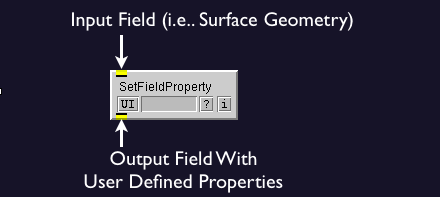
\includegraphics[width=12 cm]{ECGToolkitGuide_figures/SetFieldProps.png}
\caption{Module to set properties such as conductivity and if it is a source or boundary surface for the boundary element method.}
\label{SetFieldProp}
\end{center}
\end{figure}

\begin{figure}[H]
\begin{center}
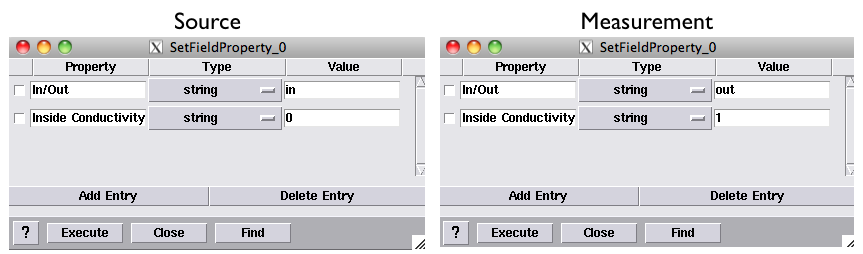
\includegraphics[width=\textwidth]{ECGToolkitGuide_figures/SetFieldPropGUI.png}
\caption{Shows the properties and values needed to create a source surface, left, or a
measurement surface, right.}
\label{SetFieldPropGUI}
\end{center}
\end{figure}


The forward matrix can then be generated by joining all the different surfaces in {\tt BuildBEMatrix} module.
This module will take all the surfaces inputed in the in fields and generate a transfer matrix from the surfaces with the
In/Out field set to the last of the inputed surfaces. Note that the module dynamically adds as many inputs as necessary.

\begin{figure}[H]
\begin{center}
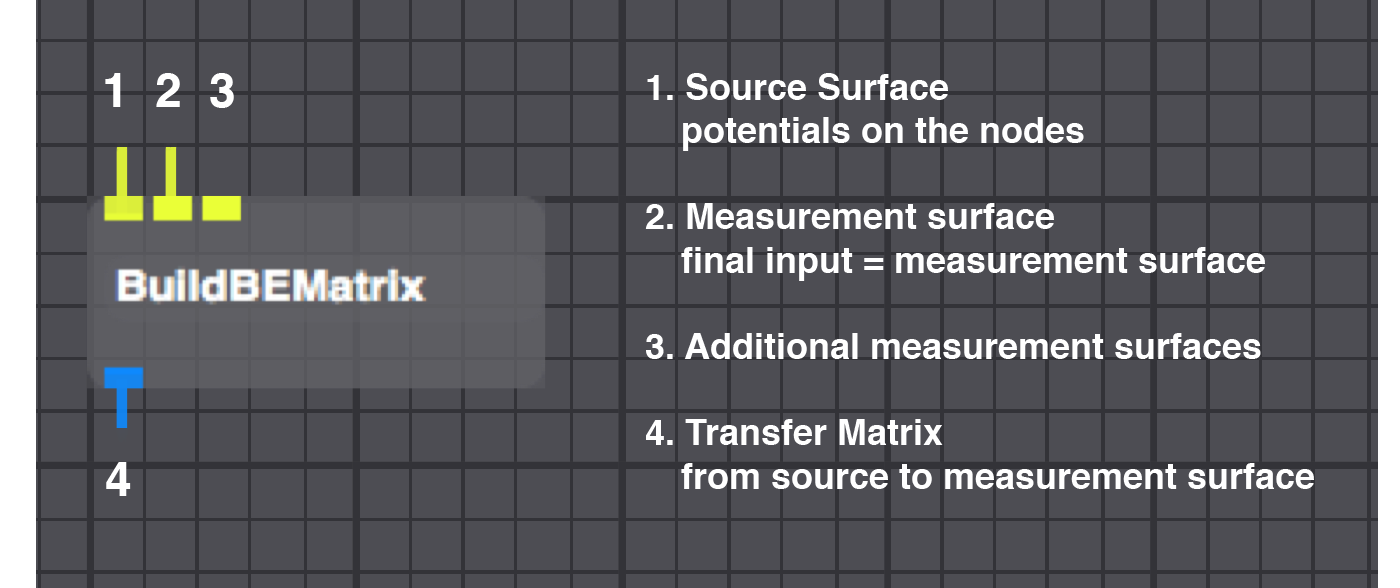
\includegraphics[width=\textwidth]{ECGToolkitGuide_figures/BEMmod.png}
\caption{Shows the module that computes the transfer matrix between the source surface
and the outermost measurement surface.}
\label{BEM}
\end{center}
\end{figure}

{\tt BuildBEMatrix} assumes that, for any closed surface, the surface normals will be pointing outward. The surface
normal for each element is determined using the node order from the connectivity definition of the mesh. The
normals are defined using the right hand rule (counterclockwise) of the node order in each element. The
module {\tt FlipSurfaceNormals} can be used to flip all the element normals in the surface. It is important to check
the normals of the surfaces being used because incorrect normals will produce erroneous answers.

\section{Module Descriptions for Finite Element Solutions}

The two most important modules for the forward finite element solution are the {\tt BuildFEMatrix}
and the {\tt AddKnownsToLinearSystem} modules. These allow you to compute a stiffness matrix and add boundary conditions. The module {\tt BuildFEMatrix} inputs a finite element mesh with the conductivities set on each element, or a lookup table may be used for the conductivities. The result is a stiffness matrix based on the Galerkin method.

\begin{figure}[H]
\begin{center}
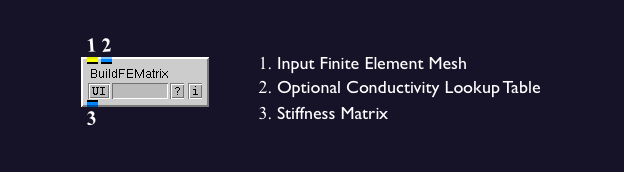
\includegraphics[width=\textwidth]{ECGToolkitGuide_figures/FEMmod.png}
\caption{Shows the module that computes the stiffness matrix for a FE solution.}
\label{FEM}
\end{center}
\end{figure}

{\tt AddKnownsToLinearSystem} makes it possible to add known values as boundary conditions
to the linear system $Ax=b$, where $\mathbf{A}$ is the stiffness matrix, $\mathbf{b}$ is the right hand side vector, and
$\mathbf{x}$ is known in the forward problem and unknown in the inverse problem. The module must have stiffness matrix along with an $\mathbf{x}$ matrix. If no right-hand-side matrix is provided, then it is assumed to be all zeros. Know parameters are input along with the unknown values, while the unknown
values are set to 'nan'.

\begin{figure}[H]
\begin{center}
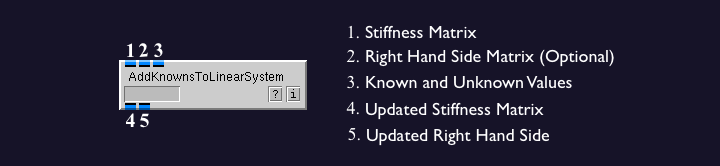
\includegraphics[width=\textwidth]{ECGToolkitGuide_figures/AddKnowns.png}
\caption{Shows the module that computes the stiffness matrix for a FE solution.}
\label{AddKnowns}
\end{center}
\end{figure}


\section{Example Networks for Boundary Element Solutions}

The following network shows the most basic implementation of the boundary element method
along with visualizing the results. This network reads in an epicardial surface mesh that has an associated matrix of epicardial potentials at each node. The conductivities of the torso and heart
are set, along with the differentiation between source and measurement surfaces in the  {\tt SetFieldProperties} module. Next, a boundary element transfer matrix is computed and multiplied with the epicardial potentials. This results in a torso potential field that can be visualized with SCIRun's {\tt ShowField} module.

\begin{figure}[H]
\begin{center}
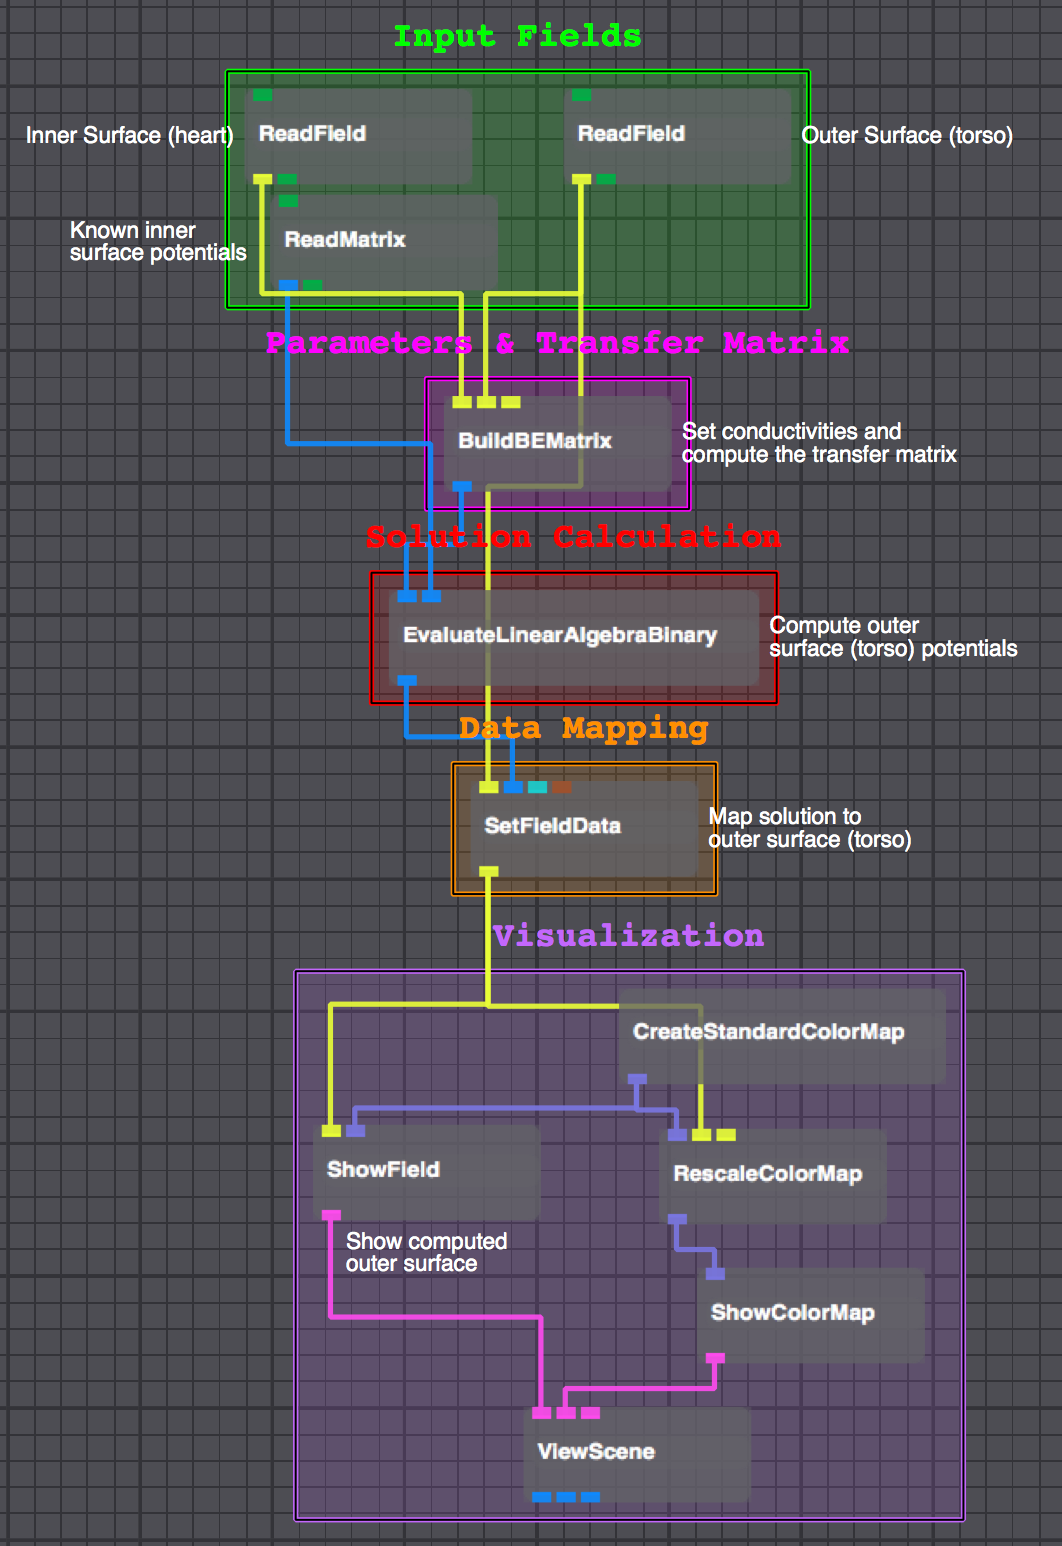
\includegraphics[width=\textwidth]{ECGToolkitGuide_figures/BEMnetwork.png}
\caption{Shows the implementation of the boundary element method.}
\label{BEMnet}
\end{center}
\end{figure}

\vspace{5pt}\textit{A similar SCIRun network for this example can be found at:\\{\tt src/nets/FwdInvToolbox/potential-based-bem/torso-tank-bem.srn}\\in the SCIRun source code directory.}\vspace{5pt}

\section{Example Networks for Finite Element Solutions}

\subsection{Potential Based Forward FEM simulation}

\label{sec:pot_for_fem}
\begin{figure}[H]
\begin{center}
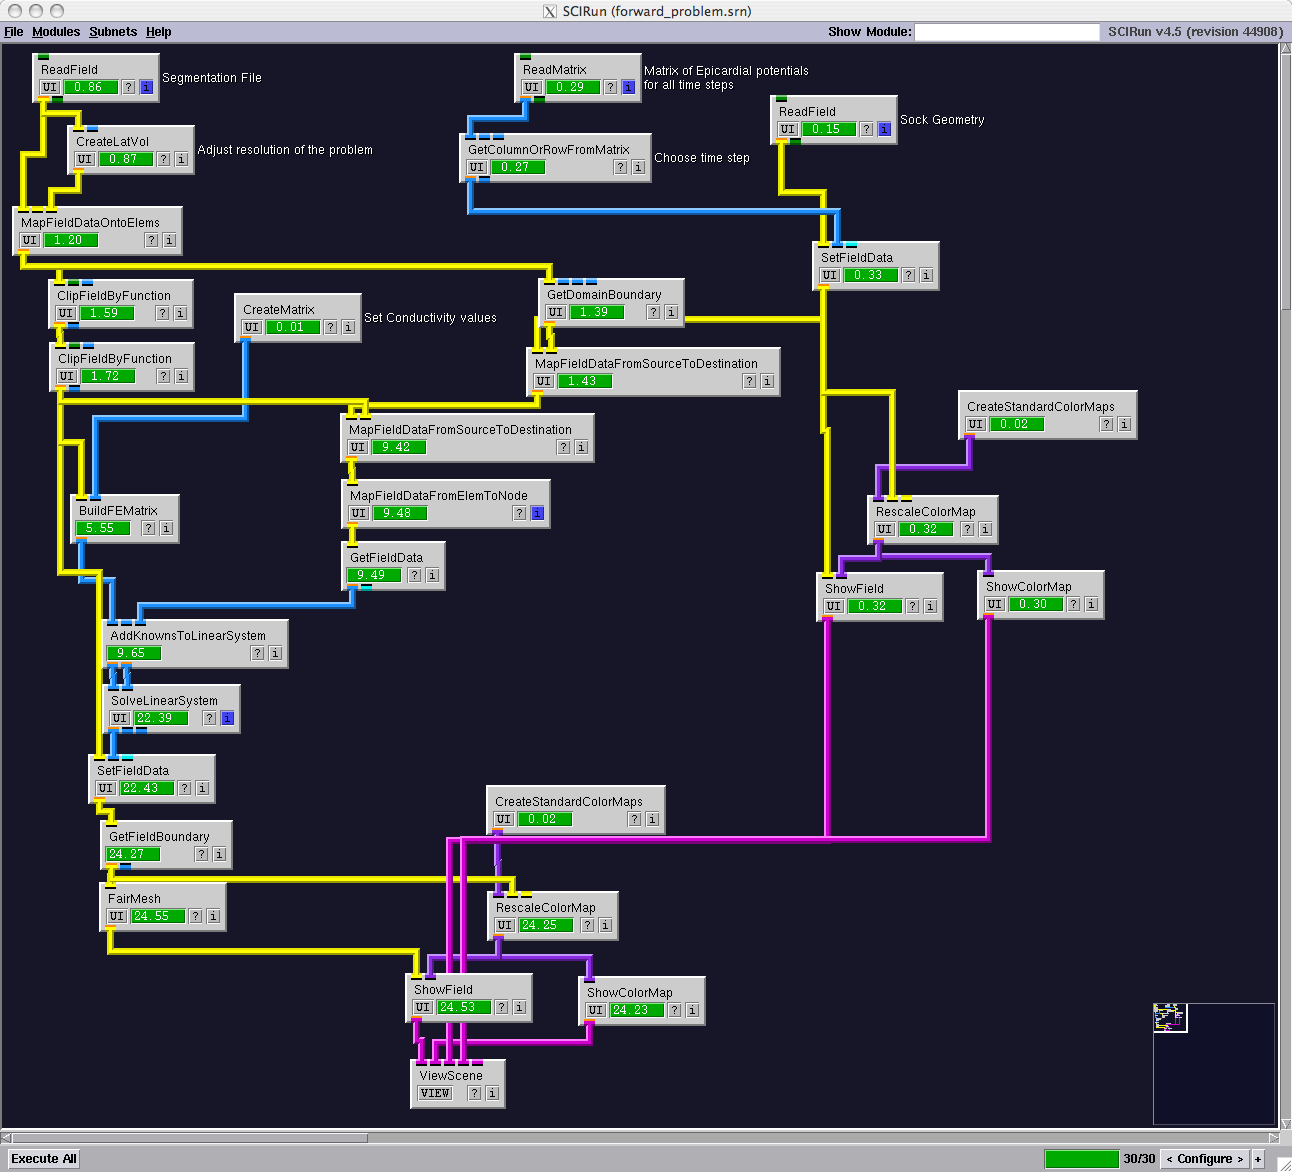
\includegraphics[trim = 5mm 0mm 50mm 0mm, clip, width=\textwidth]{ECGToolkitGuide_figures/potential_forward_fem.png}
\caption{Simple potential based forward problem using FEM.}
\label{fig:pot_for_fem}
\end{center}
\end{figure}

\newpage

There are two examples given to calculate the potential-based forward problem using finite element method. One example involves the generation of the lead field matrix, or transfer matrix, then performing the forward calculation. The other example is a direct calculation of the projection of the cardiac potentials onto the torso surface, satisfying Laplace's equation.


The inputs to the example networks in this section are all the same: a torso segmentation including segmentation of the heart volume with a closed epicardium, a cardiac sock geometry registered to the heart volume from the segmentation, and a matrix of epicardial recordings that were obtained with an epicardial sock. To calculate the lead field matrix, an identity matrix is also used for input vectors.


The example network\\
{\tt src/nets/FwdInvToolbox/potential-based-fem/forward\_problem.srn} provides an example of an easy implementation of the projection of the cardiac potentials onto the torso surface (Figure~\ref{fig:pot_for_fem}). Though this problem is not formulated in the classic sense of the forward problem, it is useful because it does not require calculating the lead field matrix, which can take longer to compute in most cases. The example presented is useful if a forward calculation requires a few time-instances for a given geometry. Different time points may be selected in the {\tt GetColumnOrRowFromMatrix} module.

As mentioned above, the method implemented in this network uses Laplace's equation to find the torso potentials. That is, all the potentials in the torso satisfy the expression:
\begin{equation*}
\nabla \sigma \nabla \phi = 0
\end{equation*}

\noindent where $\phi$ are the potentials and $\sigma$ are the conductivity values. Using SCIRun, one is able to use the cardiac surface potentials as known values and solve the rest of the torso potentials to satisfy Laplace's equation as a linear system.

The example network\\
{\tt potential-based-fem/forward\_problem\_with\_lead\_field\_matrix.srn} is a network that computes the forward problem in a more traditionally understood method (Figure~\ref{fig:pot_for_fem_w_mat}), in that it is a simple matrix multiplication to calculate the torso potentials. This network simply uses a pre-computed lead field matrix and multiplies it by the cardiac potentials to yield the surface torso potentials. Different time points may be selected in the {\tt GetColumnOrRowFromMatrix} module.

\begin{figure}[H]
\begin{center}
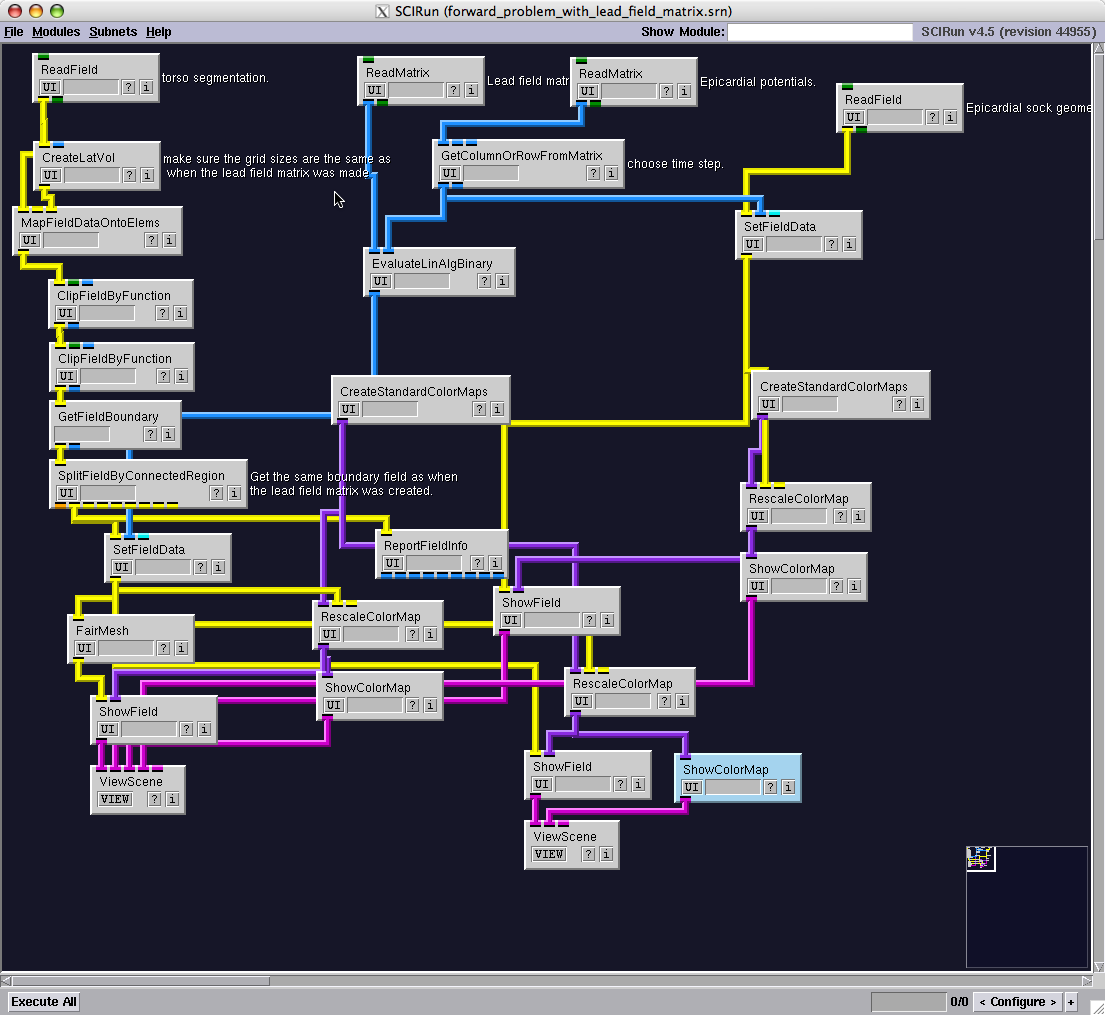
\includegraphics[width=\textwidth]{ECGToolkitGuide_figures/potential_forward_fem_with_leadfield.png}
\caption{Simple potential based forward problem using a pre-computed lead field matrix.}
\label{fig:pot_for_fem_w_mat}
\end{center}
\end{figure}

The lead field matrix provided was generated by the network \newline
{\tt src/nets/FwdInvToolbox/potential-based-fem/Make\_Lead\_field\_matrix.srn} (Figure~\ref{fig:mat_pot_fem}).
This network solves and collects the solution vectors relating isolated points on the heart to the torso. The solution vector is calculated in the same manner as in the network \newline
{\tt src/nets/FwdInvToolbox/potential-based-fem/forward\_problem.srn} described above, using orthogonal unit vectors as the cardiac potential (value of 1 at the point of interest and 0 elsewhere). Computing the lead field matrix this way is very useful if several forward calculations are needed on the same geometry.

\begin{figure}[H]
\begin{center}
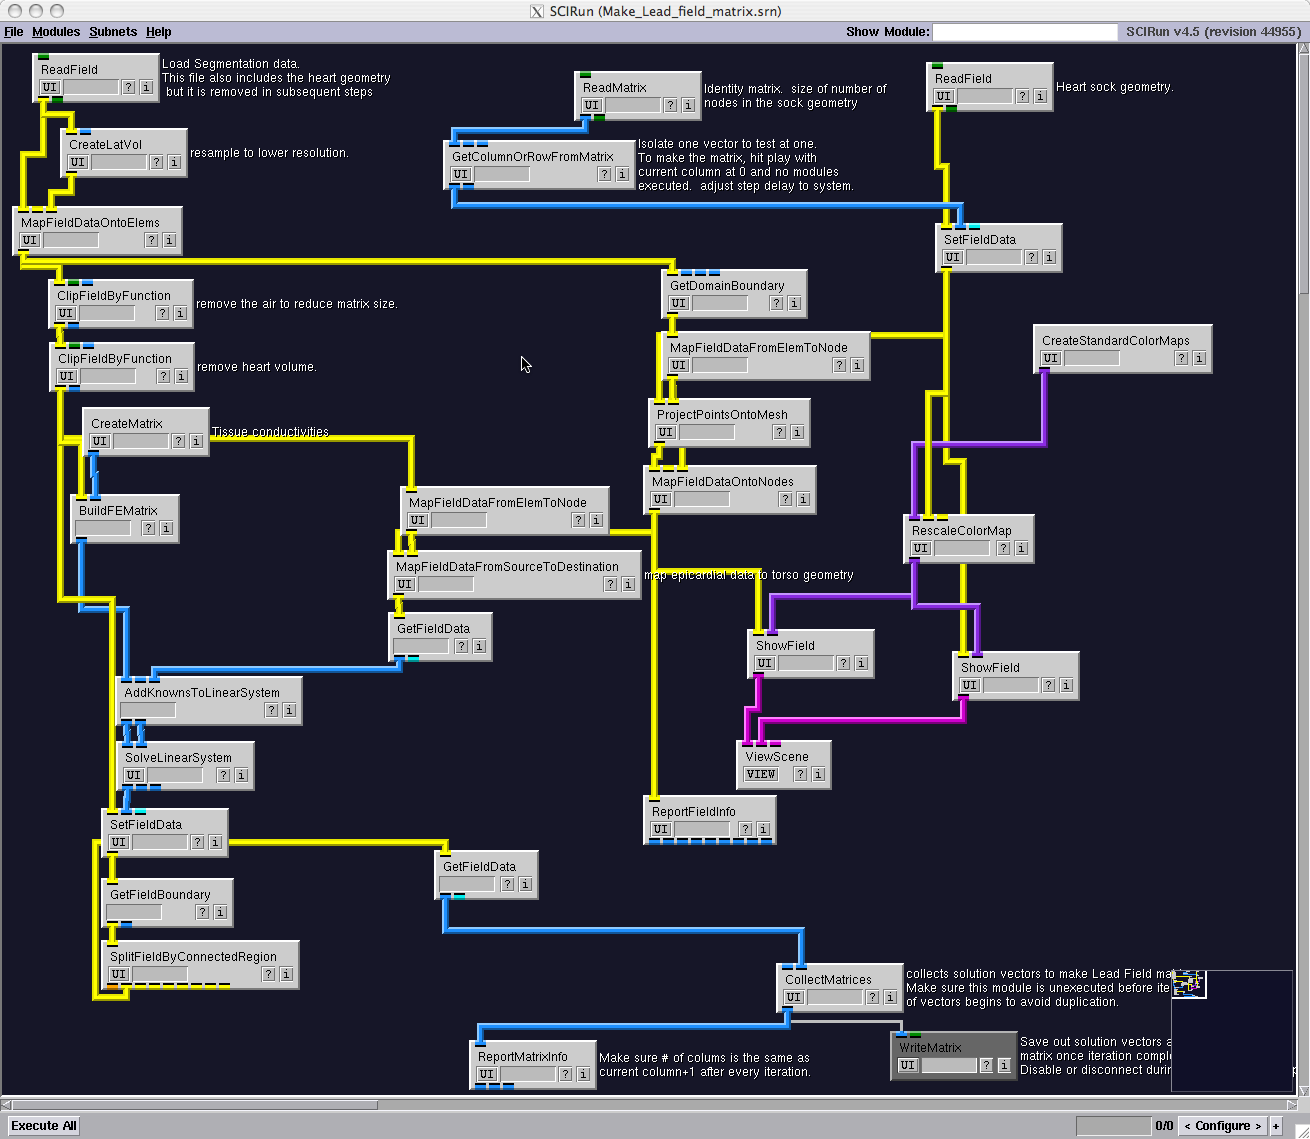
\includegraphics[width=\textwidth]{ECGToolkitGuide_figures/leadfield_pot_fem.png}
\caption{Computing the FEM based lead field matrix.}
\label{fig:mat_pot_fem}
\end{center}
\end{figure}

To calculate the lead field matrix with
\newline \indent{\tt  src/nets/FwdInvToolbox/potential-based-fem/Make\_Lead\_field\_matrix.srn}:
\begin{enumerate}
\item{Make sure the {\tt CollectMatrices} module has not been executed.}
\item{Set step delay in the {\tt GetColumnOrRowFromMatrix} module to a sufficient interval so
that all the modules can fully execute before the next iteration.}
\item{Set the current column to 0 and press ``plays'' in the {\tt GetColumnOrRowFromMatrix}.}
\item{After the network finishes iterating, enable the {\tt WriteMatrix} module (by right clicking on
the module), choose the place and name of the matrix you would like, and press save.  }
\end{enumerate}

\begin{figure}[H]
\begin{center}
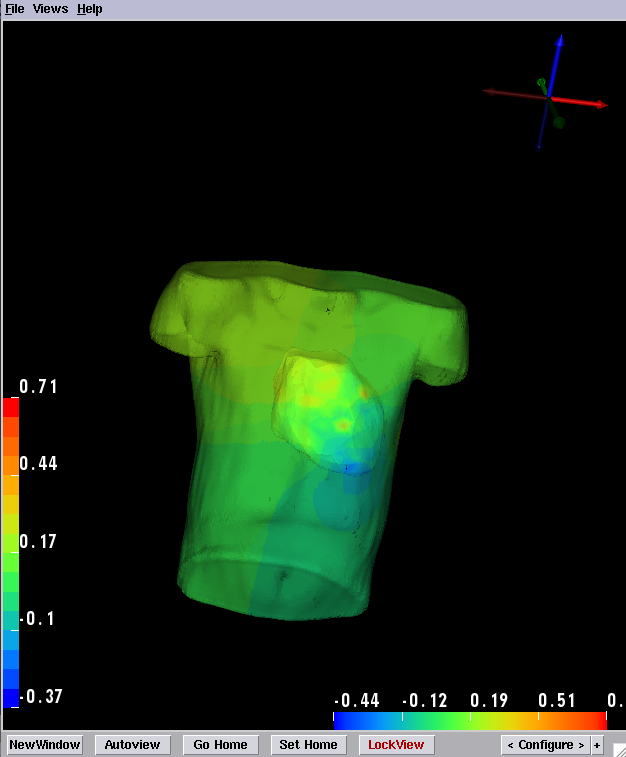
\includegraphics[width=\textwidth]{ECGToolkitGuide_figures/pot_fem_forward_output.png}
\caption{Solution of the potential based forward problem using FEM.}
\label{fig:pot_fem_for_sol}
\end{center}
\end{figure}



\subsection{Activation Based Forward FEM simulation}

The technique used by the activation-based model is rather different than
the potential-based one. These methods, instead of searching solely for the
potentials, consider whether a region of the heart is ``active'' or not and
which is the profile of its potential. This is very different than the activation
profile on a cellular level, as each surface node represents a large region of the
heart. The activation profile is used to specify the strength, in time, of
dipoles located on the surface.

Since FEM is a volume method, SCIRun approximates the volume potentials
by first clipping it with the surface mesh of the inner and outer boundaries.
With this, it obtains a volume mesh that roughly follows the surface. Then, the
potentials of this volume mesh are set so that they approximate the dipoles
on the heart surface. This representation is known as the equivalent dipole
layer.

There are three networks located in {\tt  src/nets/FwdInvToolbox/activation-based-fem}
which provide an example of activation-based forward calculation
using FEM. The three networks are similar in nature to the potential-based
FEM forward problem networks explained in Sec.~\ref{sec:pot_for_fem}.
The activation-based forward problem networks use data derived from ECGSIM.
The surface mesh and source parameters are also obtained from the ECGSIM
project.

The primary inputs to this network are the surface mesh representing
the heart, a torso surface mesh which is made a volume mesh
(refined near the surface of the heart) in the network, and
a matrix specifying the activation profile for each point in the heart
surface mesh at each time to be simulated. This matrix is then of size
$N \times M$ where $N$ is the number of surface points and $M$ is the
number of time-steps represented. A very good example of the input
expected can be obtained from the ECGSIM software by choosing {\em
Save $\rightarrow$ Source parameters} from the {\em File} menu.

Though the {\tt activation-based-fem.srn} networks seem quite complicated,
they perform some simple tasks. The loaded torso surface is made into a
volume and refined in nearer to the heart. Then, two cardiac surfaces are
made from the first, one slightly inside the heart, and one slightly outside.
The corresponding points on the two surfaces are set to either active or inactive.
If the point is inactive, then it is set as an unknown and will be solved for later. If
the point is active, the two surfaces are set to opposing values to approximate a
dipole layer. The remaining torso potentials are solved using a linear-systems
solver similar to Sec.~\ref{sec:pot_for_fem}.

The network {\tt activation-based-fem\_lead\_field.srn} produces similar results
as the previous network, but it utilizes a pre-computed lead field matrix. This
network allows for the activation times to be directly related to the torso surface
and the computation is relatively quick. This method is also more like the
traditionally formulated forward problem with a simple matrix multiply.

The lead field matrix is calculated using the {\tt make\_lead\_field.srn} network.
Similar to the potential-based approach (Sec.~\ref{sec:pot_for_fem}), the solution
vectors for each point on the cardiac surface are calculated and collected as the
lead field matrix. This is essentially a pre-computation of the contribution of each
point. This calculation is very useful if the geometry is going to be used many times.


To calculate the lead field matrix with {\tt make\_lead\_field.srn}:
\begin{enumerate}
\item{Make sure the {\tt CollectMatrices} module has not been executed.}
\item{Set step delay in the {\tt GetColumnOrRowFromMatrix} module is set to a sufficient interval so that all the modules can fully execute before the next iteration.}
\item{Set the current column to 0 and press ``play'' in the {\tt GetColumnOrRowFromMatrix}.}
\item{After the network finishes iterating, enable the {\tt WriteMatrix} module (by right clicking on the module), choose the place and name of the matrix you would like, and press save.  }
\end{enumerate}

\begin{figure}[H]
\begin{center}
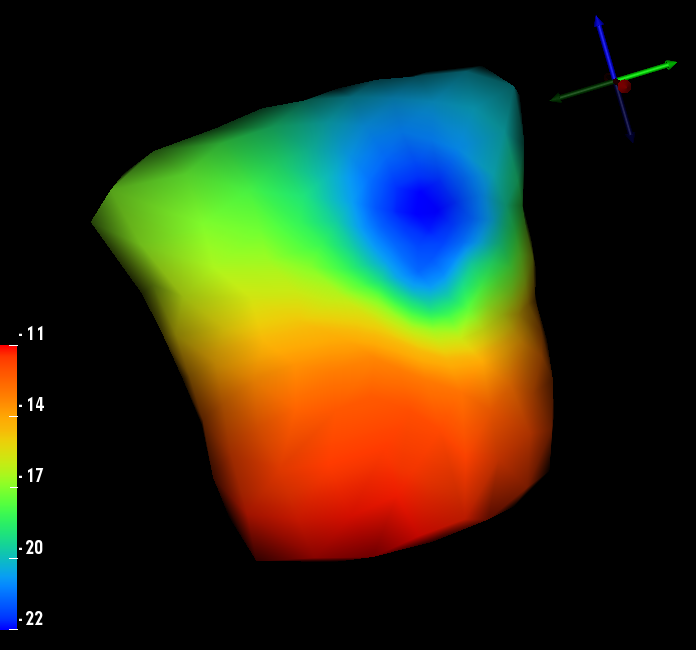
\includegraphics[width=\textwidth]{ECGToolkitGuide_figures/act_for_fem_results.png}
\caption{Solution of the activation based forward problem using FEM.}
\label{fig:act_fem_for_sol}
\end{center}
\end{figure}



\chapter{Forward Solutions}\label{ch:fwd}

\section{Overview}

As described previously, the solution to the forward problem deals with the calculation of the projection of properties from a source, through some medium, to a set of collection locations. In this application, we will demonstrate that the forward problem specifically means the calculation of torso surface potentials from known cardiac source parameters. There are two aspects of the forward problem that one must consider in order to solve it: how to model the source and how that source maps to the torso surface. If presented as the classic $y=A(x)$,  with $y$ as the torso surface and $x$ as the cardiac source, choosing a model that is represented by $x$ is the source formulation. $A$ is then dependent on the source model used, which must represent all relevant information about the torso geometry.

In regard to the source formulation, the two most common models are cardiac potentials and activation times. The use of cardiac potentials is a more intuitive formulation in that the cardiac cells interact to change the extracellular potentials of the myocardium. These potentials then project to the torso surface. The activation-time-based source formulation deals with the fact that when there is inactive and active tissue next to each other, a source much like a dipole or layer of dipoles is generated, which then projects to the surface. Both of these source models contain several assumptions, but each provides a generally accurate model that can be computationally reasonable.

With the source formulation considered, one must now determine the pattern with which the source projects to the torso surface. As mentioned, this relationship is dependent on the source model as well as the various properties of the torso. But in both source models presented, the function $A$ can be represented by an $N \times M$ matrix. $N$ is the number of points on the cardiac surface and $M$ the number of points on the torso surface, which is called the lead field matrix. Calculating this matrix can be a very computationally intensive task, and there are varying ways to do this. The two examples given here find the lead field, or transfer matrix, are based on finite element method (FEM) and boundary element method (BEM). The theory and mathematics behind these two methods are presented in Ch. ~\ref{sec:ch1}.

We provide in this toolkit three methods to calculate the forward problem. Potential based models using both FEM and BEM are demonstrated, as well as an activation-time based model using FEM. The BEM activation-time forward problem is not yet supported in SCIRun, but it is performed in ECGSim, the interactive simulation software developed by Peacs in the Netherlands.\footnote{To obtain this free software, visit http://www.ecgsim.org/. Any references to ECGSIM herein are referring to version 1.3 beta}.


An equivalent dipole layer is approximated as the source in the activation based forward problem.


\section{Module Descriptions for Boundary Element Solutions}

The boundary element solution utilizes many common modules within the SCIRun framework
to read in files, visualize data, and manipulate geometry. Descriptions of these modules
can be found in the SCIRun documentation, whereas the modules that are relatively unique to the boundary element solution are outlined below.

The first module to be introduced is {\tt SetFieldProperties}. This module is thought to generate and modify properties of an input field, such as the potentials and conductivities of
the epicardial surface. Figure \ref{SetFieldPropGUI} shows an example of how epicardial and torso surfaces should be defined. Since the heart surface is associated with epicardial potentials,
it must have conductivity set to 0. On the other hand, the torso and the lungs are measurement surfaces and should have their respective conductivity value.\\
With the {\tt SetFieldProperties} GUI, the user can define a set of desired properties of the input field and the corresponding values.

\begin{figure}[H]
\begin{center}
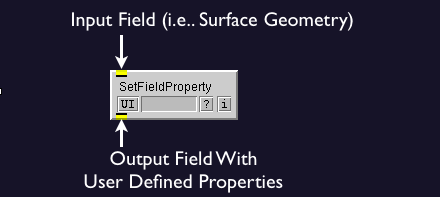
\includegraphics[width=12 cm]{ECGToolkitGuide_figures/SetFieldProps.png}
\caption{Module to set properties such as conductivity and if it is a source or boundary surface for the boundary element method.}
\label{SetFieldProp}
\end{center}
\end{figure}

\begin{figure}[H]
\begin{center}
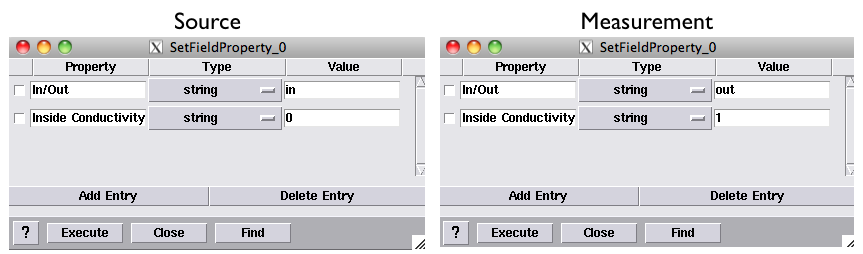
\includegraphics[width=\textwidth]{ECGToolkitGuide_figures/SetFieldPropGUI.png}
\caption{Shows the properties and values needed to create a source surface, left, or a
measurement surface, right.}
\label{SetFieldPropGUI}
\end{center}
\end{figure}


The forward matrix can then be generated by joining all the different surfaces in {\tt BuildBEMatrix} module.
This module will take all the surfaces inputed in the in fields and generate a transfer matrix from the surfaces with the
In/Out field set to the last of the inputed surfaces. Note that the module dynamically adds as many inputs as necessary.

\begin{figure}[H]
\begin{center}
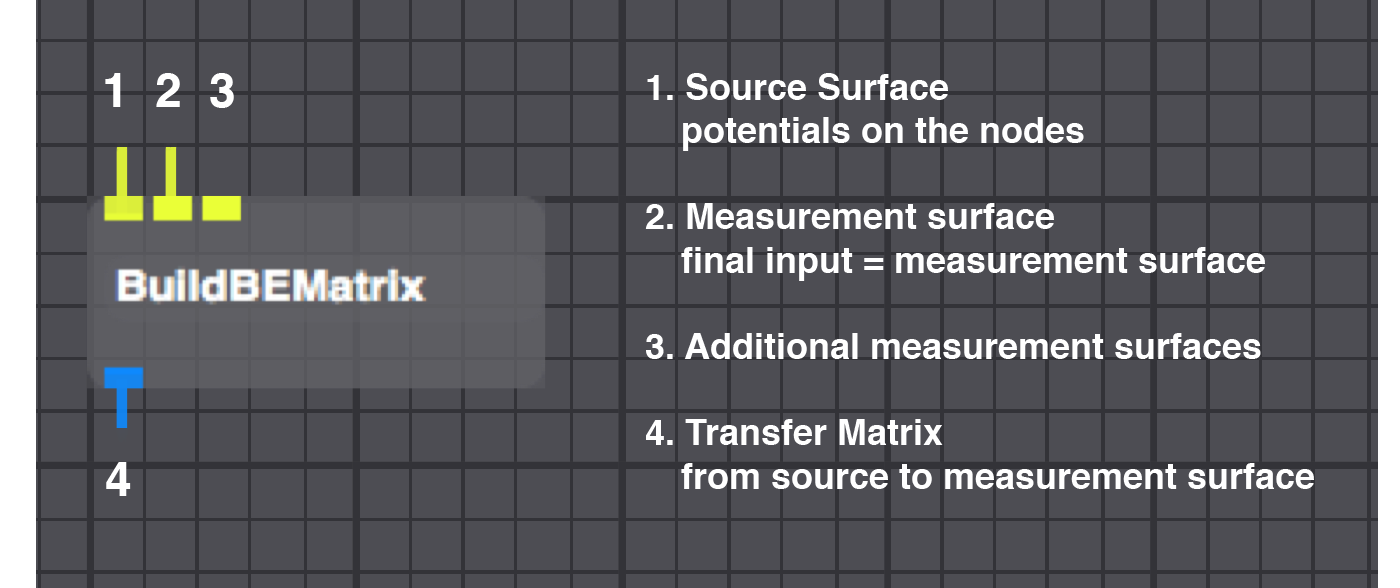
\includegraphics[width=\textwidth]{ECGToolkitGuide_figures/BEMmod.png}
\caption{Shows the module that computes the transfer matrix between the source surface
and the outermost measurement surface.}
\label{BEM}
\end{center}
\end{figure}

{\tt BuildBEMatrix} assumes that, for any closed surface, the surface normals will be pointing outward. The surface
normal for each element is determined using the node order from the connectivity definition of the mesh. The
normals are defined using the right hand rule (counterclockwise) of the node order in each element. The
module {\tt FlipSurfaceNormals} can be used to flip all the element normals in the surface. It is important to check
the normals of the surfaces being used because incorrect normals will produce erroneous answers.

\section{Module Descriptions for Finite Element Solutions}

The two most important modules for the forward finite element solution are the {\tt BuildFEMatrix}
and the {\tt AddKnownsToLinearSystem} modules. These allow you to compute a stiffness matrix and add boundary conditions. The module {\tt BuildFEMatrix} inputs a finite element mesh with the conductivities set on each element, or a lookup table may be used for the conductivities. The result is a stiffness matrix based on the Galerkin method.

\begin{figure}[H]
\begin{center}
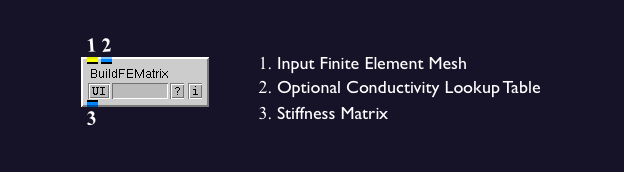
\includegraphics[width=\textwidth]{ECGToolkitGuide_figures/FEMmod.png}
\caption{Shows the module that computes the stiffness matrix for a FE solution.}
\label{FEM}
\end{center}
\end{figure}

{\tt AddKnownsToLinearSystem} makes it possible to add known values as boundary conditions
to the linear system $Ax=b$, where $\mathbf{A}$ is the stiffness matrix, $\mathbf{b}$ is the right hand side vector, and
$\mathbf{x}$ is known in the forward problem and unknown in the inverse problem. The module must have stiffness matrix along with an $\mathbf{x}$ matrix. If no right-hand-side matrix is provided, then it is assumed to be all zeros. Know parameters are input along with the unknown values, while the unknown
values are set to 'nan'.

\begin{figure}[H]
\begin{center}
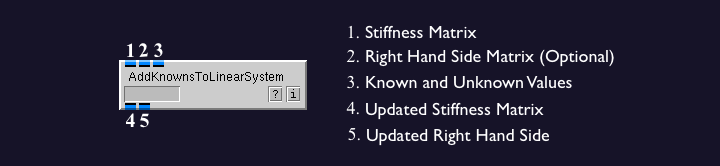
\includegraphics[width=\textwidth]{ECGToolkitGuide_figures/AddKnowns.png}
\caption{Shows the module that computes the stiffness matrix for a FE solution.}
\label{AddKnowns}
\end{center}
\end{figure}


\section{Example Networks for Boundary Element Solutions}

The following network shows the most basic implementation of the boundary element method
along with visualizing the results. This network reads in an epicardial surface mesh that has an associated matrix of epicardial potentials at each node. The conductivities of the torso and heart
are set, along with the differentiation between source and measurement surfaces in the  {\tt SetFieldProperties} module. Next, a boundary element transfer matrix is computed and multiplied with the epicardial potentials. This results in a torso potential field that can be visualized with SCIRun's {\tt ShowField} module.

\begin{figure}[H]
\begin{center}
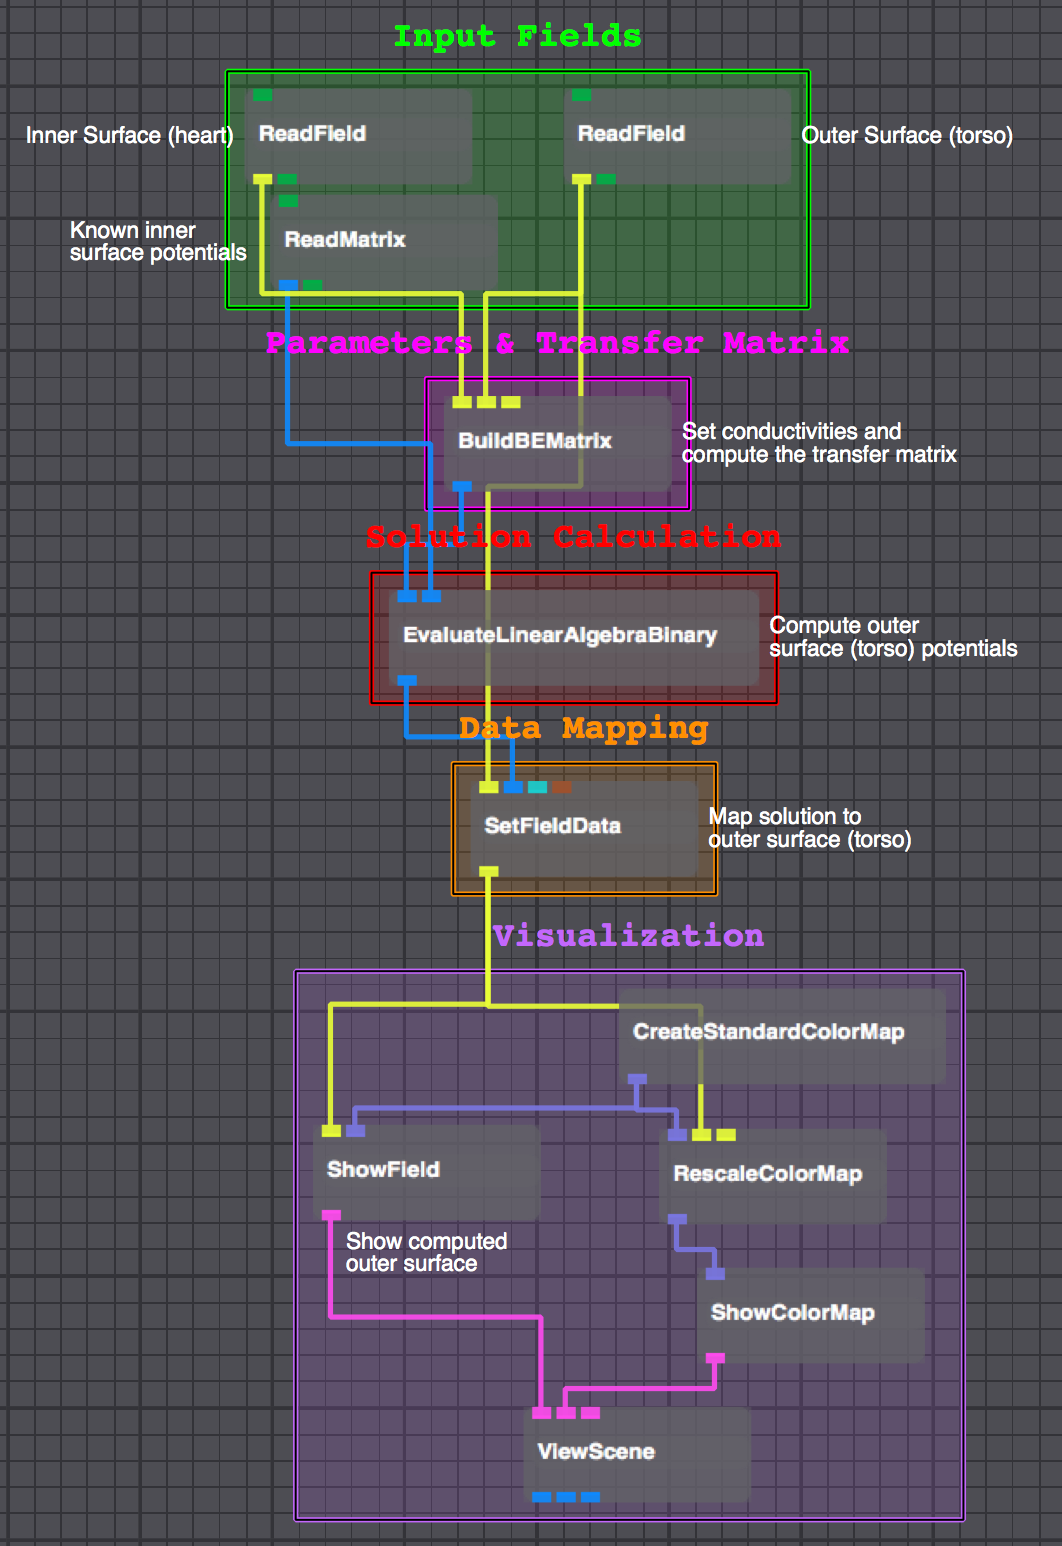
\includegraphics[width=\textwidth]{ECGToolkitGuide_figures/BEMnetwork.png}
\caption{Shows the implementation of the boundary element method.}
\label{BEMnet}
\end{center}
\end{figure}

\vspace{5pt}\textit{A similar SCIRun network for this example can be found at:\\{\tt src/nets/FwdInvToolbox/potential-based-bem/torso-tank-bem.srn}\\in the SCIRun source code directory.}\vspace{5pt}

\section{Example Networks for Finite Element Solutions}

\subsection{Potential Based Forward FEM simulation}

\label{sec:pot_for_fem}
\begin{figure}[H]
\begin{center}
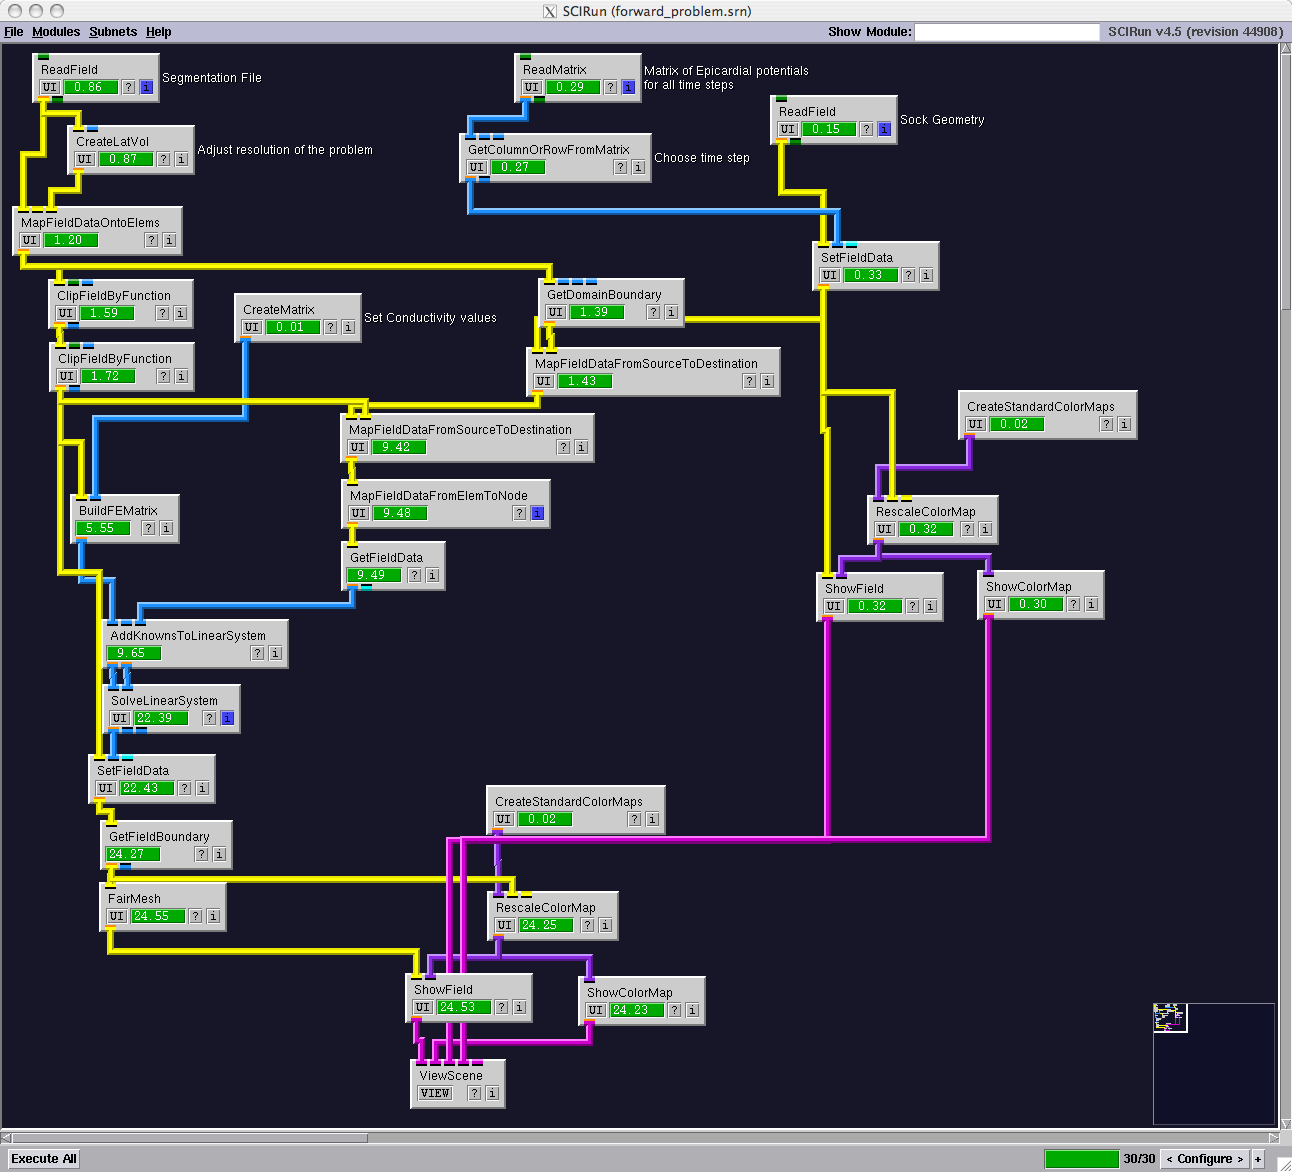
\includegraphics[trim = 5mm 0mm 50mm 0mm, clip, width=\textwidth]{ECGToolkitGuide_figures/potential_forward_fem.png}
\caption{Simple potential based forward problem using FEM.}
\label{fig:pot_for_fem}
\end{center}
\end{figure}

\newpage

There are two examples given to calculate the potential-based forward problem using finite element method. One example involves the generation of the lead field matrix, or transfer matrix, then performing the forward calculation. The other example is a direct calculation of the projection of the cardiac potentials onto the torso surface, satisfying Laplace's equation.


The inputs to the example networks in this section are all the same: a torso segmentation including segmentation of the heart volume with a closed epicardium, a cardiac sock geometry registered to the heart volume from the segmentation, and a matrix of epicardial recordings that were obtained with an epicardial sock. To calculate the lead field matrix, an identity matrix is also used for input vectors.


The example network\\
{\tt src/nets/FwdInvToolbox/potential-based-fem/forward\_problem.srn} provides an example of an easy implementation of the projection of the cardiac potentials onto the torso surface (Figure~\ref{fig:pot_for_fem}). Though this problem is not formulated in the classic sense of the forward problem, it is useful because it does not require calculating the lead field matrix, which can take longer to compute in most cases. The example presented is useful if a forward calculation requires a few time-instances for a given geometry. Different time points may be selected in the {\tt GetColumnOrRowFromMatrix} module.

As mentioned above, the method implemented in this network uses Laplace's equation to find the torso potentials. That is, all the potentials in the torso satisfy the expression:
\begin{equation*}
\nabla \sigma \nabla \phi = 0
\end{equation*}

\noindent where $\phi$ are the potentials and $\sigma$ are the conductivity values. Using SCIRun, one is able to use the cardiac surface potentials as known values and solve the rest of the torso potentials to satisfy Laplace's equation as a linear system.

The example network\\
{\tt potential-based-fem/forward\_problem\_with\_lead\_field\_matrix.srn} is a network that computes the forward problem in a more traditionally understood method (Figure~\ref{fig:pot_for_fem_w_mat}), in that it is a simple matrix multiplication to calculate the torso potentials. This network simply uses a pre-computed lead field matrix and multiplies it by the cardiac potentials to yield the surface torso potentials. Different time points may be selected in the {\tt GetColumnOrRowFromMatrix} module.

\begin{figure}[H]
\begin{center}
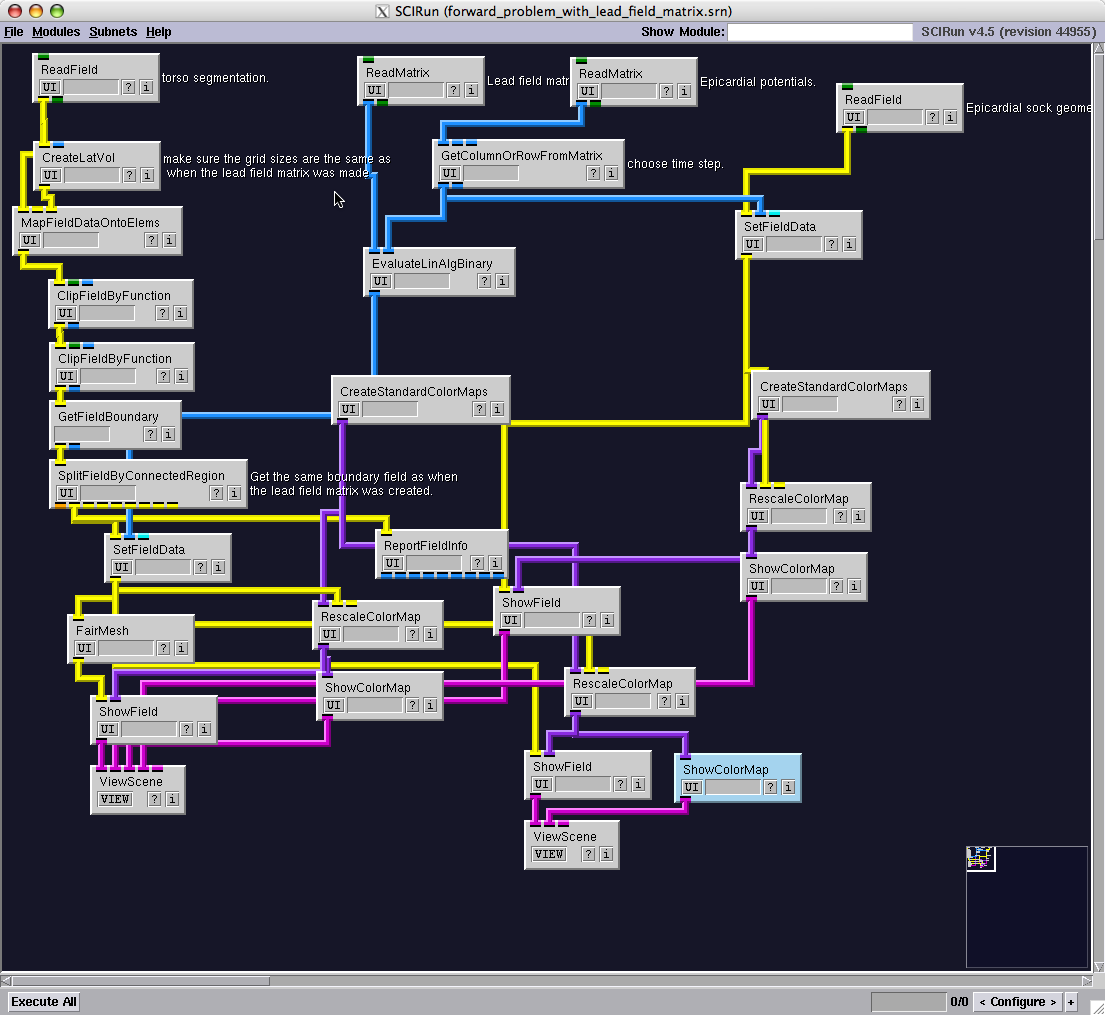
\includegraphics[width=\textwidth]{ECGToolkitGuide_figures/potential_forward_fem_with_leadfield.png}
\caption{Simple potential based forward problem using a pre-computed lead field matrix.}
\label{fig:pot_for_fem_w_mat}
\end{center}
\end{figure}

The lead field matrix provided was generated by the network \newline
{\tt src/nets/FwdInvToolbox/potential-based-fem/Make\_Lead\_field\_matrix.srn} (Figure~\ref{fig:mat_pot_fem}).
This network solves and collects the solution vectors relating isolated points on the heart to the torso. The solution vector is calculated in the same manner as in the network \newline
{\tt src/nets/FwdInvToolbox/potential-based-fem/forward\_problem.srn} described above, using orthogonal unit vectors as the cardiac potential (value of 1 at the point of interest and 0 elsewhere). Computing the lead field matrix this way is very useful if several forward calculations are needed on the same geometry.

\begin{figure}[H]
\begin{center}
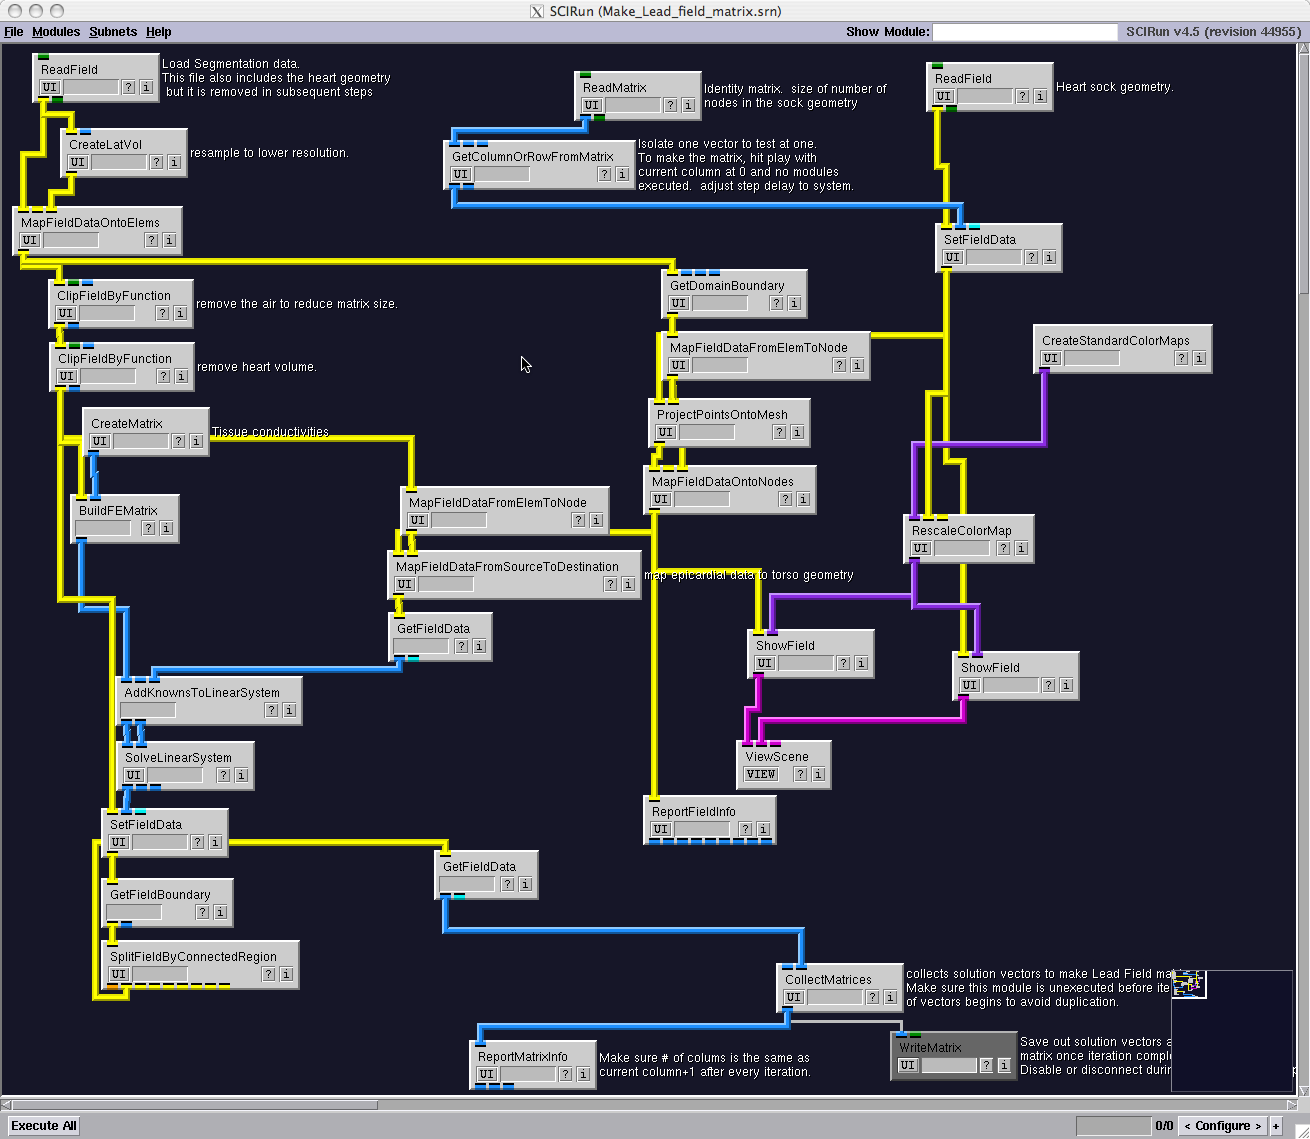
\includegraphics[width=\textwidth]{ECGToolkitGuide_figures/leadfield_pot_fem.png}
\caption{Computing the FEM based lead field matrix.}
\label{fig:mat_pot_fem}
\end{center}
\end{figure}

To calculate the lead field matrix with
\newline \indent{\tt  src/nets/FwdInvToolbox/potential-based-fem/Make\_Lead\_field\_matrix.srn}:
\begin{enumerate}
\item{Make sure the {\tt CollectMatrices} module has not been executed.}
\item{Set step delay in the {\tt GetColumnOrRowFromMatrix} module to a sufficient interval so
that all the modules can fully execute before the next iteration.}
\item{Set the current column to 0 and press ``plays'' in the {\tt GetColumnOrRowFromMatrix}.}
\item{After the network finishes iterating, enable the {\tt WriteMatrix} module (by right clicking on
the module), choose the place and name of the matrix you would like, and press save.  }
\end{enumerate}

\begin{figure}[H]
\begin{center}
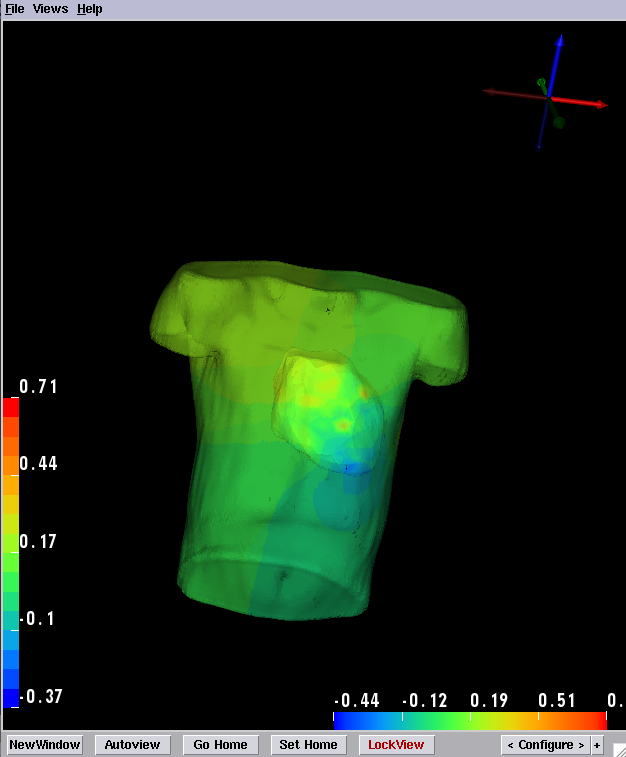
\includegraphics[width=\textwidth]{ECGToolkitGuide_figures/pot_fem_forward_output.png}
\caption{Solution of the potential based forward problem using FEM.}
\label{fig:pot_fem_for_sol}
\end{center}
\end{figure}



\subsection{Activation Based Forward FEM simulation}

The technique used by the activation-based model is rather different than
the potential-based one. These methods, instead of searching solely for the
potentials, consider whether a region of the heart is ``active'' or not and
which is the profile of its potential. This is very different than the activation
profile on a cellular level, as each surface node represents a large region of the
heart. The activation profile is used to specify the strength, in time, of
dipoles located on the surface.

Since FEM is a volume method, SCIRun approximates the volume potentials
by first clipping it with the surface mesh of the inner and outer boundaries.
With this, it obtains a volume mesh that roughly follows the surface. Then, the
potentials of this volume mesh are set so that they approximate the dipoles
on the heart surface. This representation is known as the equivalent dipole
layer.

There are three networks located in {\tt  src/nets/FwdInvToolbox/activation-based-fem}
which provide an example of activation-based forward calculation
using FEM. The three networks are similar in nature to the potential-based
FEM forward problem networks explained in Sec.~\ref{sec:pot_for_fem}.
The activation-based forward problem networks use data derived from ECGSIM.
The surface mesh and source parameters are also obtained from the ECGSIM
project.

The primary inputs to this network are the surface mesh representing
the heart, a torso surface mesh which is made a volume mesh
(refined near the surface of the heart) in the network, and
a matrix specifying the activation profile for each point in the heart
surface mesh at each time to be simulated. This matrix is then of size
$N \times M$ where $N$ is the number of surface points and $M$ is the
number of time-steps represented. A very good example of the input
expected can be obtained from the ECGSIM software by choosing {\em
Save $\rightarrow$ Source parameters} from the {\em File} menu.

Though the {\tt activation-based-fem.srn} networks seem quite complicated,
they perform some simple tasks. The loaded torso surface is made into a
volume and refined in nearer to the heart. Then, two cardiac surfaces are
made from the first, one slightly inside the heart, and one slightly outside.
The corresponding points on the two surfaces are set to either active or inactive.
If the point is inactive, then it is set as an unknown and will be solved for later. If
the point is active, the two surfaces are set to opposing values to approximate a
dipole layer. The remaining torso potentials are solved using a linear-systems
solver similar to Sec.~\ref{sec:pot_for_fem}.

The network {\tt activation-based-fem\_lead\_field.srn} produces similar results
as the previous network, but it utilizes a pre-computed lead field matrix. This
network allows for the activation times to be directly related to the torso surface
and the computation is relatively quick. This method is also more like the
traditionally formulated forward problem with a simple matrix multiply.

The lead field matrix is calculated using the {\tt make\_lead\_field.srn} network.
Similar to the potential-based approach (Sec.~\ref{sec:pot_for_fem}), the solution
vectors for each point on the cardiac surface are calculated and collected as the
lead field matrix. This is essentially a pre-computation of the contribution of each
point. This calculation is very useful if the geometry is going to be used many times.


To calculate the lead field matrix with {\tt make\_lead\_field.srn}:
\begin{enumerate}
\item{Make sure the {\tt CollectMatrices} module has not been executed.}
\item{Set step delay in the {\tt GetColumnOrRowFromMatrix} module is set to a sufficient interval so that all the modules can fully execute before the next iteration.}
\item{Set the current column to 0 and press ``play'' in the {\tt GetColumnOrRowFromMatrix}.}
\item{After the network finishes iterating, enable the {\tt WriteMatrix} module (by right clicking on the module), choose the place and name of the matrix you would like, and press save.  }
\end{enumerate}

\begin{figure}[H]
\begin{center}
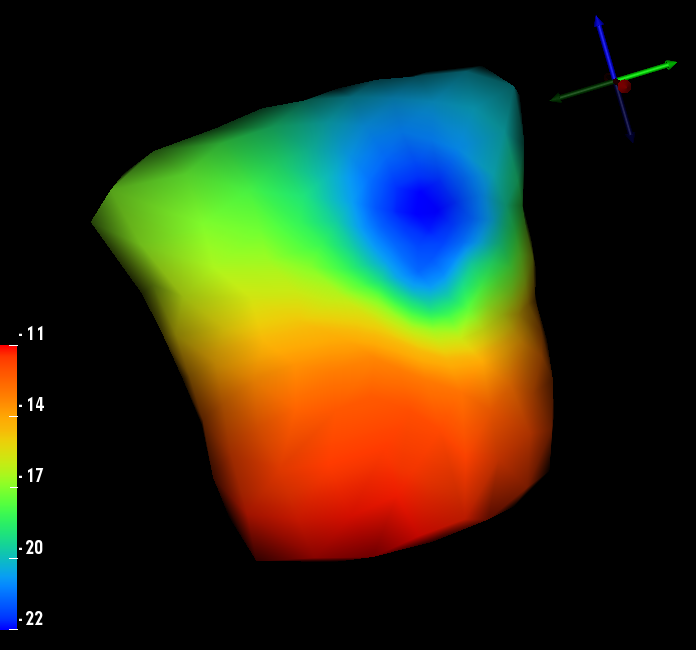
\includegraphics[width=\textwidth]{ECGToolkitGuide_figures/act_for_fem_results.png}
\caption{Solution of the activation based forward problem using FEM.}
\label{fig:act_fem_for_sol}
\end{center}
\end{figure}


% Inverse ---------------------------------------------------------------
%\chapter{Inverse Solutions}
\label{ch:inv}

\section{Overview}

The inverse problem of electrocardiography is to find suitable electrical source parameters on the heart that adequately describe the observed body surface potentials. Regularization is typically employed in solution methods to reduce the sensitivity of the problem to relatively small errors in the observed body surface potentials, thereby stabilizing it. As a result, solution methods may be supplied body surface potentials, a forward model, and method-specific regularization parameters as input. Specific use of each method is described below. As output, modules primarily produce the resulting solution with extra outputs, depending on the specific method.

\section{Descriptions of the Inverse Solution Methods Implemented in SCIRun}

%%%%%%%%%%%%%%%%%%%%%%%
\subsection{Tikhonov Regularization}\label{sec:inverse:tikhonov}

    As described in Sec.~\ref{sec:math_tikhonov}, Tikhonov regularization is a classical inverse method that solves the following least squares problem:
    \begin{center}
        \begin{eqnarray}
            min_{X} \| P (Y - A X) \|^{2}_{2} + \lambda^{2} \| RX \|^{2}_{2},
        \label{eq:inverseSec_tik_problem}
        \end{eqnarray}
    \end{center}
    where $Y$ are the measured ECG potentials, $A$ is the forward matrix, $X$ are the unknown potentials on the heart, $\lambda$ is the regularization parameter, $R$ is a regularization matrix and $P$ is the sensor covariance matrix.
    All these variables can be found as inputs or outputs of the module \href{http://scirundocwiki.sci.utah.edu/SCIRunDocs/index.php/CIBC:Documentation:SCIRun:Reference:BioPSE:SolveInverseProblemWithTikhonov}{{\tt SolveInverseProblemWithTikhonov}}, shown in \autoref{fig:tik_module}.
    \begin{figure}
        \begin{center}
        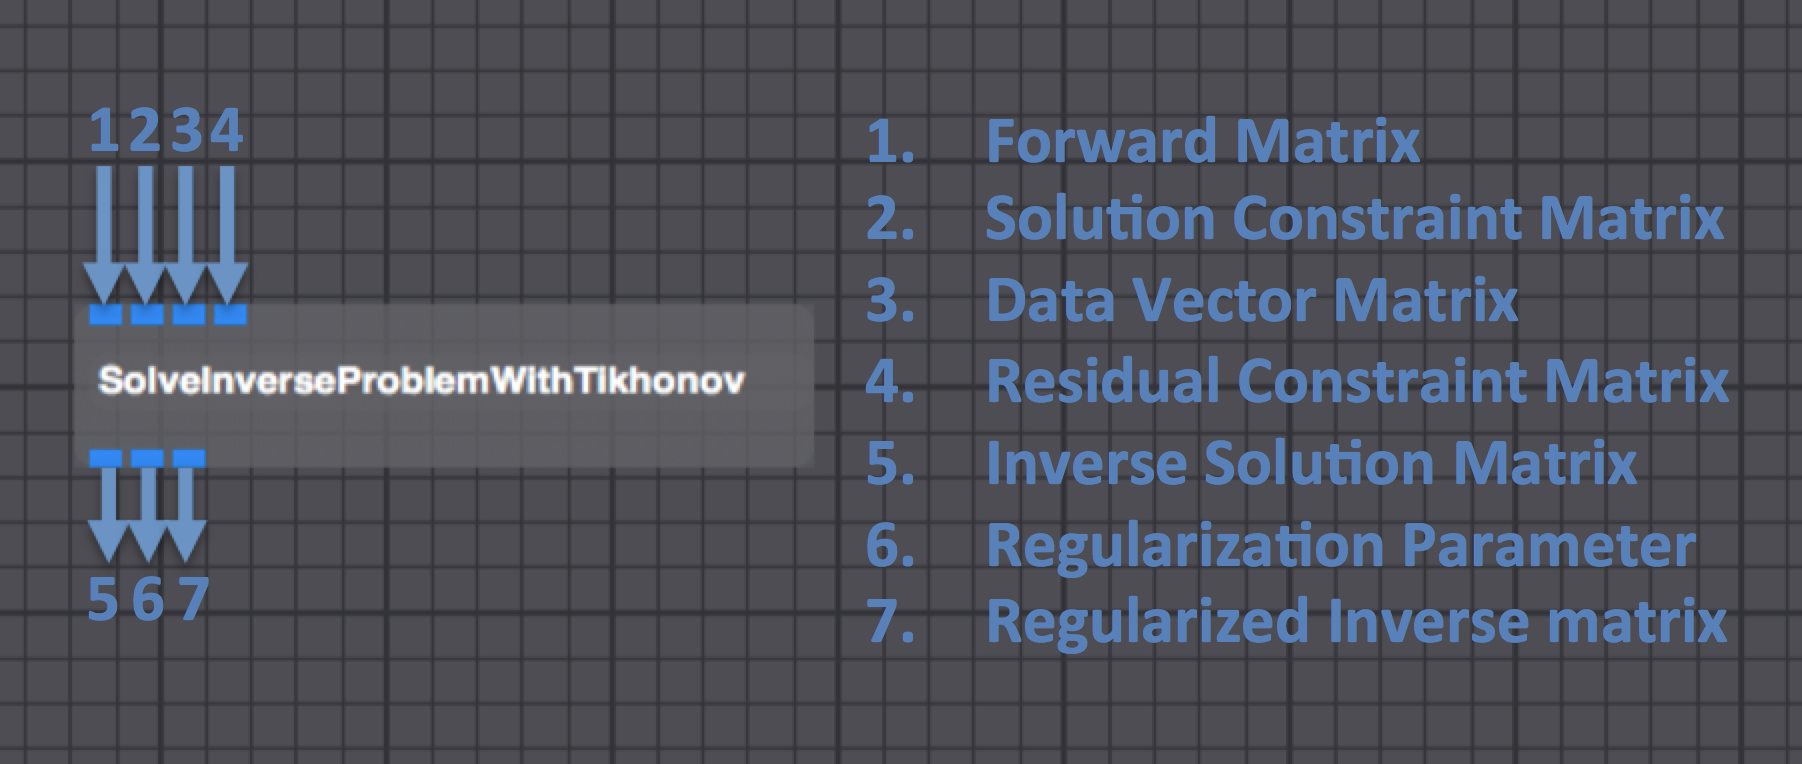
\includegraphics[width=0.7\textwidth]{ECGToolkitGuide_figures/tik1.png}
        \caption{Revised Tikhonov module: {\tt SolveInverseProblemWithTikhonov}.  }
        \label{fig:tik_module}
        \end{center}
    \end{figure}
    \noindent{\bf Inputs:}
    \begin{enumerate}
        \item Forward Matrix ($A\in\Re^{N,M}$)
        \item Weights in Source Space ($R\in\Re^{L,M}$ or squared $R^2\in\Re^{M,M}$ o)
        \item Measured Potentials ($Y\in\Re^{N,T}$)
        \item Weights in Sensor Space ($P\in\Re^{F,N}$ or squared $P^2\in\Re^{N,N}$),
    \end{enumerate}
    {\bf Outputs:}
     \begin{enumerate}
        \item Inverse Solution ($X\in\Re^{M,T}$)
        \item Regularization Parameter ($\lambda$)
        \item Regularized Inverse ($G\in\Re^{M,N}$)
    \end{enumerate}

    An example of the usage of the module \href{http://scirundocwiki.sci.utah.edu/SCIRunDocs/index.php/CIBC:Documentation:SCIRun:Reference:BioPSE:SolveInverseProblemWithTikhonov}{{\tt SolveInverseProblemWithTikhonov}} can be found in the network ``potential-based-inverse/tikhonov-inverse.srn5'', which is shown in \autoref{TikhonovNetworkExample}.
    This example network is composed of four main blocks:
    \begin{itemize}
        \item {\bf Loading Data (green):} These are the modules that load the data into SCIRun.
        \item {\bf Forward Solution (white):} These modules compute simulations of ECG potentials that would be measured on the body surface.
        \item {\bf Tikhonov Inverse (black):} This module computes the Tikhonov inverse solution.
        \item {\bf Visualization (purple):} These modules provide visualization of the solution and the ground truth.
    \end{itemize}

    \subsubsection{Options and Modes of Operation}

    The \href{http://scirundocwiki.sci.utah.edu/SCIRunDocs/index.php/CIBC:Documentation:SCIRun:Reference:BioPSE:SolveInverseProblemWithTikhonov}{{\tt SolveInverseProblemWithTikhonov}} module allows for multiple modes of operation that provide different functionalities and computational advantages.
    These modes of operation, can be found in the two panels of the module user interface, shown in \autoref{fig:tik_module_gui}.
    The options within each of the two panels are described in the following:

    \begin{figure}
    \begin{center}
    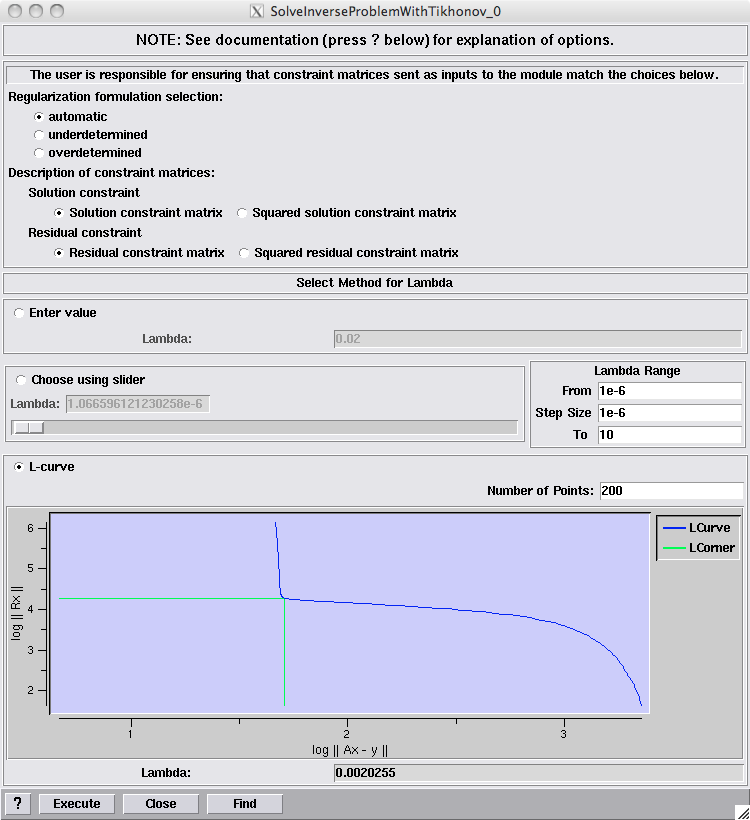
\includegraphics[width=0.45\textwidth]{ECGToolkitGuide_figures/tik2.png}
    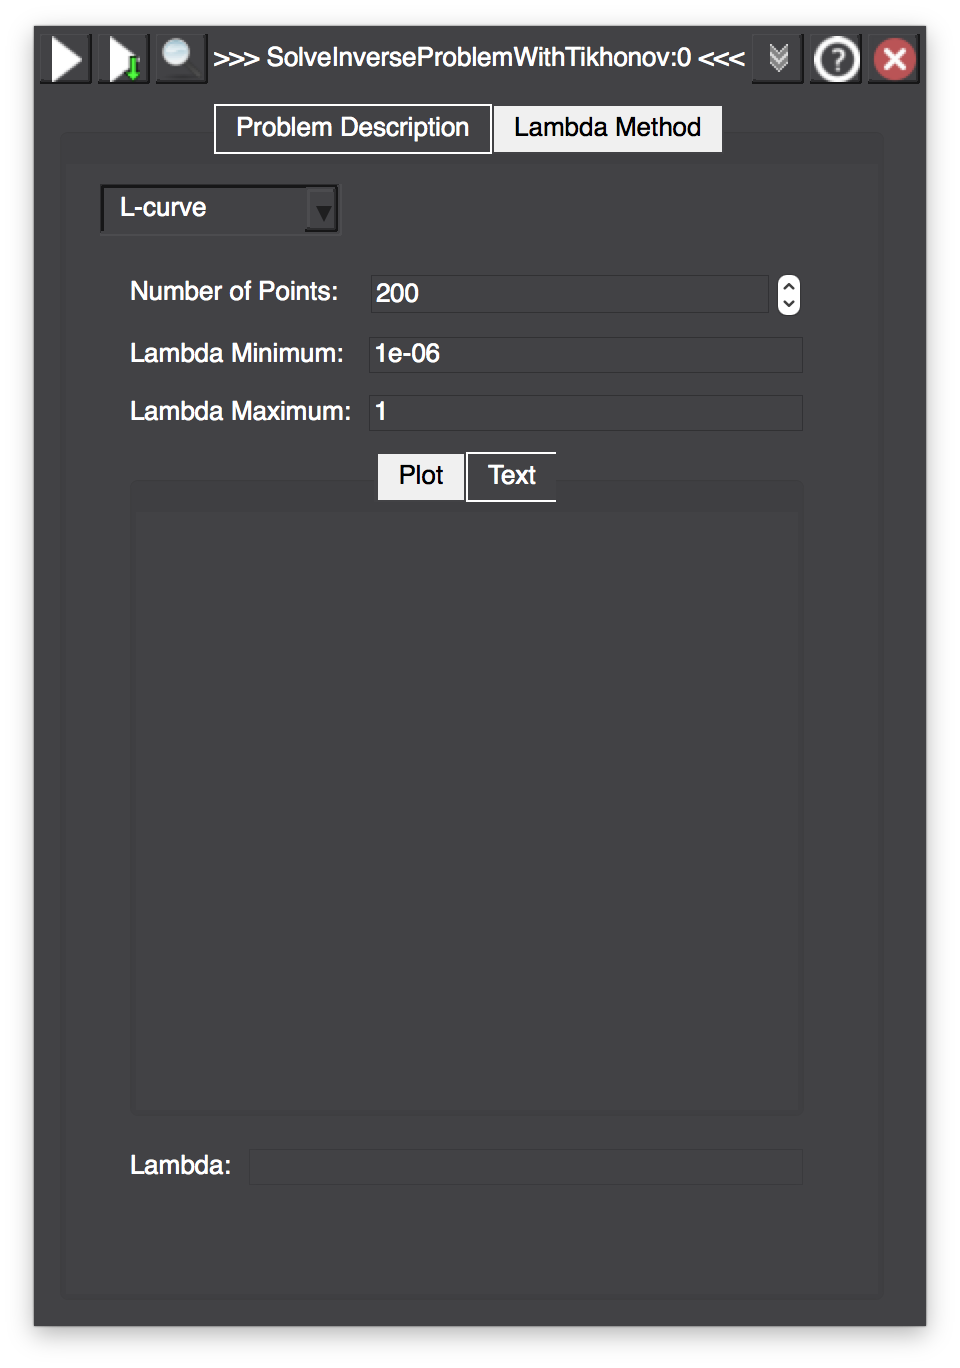
\includegraphics[width=0.45\textwidth]{ECGToolkitGuide_figures/tik3.png}
    \caption{GUI from revised Tikhonov module. Left: problem description. Right: Lambda selection method {\tt SolveInverseProblemWithTikhonov}.}
    \label{fig:tik_module_gui}
    \end{center}
    \end{figure}

    \noindent{\bf Problem Description:}

    There are two formulations for the solutions of least squares problem in \autoref{eq:inverseSec_tik_problem}.
    These are the overdetermined formulation:
    \begin{center}
    \begin{eqnarray}
        \hat{x}   &=& \left(A^T P^TPA + \lambda^{2}R^TR\right)^{-1} A^T P^TP Y,
    \label{eq:inverseSec_TikhonovSolutions1}
    \end{eqnarray}
    \end{center}
    and the underdetermined:
    \begin{center}
    \begin{eqnarray}
        \hat{x}  &=& (R^TR)^{-1} A^T \left( A(R^TR)^{-1}A^T + \lambda^2 (P^TP)^{-1}  \right)^{-1}Y.
    \label{eq:inverseSec_TikhonovSolutions2}
    \end{eqnarray}
    \end{center}
    The difference between these two formulations is computational.
    It can be observed from equations \ref{eq:inverseSec_TikhonovSolutions1} and \ref{eq:inverseSec_TikhonovSolutions2} that the size of the inverse matrix that needs to be computed is $N$ in the overdetermined case and $M$ in the underdetermined.
    Thus, when the number of ECG measurements is smaller than the number of sources on the heart ($N<M$), it is computationally desirable to use \autoref{eq:inverseSec_TikhonovSolutions1}.
    On the other hand, if the number of ECG measurements is larger than the number of sources ($N>M$), it is preferable to use \autoref{eq:inverseSec_TikhonovSolutions2}.
    \href{http://scirundocwiki.sci.utah.edu/SCIRunDocs/index.php/CIBC:Documentation:SCIRun:Reference:BioPSE:SolveInverseProblemWithTikhonov}{{\tt SolveInverseProblemWithTikhonov}} is prepared to use either formulation upon request of the user or choose it automatically based on the size of the forward matrix.
    To choose the desired option, the user must select the appropriate radial button in the ``Regularization Formulation'' option within the  ``Problem Description'' panel.

    The ``Problem Description'' panel also allows to modify how the source and sensor weight matrices ($R$ and $P$) are defined.
    As can be observed in equations \ref{eq:inverseSec_TikhonovSolutions1} and \ref{eq:inverseSec_TikhonovSolutions2}, these two matrices appear in quadratic form. For this reason, many users might prefer to define them in the quadratic form (i.e. $R^2=R^TR$ and $C^2=C^TC$).
    \href{http://scirundocwiki.sci.utah.edu/SCIRunDocs/index.php/CIBC:Documentation:SCIRun:Reference:BioPSE:SolveInverseProblemWithTikhonov}{{\tt SolveInverseProblemWithTikhonov}} allows users to change the default definition of these input matrices to the squared form by selecting the appropriate radial buttons in the ``Constraint Matrices'' options within the  ``Problem Description'' panel.


    \noindent{\bf Lambda Method:}

    The solutions to the Tikhonov regularization problem depend on the selection of the regularization parameter ($\lambda$).
    There are multiple approaches in the literature that allow for its selection.
    \href{http://scirundocwiki.sci.utah.edu/SCIRunDocs/index.php/CIBC:Documentation:SCIRun:Reference:BioPSE:SolveInverseProblemWithTikhonov}{{\tt SolveInverseProblemWithTikhonov}} is currently implemented so that the user can choose between a direct entry, selection using a slider and the L-curve method, described in Sec.~\ref{sec:math_regparam}.
    These methods can be found by selecting the appropriate option in the drop-down menu within the ``Lambda Method'' panel.


    \begin{figure}
        \begin{center}
        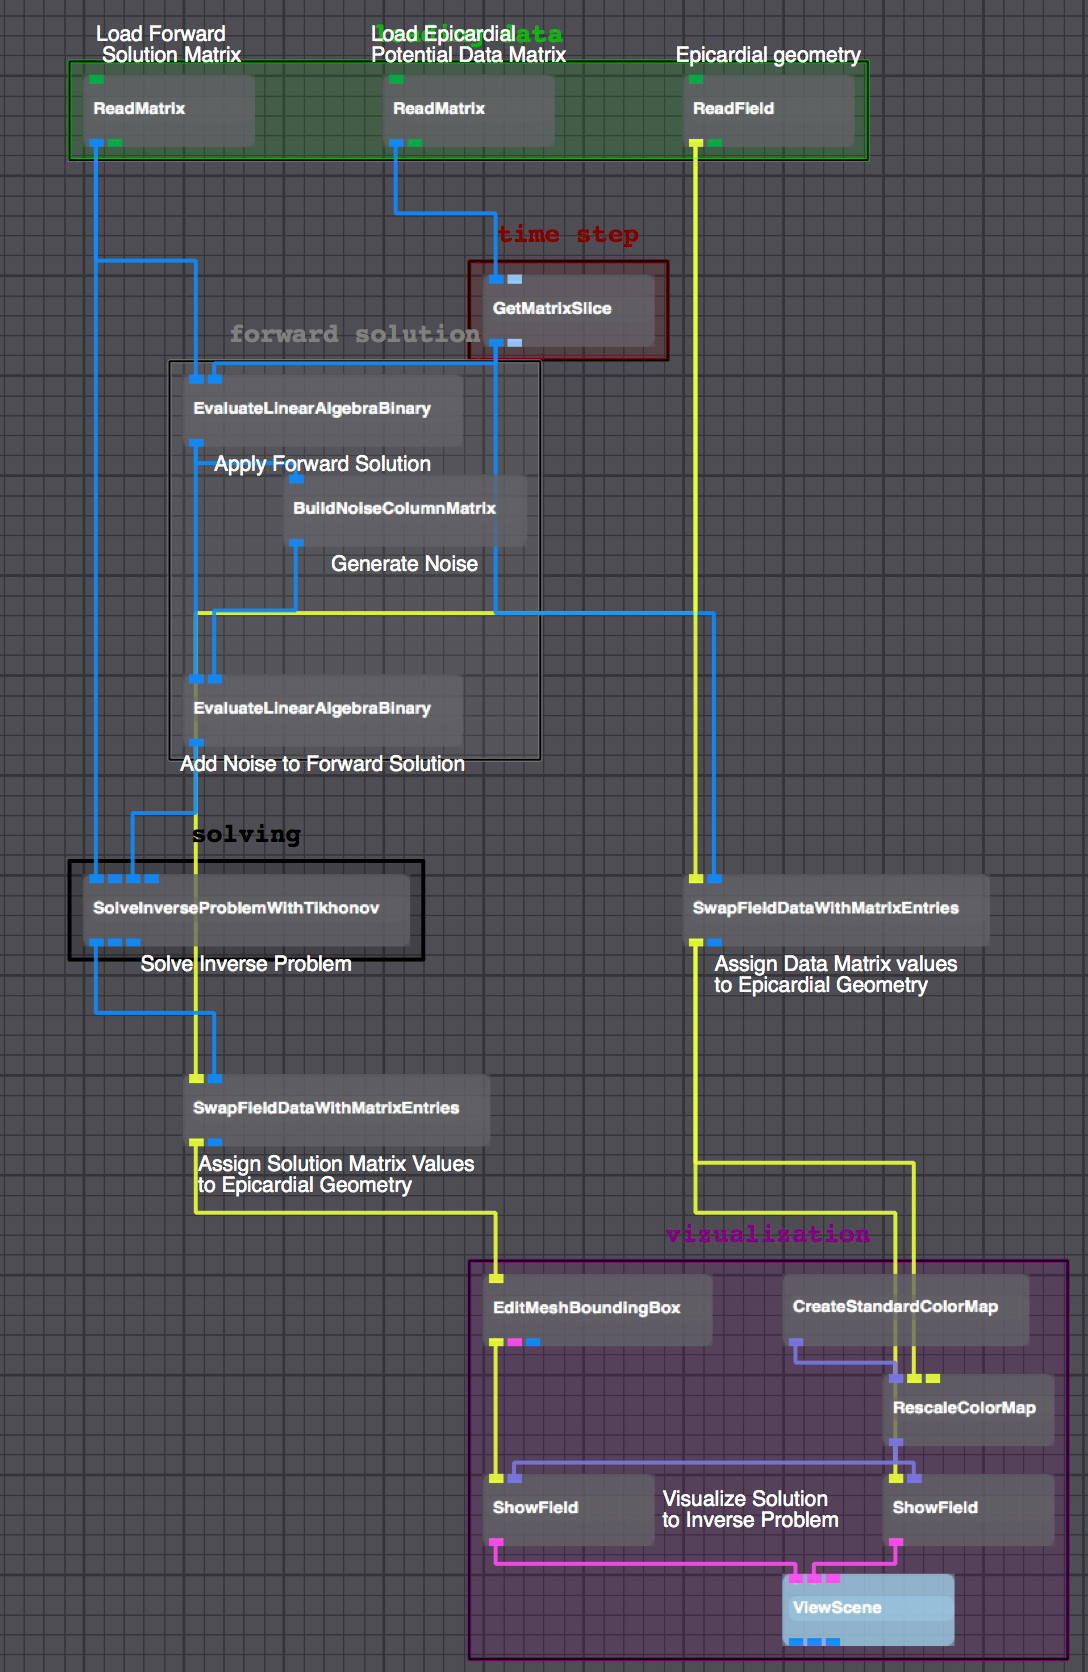
\includegraphics[width=0.9\textwidth]{ECGToolkitGuide_figures/TikhonovNetwork.png}
        \caption{The SCIRun network for the Tikhonov inverse solution example.}
        \label{TikhonovNetworkExample}
        \end{center}
    \end{figure}




\subsection{Tikhonov SVD Method}

    The Tikhonov SVD method effectively solves the same least squares problem as the Tikhonov method described above.
    The difference between these two implementations is computational.
    The \href{http://scirundocwiki.sci.utah.edu/SCIRunDocs/index.php5/CIBC:Documentation:SCIRun:Reference:BioPSE:SolveInverseProblemWithTikhonovSVD}{{\tt SolveInverseProblemWithTikhonovSVD}} module uses the following formulation to solve the least-squares problem:
    \begin{center}
    \begin{eqnarray}
        \hat{X}   &=& \sum_{k=1}^K \frac{\sigma_k}{\lambda^2 + \sigma_k^2} v_k u_k^T Y,
    \label{eq:inverseSec_TikhonovSolutions1}
    \end{eqnarray}
    \end{center}
    where $Y$ are the ECG measurements, $X$ are the unknown potentials on the heart, $\lambda$ is the regularization parameter and $\sigma_k$, $u_k$ and $v_k$ are the singular values, left and right singular vectors of the forward matrix $A$ and $K$ is its rank.

    The \href{http://scirundocwiki.sci.utah.edu/SCIRunDocs/index.php5/CIBC:Documentation:SCIRun:Reference:BioPSE:SolveInverseProblemWithTikhonovSVD}{{\tt SolveInverseProblemWithTikhonovSVD}} module is shown in \autoref{fig:tik_moduleSVD}.
    \begin{figure}
        \begin{center}
        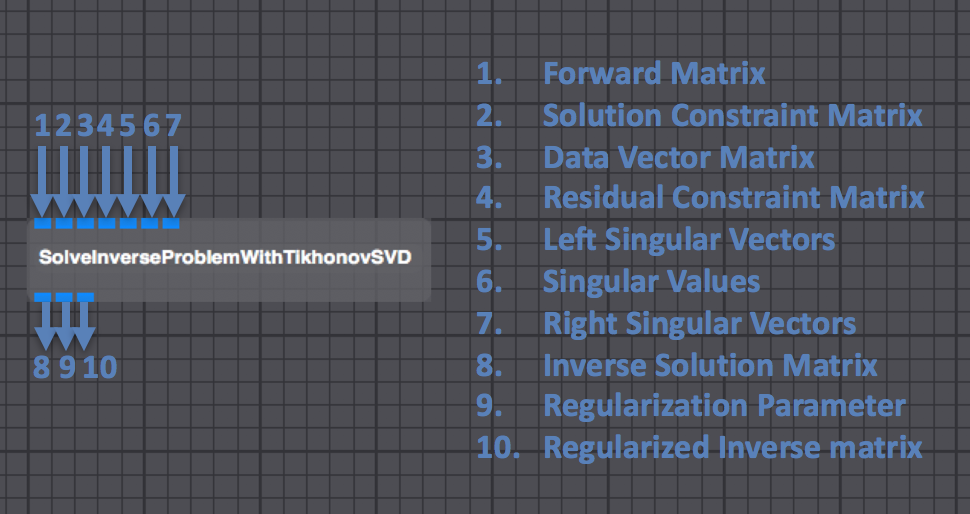
\includegraphics[width=0.7\textwidth]{ECGToolkitGuide_figures/TikhonovSVD_module.png}
        \caption{Revised TikhonovSVD module: {\tt SolveInverseProblemWithTikhonovSVD}.  }
        \label{fig:tik_moduleSVD}
        \end{center}
    \end{figure}
    The inputs and outputs of this module are a superset of \href{http://scirundocwiki.sci.utah.edu/SCIRunDocs/index.php/CIBC:Documentation:SCIRun:Reference:BioPSE:SolveInverseProblemWithTikhonov}{{\tt SolveInverseProblemWithTikhonov}}.
    The new additions permit the user to use pre-computed singular values and vectors of the forward matrix.
    \noindent{\bf Inputs:}
    \begin{enumerate}
        \item Forward Matrix ($A\in\Re^{N,M}$)
        \item Weights in Source Space ($R\in\Re^{L,M}$ or squared $R^2\in\Re^{M,M}$ o)
        \item Measured Potentials ($Y\in\Re^{N,T}$)
        \item Weights in Sensor Space ($P\in\Re^{F,N}$ or squared $P^2\in\Re^{N,N}$)
        \item Left Singular Vectors ($U\in\Re^{N,N}$ )
        \item Singular Values ($S\in\Re^{K,K}$ or in vector form $s\in\Re^{K,1}$)
        \item Right Singular Vectors ($V\in\Re^{M,M}$),
    \end{enumerate}
    {\bf Outputs:}
     \begin{enumerate}
        \item Inverse Solution ($X\in\Re^{M,T}$)
        \item Regularization Parameter ($\lambda$)
        \item Regularized Inverse ($G\in\Re^{M,N}$)
    \end{enumerate}

    \subsubsection{Options and Modes of Operation}

    The options allowed in \href{http://scirundocwiki.sci.utah.edu/SCIRunDocs/index.php5/CIBC:Documentation:SCIRun:Reference:BioPSE:SolveInverseProblemWithTikhonovSVD}{{\tt SolveInverseProblemWithTikhonovSVD}} include the use of a pre-computed singular value decomposition of the forward matrix and the method to select the regularization parameter $\lambda$.

    \noindent{\bf Pre-computed Singular Value Decompositions}

    When needed, \href{http://scirundocwiki.sci.utah.edu/SCIRunDocs/index.php5/CIBC:Documentation:SCIRun:Reference:BioPSE:SolveInverseProblemWithTikhonovSVD}{{\tt SolveInverseProblemWithTikhonovSVD}} automatically computes a Singular Value Decomposition of the input forward matrix using sub-routines found in the Eigen library.
    However, the module is also prepared to use a pre-computed singular value decomposition.
    This option is selected by connecting ALL the input ports of the left and right singular vectors and singular values (ports 5, 6 and 7).
    In this case, the algorithm skips the computation of the SVD and uses the provided matrices.

    \noindent{\bf Lambda Method}

    The solutions to the TikhonovSVD regularization problem depend on the selection of the regularization parameter ($\lambda$).
    There are multiple approaches in the literature that allow for its selection.
    \href{http://scirundocwiki.sci.utah.edu/SCIRunDocs/index.php5/CIBC:Documentation:SCIRun:Reference:BioPSE:SolveInverseProblemWithTikhonovSVD}{{\tt SolveInverseProblemWithTikhonovSVD}} is currently implemented so that the user can choose between a direct entry, selection using a slider and the L-curve method, described in Sec.~\ref{sec:math_regparam}.
    These methods can be found by selecting the appropriate option in the drop-down menu within the ``Lambda Method'' panel as done in \href{http://scirundocwiki.sci.utah.edu/SCIRunDocs/index.php/CIBC:Documentation:SCIRun:Reference:BioPSE:SolveInverseProblemWithTikhonov}{{\tt SolveInverseProblemWithTikhonov}} (see \autoref{fig:tik_module_gui}).


    \begin{figure}
        \begin{center}
        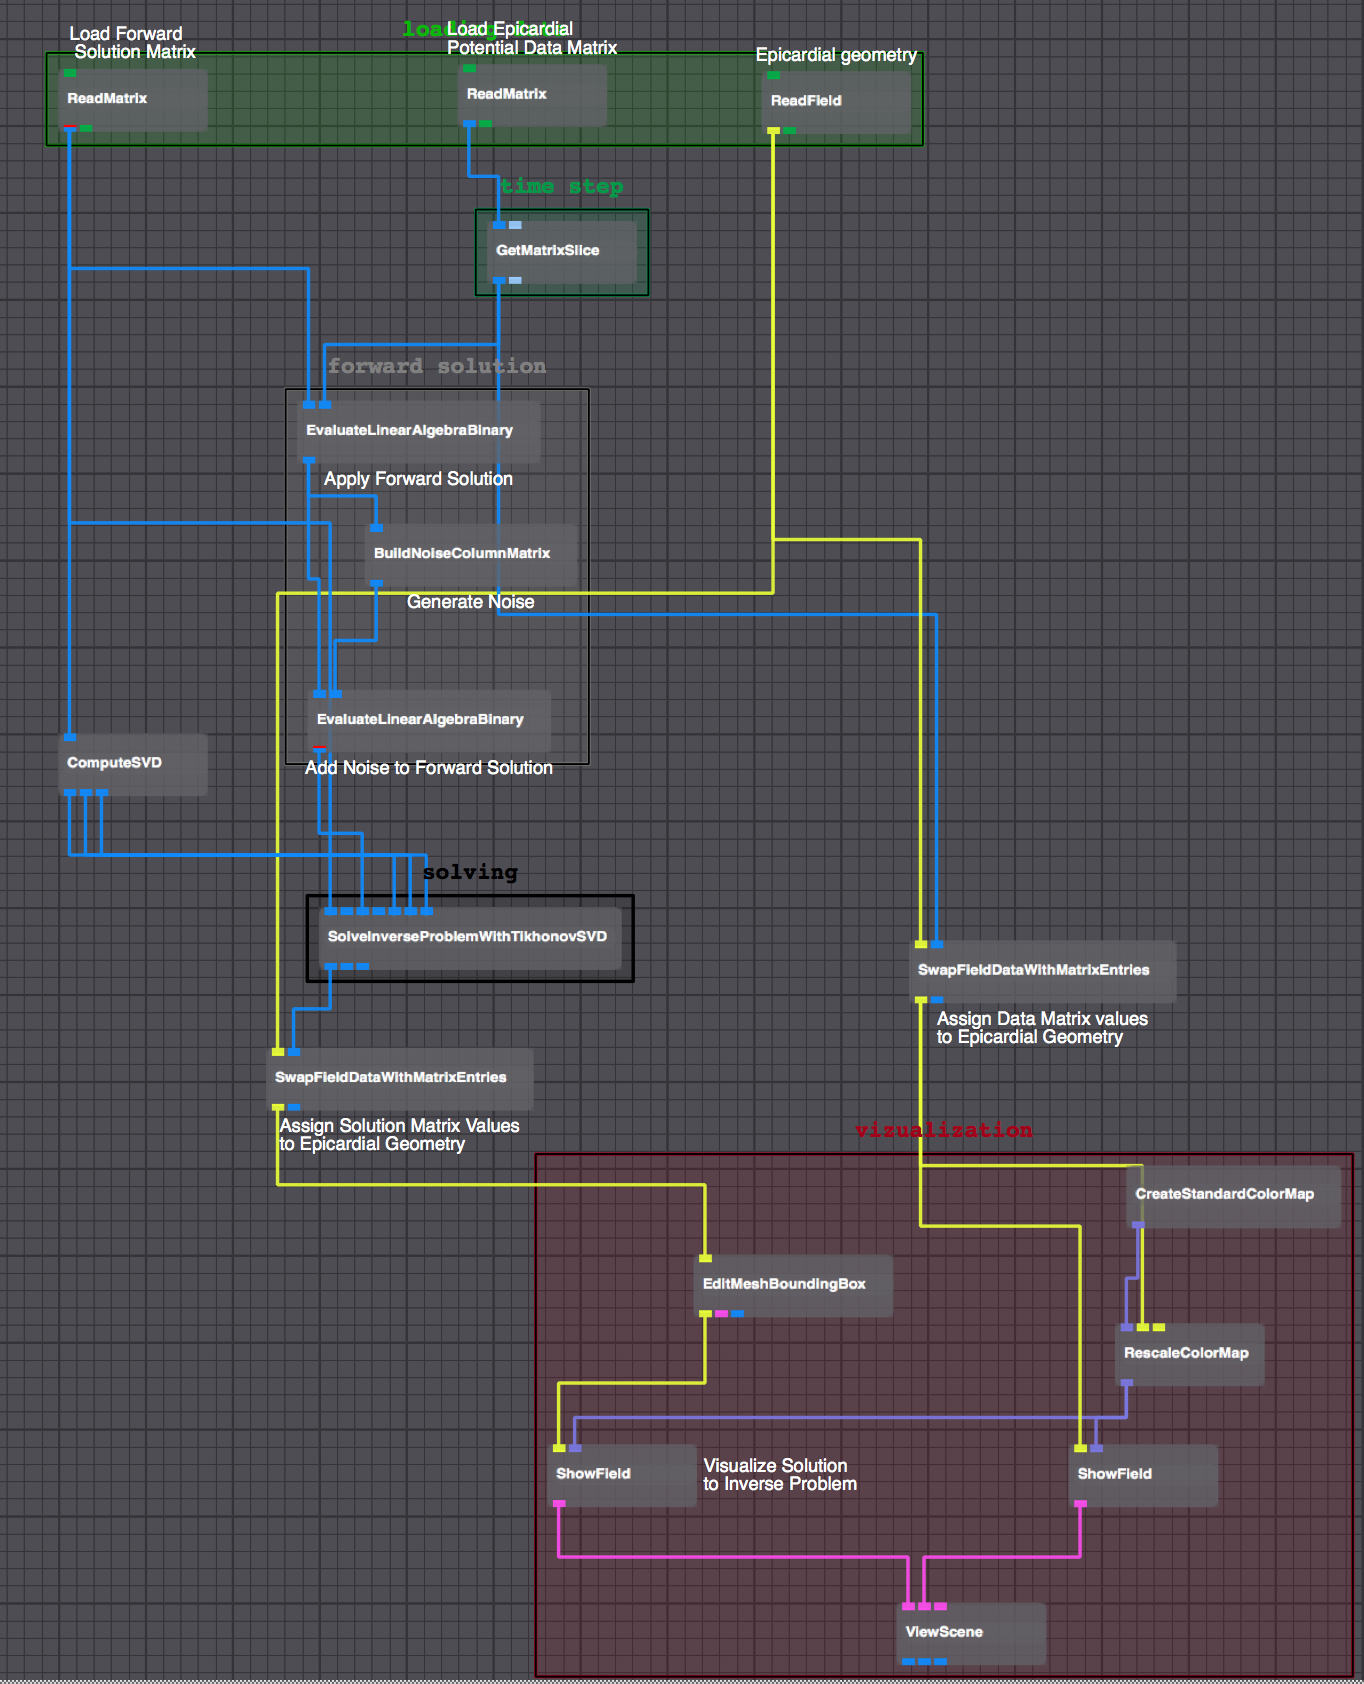
\includegraphics[width=0.9\textwidth]{ECGToolkitGuide_figures/TikhonovSVDNetwork.png}
        \caption{The SCIRun network for the TikhonovSVD inverse solution example.}
        \label{fig:TikhonovNetworkExampleSVD}
        \end{center}
    \end{figure}



\subsection{Truncated SVD Method (TSVD)}

    The truncated SVD method solves the classical least-squares problem with a low-rank approximation of the forward matrix.
    Solutions to this method require the decomposition of the forward matrix $A$ into its left singular vectors $U$, the right singular vetors $V$ and the corresponding singular values $S$.
    Then, these are computed following the formula:
    \begin{center}
    \begin{eqnarray}
        \hat{X}   &=& \sum_{k=1}^Q \frac{1}{\sigma_k} v_k u_k^T Y,
    \label{eq:inverseSec_TikhonovSolutions1}
    \end{eqnarray}
    \end{center}
    where $Y$ are the ECG measurements, $X$ are the unknown potentials on the heart, $\lambda$ is the regularization parameter and $\sigma_k$, $u_k$ and $v_k$ are the singular values, left and right singular vectors of the forward matrix $A$ and $Q$ is the truncation point.

    The module \href{http://scirundocwiki.sci.utah.edu/SCIRunDocs/index.php5/CIBC:Documentation:SCIRun:Reference:BioPSE:SolveInverseProblemWithTSVD}{{\tt SolveInverseProblemWithTSVD}} is shown along its inputs and outputs in \autoref{fig:TSVD_module}
    \begin{figure}
        \begin{center}
        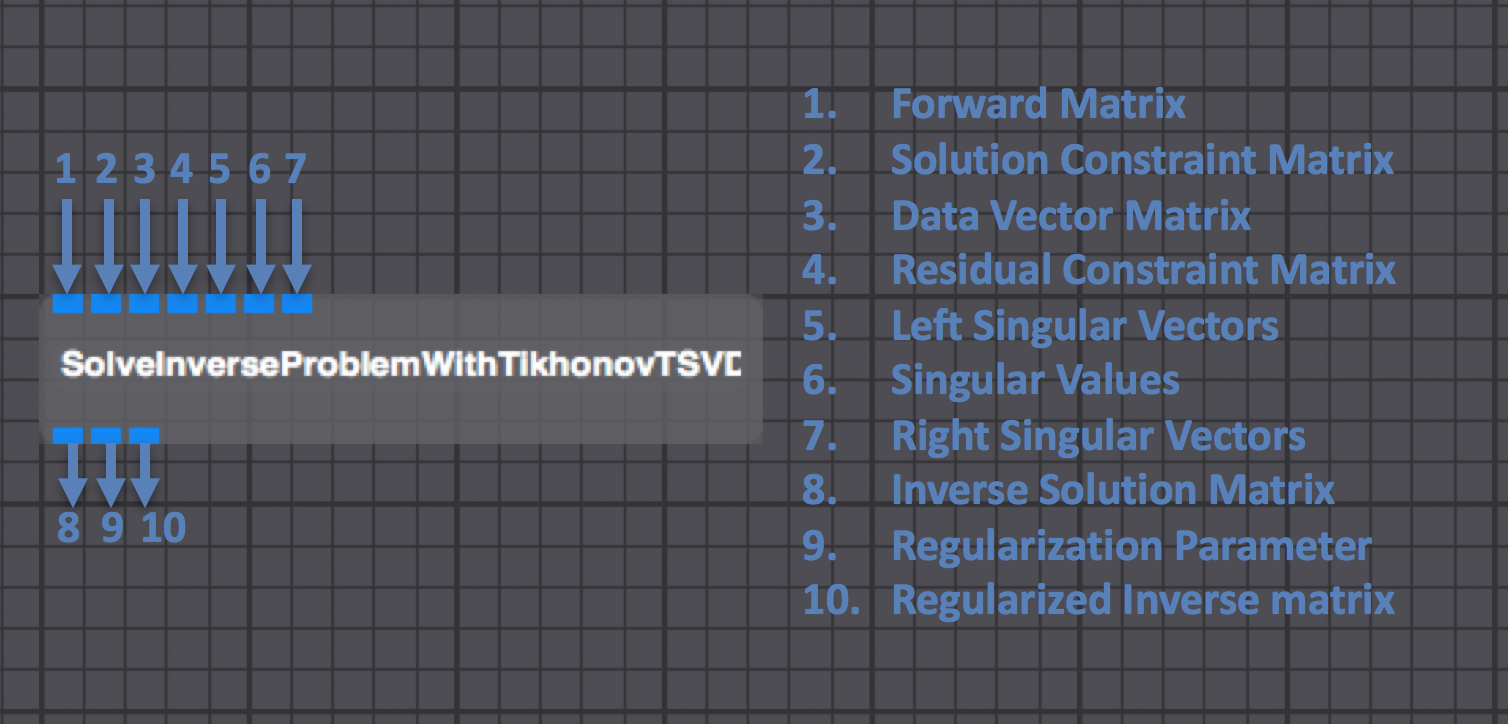
\includegraphics[width=0.7\textwidth]{ECGToolkitGuide_figures/TSVD_module.png}
        \caption{Revised TSVD module: {\tt SolveInverseProblemWithTSVD}.  }
        \label{fig:tik_moduleSVD}
        \end{center}
    \end{figure}
    The inputs and outputs of this module are a superset of \href{http://scirundocwiki.sci.utah.edu/SCIRunDocs/index.php/CIBC:Documentation:SCIRun:Reference:BioPSE:SolveInverseProblemWithTikhonov}{{\tt SolveInverseProblemWithTikhonov}}.
    The new additions permit the user to use pre-computed singular values and vectors of the forward matrix.
    \noindent{\bf Inputs:}
    \begin{enumerate}
        \item Forward Matrix ($A\in\Re^{N,M}$)
        \item Weights in Source Space ($R\in\Re^{L,M}$ or squared $R^2\in\Re^{M,M}$ o)
        \item Measured Potentials ($Y\in\Re^{N,T}$)
        \item Weights in Sensor Space ($P\in\Re^{F,N}$ or squared $P^2\in\Re^{N,N}$)
        \item Left Singular Vectors ($U\in\Re^{N,N}$ )
        \item Singular Values ($S\in\Re^{K,K}$ or in vector form $s\in\Re^{K,1}$)
        \item Right Singular Vectors ($V\in\Re^{M,M}$),
    \end{enumerate}
    {\bf Outputs:}
     \begin{enumerate}
        \item Inverse Solution ($X\in\Re^{M,T}$)
        \item Regularization Parameter ($\lambda$)
        \item Regularized Inverse ($G\in\Re^{M,N}$)
    \end{enumerate}


    \subsubsection{Options and Modes of Operation}

    The options allowed in \href{http://scirundocwiki.sci.utah.edu/SCIRunDocs/index.php5/CIBC:Documentation:SCIRun:Reference:BioPSE:SolveInverseProblemWithTikhonovSVD}{{\tt SolveInverseProblemWithTikhonovSVD}} include the use of a pre-computed singular value decomposition of the forward matrix and the method to select the truncation point (or regularization parameter) $Q$.

    \noindent{\bf Pre-computed Singular Value Decompositions}

    When needed, \href{http://scirundocwiki.sci.utah.edu/SCIRunDocs/index.php5/CIBC:Documentation:SCIRun:Reference:BioPSE:SolveInverseProblemWithTSVD}{{\tt SolveInverseProblemWithTSVD}} automatically computes a Singular Value Decomposition of the input forward matrix using sub-routines found in the Eigen library.
    However, the module is also prepared to use a pre-computed singular value decomposition.
    This option is selected by connecting ALL the input ports of the left and right singular vectors and singular values (ports 5, 6 and 7).
    In this case, the algorithm skips the computation of the SVD and uses the provided matrices.

    \noindent{\bf Lambda Method}

    The solutions to the TSVD regularization problem depend on the selection of the regularization parameter ($Q$).
    There are multiple approaches in the literature that allow for its selection.
    \href{http://scirundocwiki.sci.utah.edu/SCIRunDocs/index.php5/CIBC:Documentation:SCIRun:Reference:BioPSE:SolveInverseProblemWithTSVD}{{\tt SolveInverseProblemWithTSVD}} is currently implemented so that the user can choose between a direct entry, selection using a slider and the L-curve method, described in Sec.~\ref{sec:math_regparam}.
    These methods can be found by selecting the appropriate option in the drop-down menu within the ``Lambda Method'' panel as done in \href{http://scirundocwiki.sci.utah.edu/SCIRunDocs/index.php/CIBC:Documentation:SCIRun:Reference:BioPSE:SolveInverseProblemWithTikhonov}{{\tt SolveInverseProblemWithTikhonov}} (see \autoref{fig:tik_module_gui}).


    \begin{figure}
        \begin{center}
        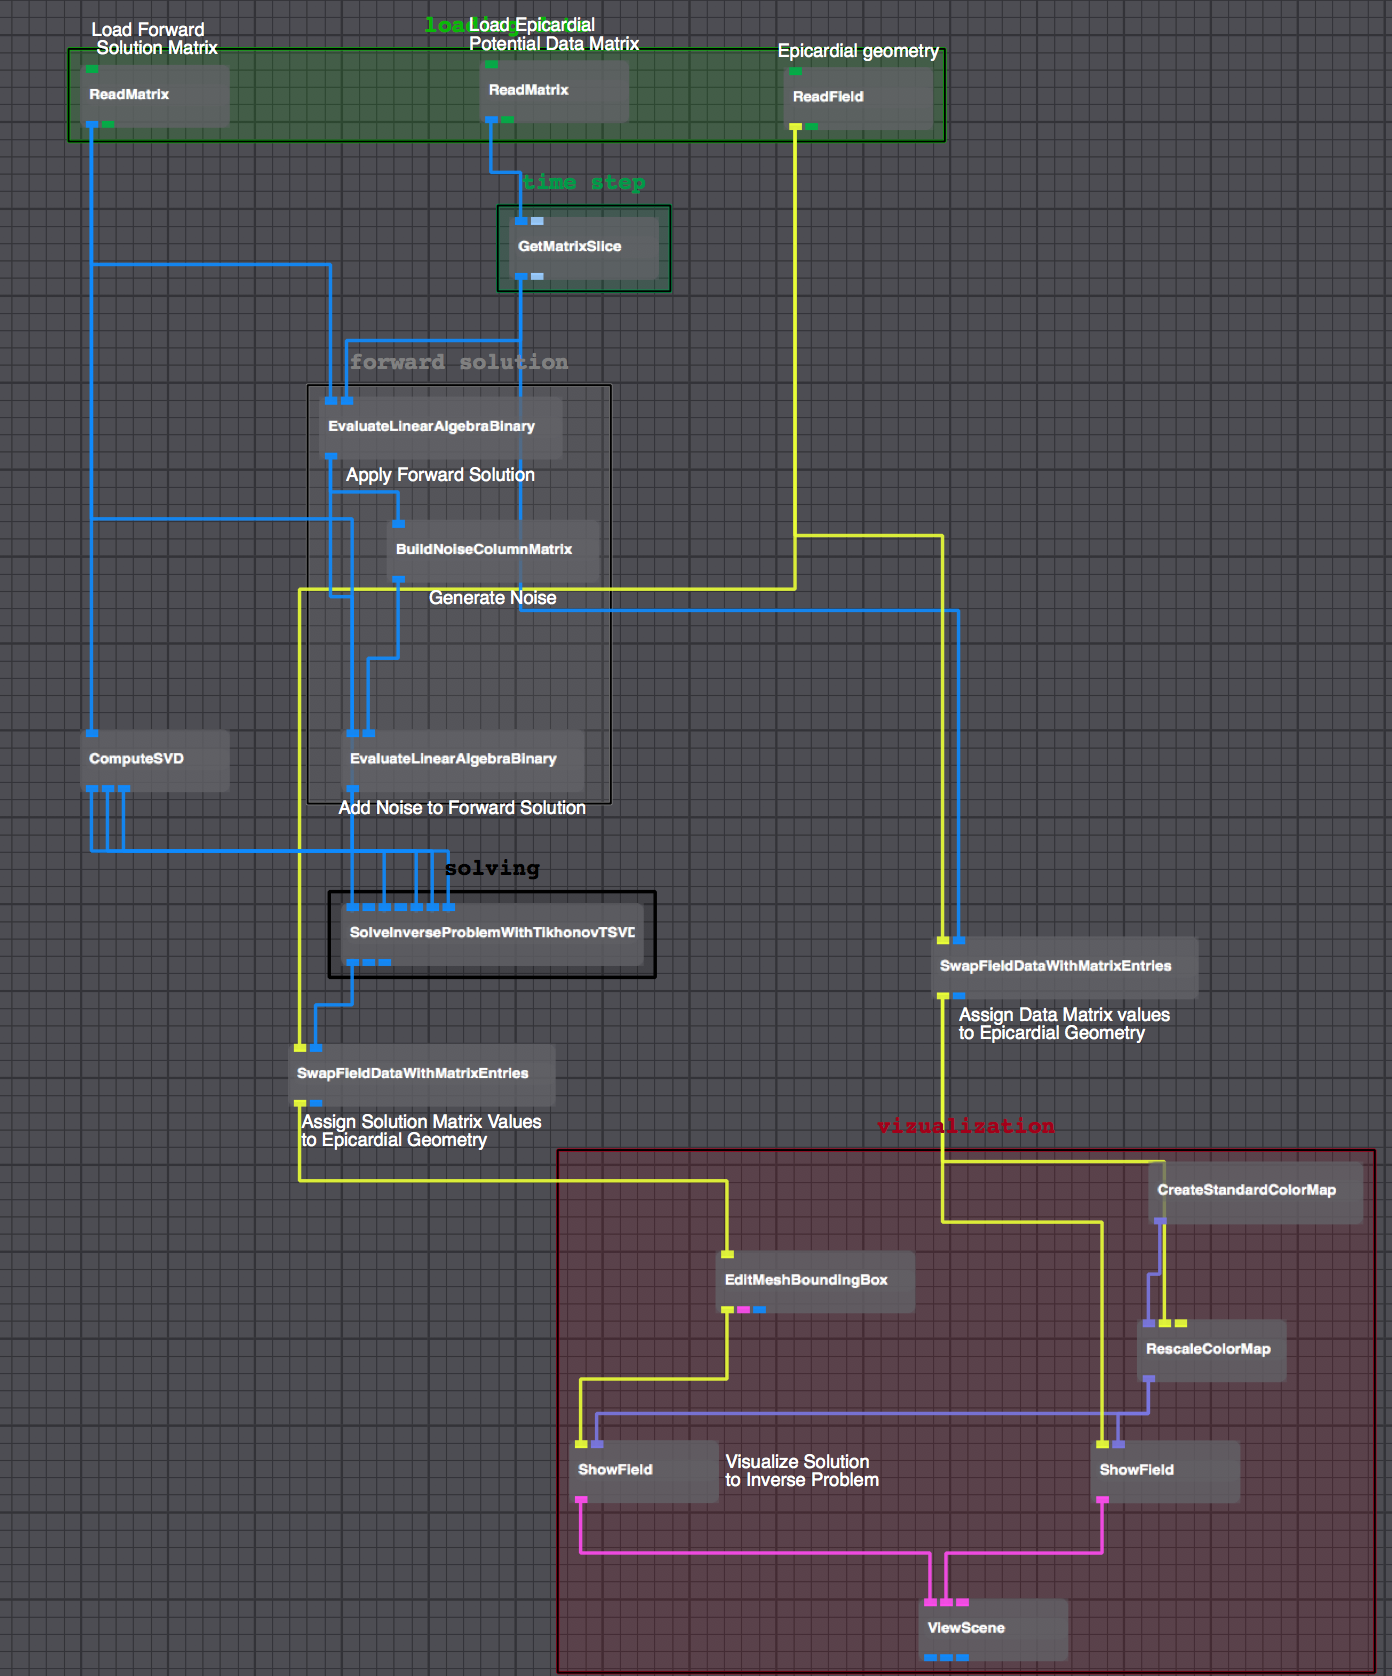
\includegraphics[width=0.9\textwidth]{ECGToolkitGuide_figures/TSVDNetwork.png}
        \caption{The SCIRun network for the TSVD inverse solution example.}
        \label{fig:TSVDNetworkExample}
        \end{center}
    \end{figure}



% \subsection{Total Variation}

%     \subsubsection{Options and Modes of Operation}
   
    
   
\subsection{Method of Fundamental Solutions}

Method of Fundamental Solutions (MFS) is a method to approximate
solutions to partial differential equations, such as Laplace's
equation used in bioelectricity problems.  MFS is similar to BEM in
that it is formulated to take into account boundary conditions and
solutions, but not volumetric ones.  However, MFS is considered
meshless, even though points representing the heart and torso regions
are needed, because the points do not need tessellation, as do BEM and
FEM. In MFS the points representing these regions must be outside the
computational domain, \ie{} in the myocardium and outside the torso,
but as close to the boundary as possible.  Also, unlike BEM and FEM
methods, computing a forward matrix is not necessary.  Instead, the
MFS computes the coefficients representing pericardial potential
values based on analytical evaluation of the potential distribution
and the boundary condition \cite{JDT:Mat77,JDT:Wan2006}.  These
coefficients are are usually solved for with Tikhonov regularization
\cite{JDT:Wan2006,JDT:Joh2018}.  In this toolkit, we implemented MFS
as described by Wang and Rudy \cite{JDT:Wan2006} with the methods to
choose the regularization parameters described by Johnston
\cite{JDT:Joh2018}.  It is implemented in a python library
(`PythonLibrary/MFS\_inverse/mfs\_inverse.py') that can be called from
SCIRun using the InterfaceWithPython module, as shown in
`MSF\_inverse\_Cage.srn5' and `MSF\_inverse\_python.srn5'.

\noindent{\bf Inputs:}
    \begin{enumerate}
        \item Heart boundary ($H\in\Re^{N,3}$)
        \item Torso boundary ($T\in\Re^{M,3}$)
		\item Heart recording points ($P\in\Re^{F,3}$)
		\item Measured Potentials ($Y\in\Re^{K,T}$)
		\item Torso Electrodes ($C$ list of $K$ indices)
        \item options
    \end{enumerate}
    {\bf Outputs:}
     \begin{enumerate}
        \item Inverse Solution ($X\in\Re^{F,T}$)
        \item Regularization Parameter ($\lambda$)
        \item Regularized Curve 
    \end{enumerate}
	

\subsubsection{Options and Modes of Operation}

Options for the algorithm are the scale method (along the normals or
by scaling the point cloud), scale factor, regularization parameter
choosing method \cite{JDT:Joh2018}, lambda range, gamma (for some
techniques).  The implementation has an option to plot the
regularization function.




	
	
    
   
\subsection{Isotropy Method}

    The Isotropy Method is an approach that considers temporal correlations
    to imrove the conditioning of the inverse taken. In SCIRun we have
    implemented this approach with a combination of modules and
    \href{http://scirundocwiki.sci.utah.edu/SCIRunDocs/index.php/CIBC:Documentation:SCIRun:Reference:BioPSE:SolveInverseProblemWithTikhonov}{{\tt
    SolveInverseProblemWithTikhonov}}. Our implementation of the Isotropy
    Method can be found in the example network
    ``potential-based-inverse/greensite-inverse-IsotropyMethod.srn5'',
    shown in \autoref{fig:IsotropyMethod}.

    The network is composed of the standard sections of a simulation
    network to loading data, visualizing and synthesizing the ECG
    measurements. The specific blocks that correspond to the Isotropy
    Method are the ``Temporal Decomposition'', ``solving'' and ``Temporal
    Reconstruction''. Here we describe this blocks in more detail: 



% \subsection{Method of Fundamental Solutions}

%     \subsubsection{Options and Modes of Operation}




    \begin{enumerate}
		\item The {\bf temporal decomposition} block computes the
		singular value decomposition of the input data, truncates the
		right singular vectors (corresponding to time) and projects
		the input data into this lower dimensional space.  
		\item The {\bf solving } block consists on a Tikhonov module
		that solves the inverse problem for the input data projected
		onto the low dimensional temporal space.
		\item The {\bf temporal reconstruction} block, uses the
		truncated right singular vectors from (1) to reconstruct the
		full temporal behavior of the inverse solutions obtained in
		the Tikhonov solver.
    \end{enumerate}

    \subsubsection{Options and Modes of Operation}

    As implemented, the Isotropy Method does not have many options for
    operation. The most important parameter that needs to be determined by
    the user is the truncation point of the right singular vectors, which
    can be accessed in the ``SelectSubMatrix'' module within the ``temporal
    decomposition'' block. The GUI for this module, shown in
    \autoref{fig:IsotropyMethod_gui}, allows to select a submatrix from an
    input matrix. In the case of the isotropy method, the users are only
    interested in the ``end'' parameter from the column range selector
    (lower right entry) since it determined where to truncate the right
    singular vectors.

    This implementation of the Isotropy Method has extra parameters that
    determine the operation of the Tikhonov inverse. These parameters are
    specific to the
    \href{http://scirundocwiki.sci.utah.edu/SCIRunDocs/index.php/CIBC:Documentation:SCIRun:Reference:BioPSE:SolveInverseProblemWithTikhonov}{{\tt
    SolveInverseProblemWithTikhonov}} module and we refer the user to
    \autoref{sec:inverse:tikhonov} for more details.

   \begin{figure}
       \begin{center}
       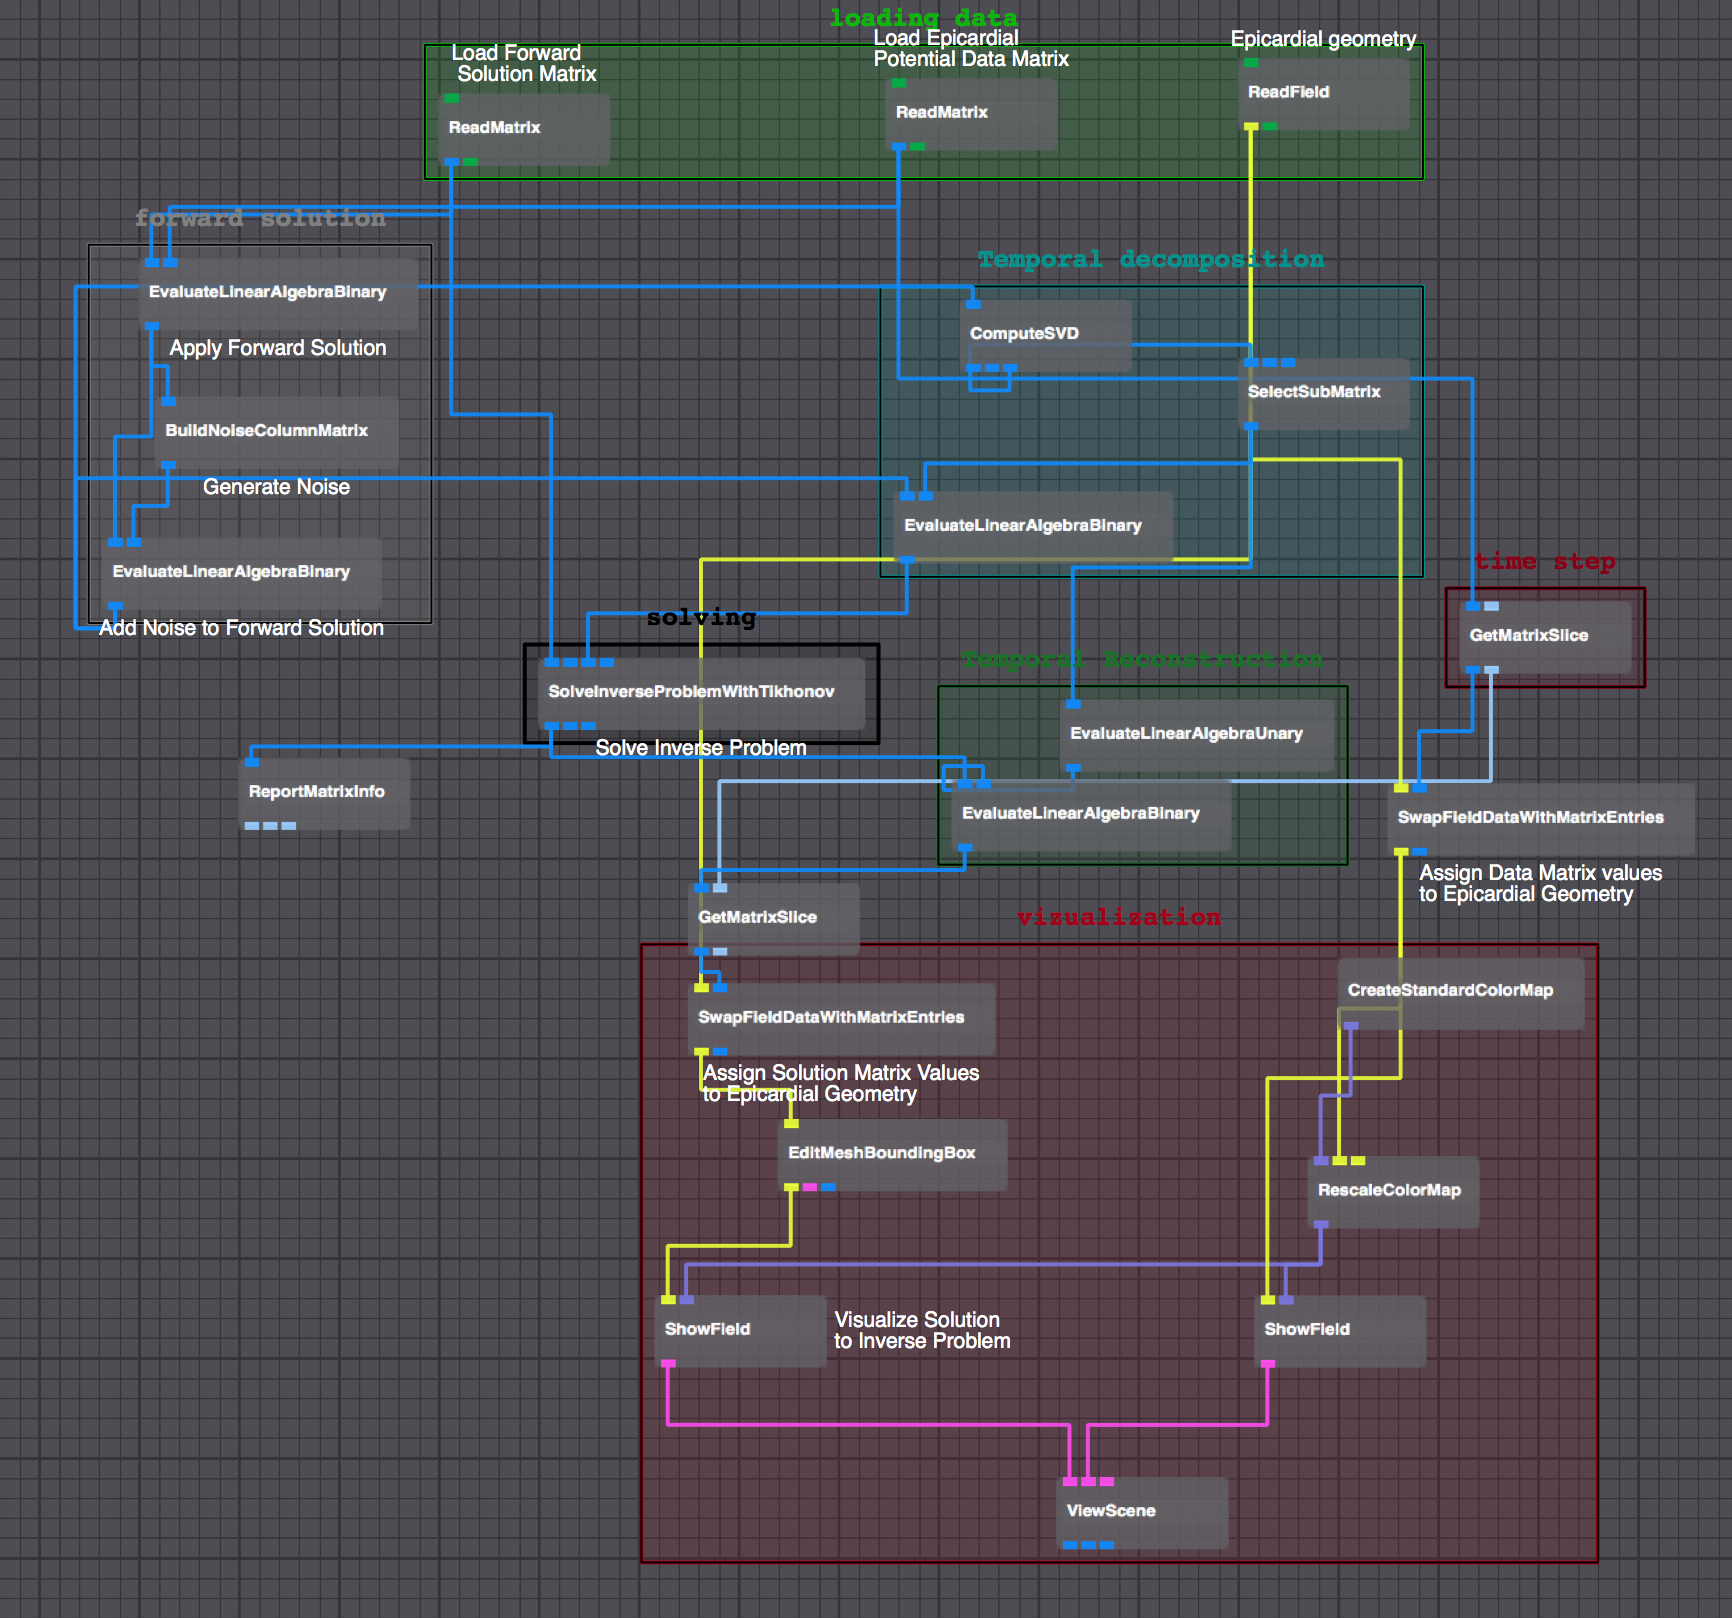
\includegraphics[width=0.9\textwidth]{ECGToolkitGuide_figures/IsotropyMethod_networkExample.png}
       \caption{The SCIRun network for the Isotropy Method inverse solution example.}
       \label{fig:IsotropyMethod}
       \end{center}
   \end{figure}


\subsection{Spline-Based Inverse Method}

    The spline-based inverse method is another approach that takes into account the temporal characteristics of the signal. In this particular case, it projects the input data onto a 1D manifold characterized with a spline \cite{}.
    The current implementation of this method uses the MATLAB-python interface capabilities as well as the implemented inverse methods.
    Similarly to the Isotropy Method, the spline-based inverse is composed of three main blocks ``temporal decomposition'', ``inverse solving'' and ``temporal recontruction''.
    The main difference concerns the temporal decomposition and reconstruction steps, which now are non-linear and involve the estimation fo a 1D manifold.
    In the following, we will describe these three blocks:

    \noindent{\bf Manifold Estimation:}

    \begin{verbatim}
    %		This code implements the inverse solutions pipeline presented in
    %		the paper:
    %	        Erem, Coll-font, Martinez Orellana - 2013 -
    %	        Using Transmural Regularization and Dynamic Modeling
    %	        for Non-Invasive Cardiac Potential Imaging of
    %	        Endocardial Pacing Sites with Imprecise Thoracic Geometry.
    %
    %		Inputs
    %				  i1 - <N,T>double - measured potentials on the torso.
    %				  i2 - <N,M>double - forward matrix.
    %				  i3 - <L,M>double - regularization matrix.
    %				  i4 - <3,1>int - regularization constant params.
    %				                  i4(1) - log10 min lambda.
    %				                  i4(2) - log10 max lambda
    %				                  i4(3) - num lambda.
    %		Outputs
    %				  o1 - <M,T>double - estimated heart potentials.
    \end{verbatim}


    \noindent{\bf Inverse Solution:}
    \begin{verbatim}

    \end{verbatim}

    \begin{figure}
        \begin{center}
        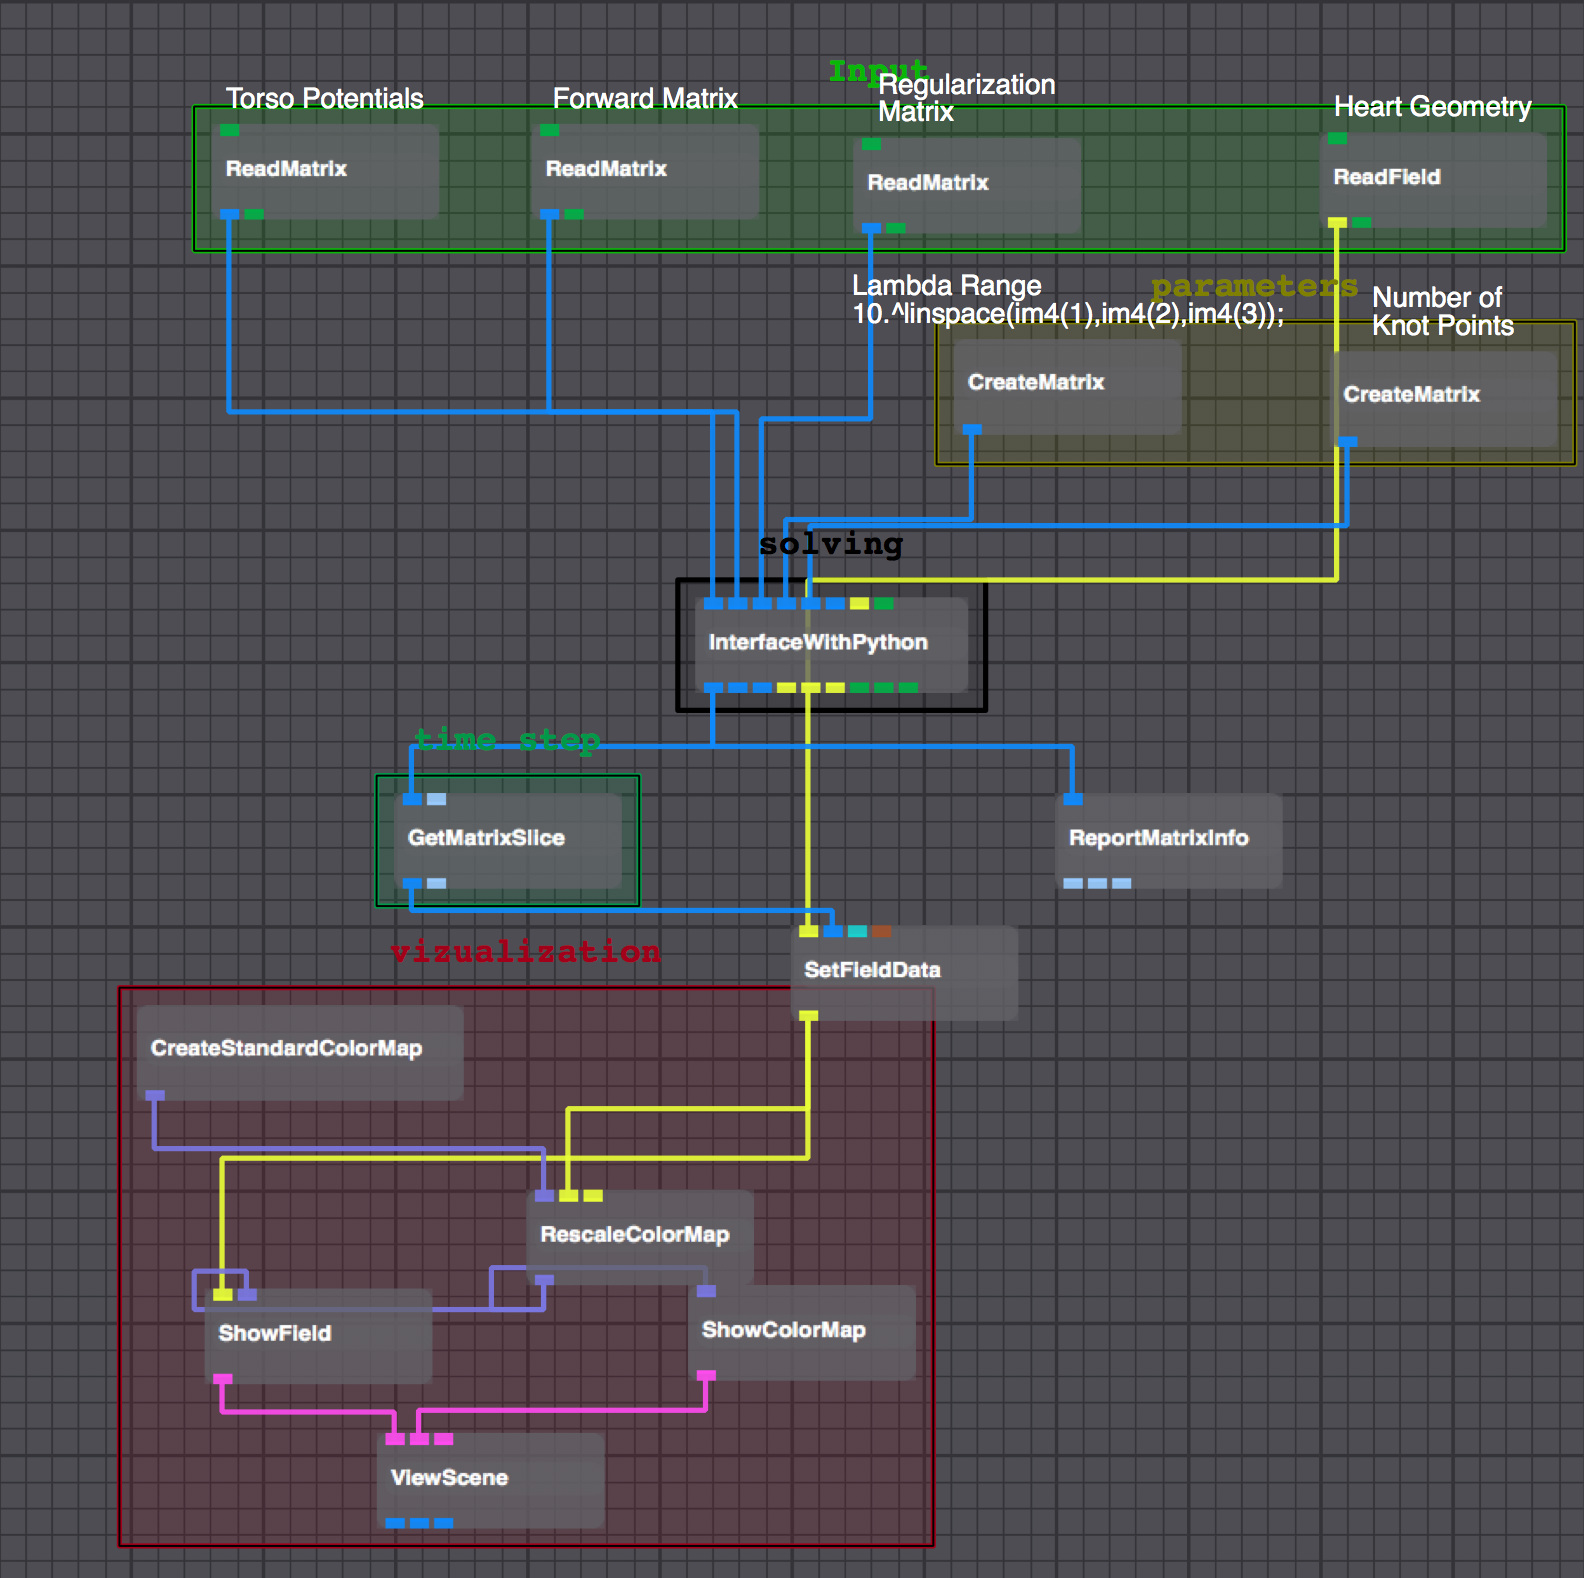
\includegraphics[width=0.9\textwidth]{ECGToolkitGuide_figures/splineInverse_Network.png}
        \caption{The SCIRun network for the Spline-Based Method inverse solution example.}
        \label{fig:splineInverse}
        \end{center}
    \end{figure}



\subsection{Non-Decreasing Inverse Method}

    The Non-Decreasing Inverse Method estimates the transmembrane potentials by solving a constrained Tikhonov problem.
    Thus the function to be optimized over is a standard Tikhonov problem but restricts the solutions to always be non-decreasing.
    Thus, the problem to be solved is:
    \begin{equation}\begin{split}
    		\min_{x(t), t=1\dots T} &\|y(t) - Ax(t)\|_2^2 + \lambda*\|Rx(t)\|_2^2 \\
    		&s.t.\\
      		&\hspace{2cm}x(1) >= minB\\
         	&\hspace{2cm}x(t+1) >= x(t), \hspace{.2cm}t=1\dots T-1\\
         	&\hspace{2cm}x(T) <= maxB
    \end{split}
    \end{equation}
    Where $minB$ and $maxB$ are the minimum and maximum bounds for the TMP.
    For memory efficiency, this problem is implemented with an ADMM solver.

    This model assumes that the electrical sources of the heart model the transmembrane potentials on each node of the geometry. The inputs and ouputs of the MATLAB implementation can be seen here:
    \begin{verbatim}
    %% MESSNARZ INVERSE SCRIPT FOR SCIRUN
    %
    %           (...)
    %			INPUT:
    % 					- A - <N M>double - forward operator of the linear system.
    % 					- R - <H,M>double - regularization matrix.
    % 					- ECG - <N,T>double - Body surface measurements.
    % 					- lambda - double - regularization term.
    % 					- initialx - <M,T>double - initial guess for the TMP
    % 					solution.
    % 					- rho - double - augmented term weight.
    % 					- min_r - double - stopping criteria for the primal
    % 					residual.
    % 					- min_s - double - stopping criteria for the dual residual.
    %					- margin - <2,1>double - minimum and maximum bounds for
    %					the transmembrane potentials.
    % 					- verbose - boolean - print ADMM iteratinons information.
    %
    %			OUTPUT:
    % 					- xk - <M,T>double - estimated TMP.
    % 					- zk - <M,T+1>double - estimated slack variable.
    %           (...)
    %
    \end{verbatim}
    \noindent{\bf Inputs:}
    \begin{enumerate}
        \item Forward Matrix ($A\in\Re^{N,M}$)
        \item Regularization matrix ($R\in\Re^{F,N}$)
        \item Measured Potentials ($Y\in\Re^{N,T}$)
        \item Regularization parameter ($\lambda\in\Re$)
        \item Initial guess for the transmembrane potentials ($X_0\in\Re^{N,1}$ )
        \item ADMM parameters: weight of augmented lagrangian, stopping paramter for primal and dual objectives ($\rho, min_r, min_s \in\Re^{+}$)
        \item Lower and upper bounds (margin) of the transmembrane potentials ($marg\in\Re^2$)
    \end{enumerate}

    \noindent{\bf Outputs:}
    \begin{enumerate}
        \item Heart potentials ($xk\in\Re^{M,T}$ )
    \end{enumerate}

    The resulting potentials have sharp increases of potentials similar to the typically observed in TMPs for most of the nodes on the heart geometry.
    In general, the final solution is insensitive to the initial guess but it will affect the time of convergence.
    The script is set up such that the initial guess for the first lambda is a simple ramp, after each initial guess is the final result of the previous lambda.
    The decision of the correct lambda is done automatically using an L-corner detection.
    This algorithm is implemented as the SCIRUN network shown in \autoref{fig:nonDecreasingNetwork}

    NOTE: This code requires the software package reguTools (http://www.imm.dtu.dk/~pcha/Regutools/) to be incorporated in the default path from MATLAB.

    % % \subsubsection{Options and Modes of Operation}
    % \begin{figure}
    %     \begin{center}
    %     \includegraphics[width=0.9\textwidth]{ECGToolkitGuide_figures/nonDecreasingNetwork.png}
    %     \caption{The SCIRun network for the Non-Decreasing Inverse Method inverse solution example.}
    %     \label{fig:nonDecreasingNetwork}
    %     \end{center}
    % \end{figure}



\subsection{Activation-Based Method}

    The activation-based inverse method solves the inverse problem in electrocardiography through the estimation of the activation times (\emph{i.e.} the depolarization times) on the heart.
    This inverse method assumes that the sources on the heart are modeled with a potentials over time at each node are parameterized  by the time of activation.
    This assumption allows the inverse method to resolve the inverse problem by estimating the activation times at every node on the heart geometry.

    The inverse problem being solved is thus a non-linear optimization problem for which there is no closed-form solution.
    The implementation of the activation-based inverse in SCIRun is done with a Gauss-Newton iterative method that solves:
    \begin{center}
        \begin{eqnarray}
            min_{X} \|Y - A \Phi(\tau, \omega) \|^{2}_{2} + \lambda \| R\Phi(\tau, \omega) \|^{2}_{2},
        \label{eq:inverseSec_actBasedObj}
        \end{eqnarray}
    \end{center}
    where $\Phi(\cdot)$ is the pre-defined temporal waveform at each node and is paramaterized by $\tau$ and $\omega$, which correspond to the time of activation and the slope of the depolarixzation wave respectively.
    $Y$ are the measured body surface potentials, $A$ the forward matrix and $R$ the regularization matrix.

    The inputs and outputs of this inverse method can be observed in the ``InterfaceWithPython'' module in the network example shown in \autoref{fig:activationBasedNetwork} and in the header of the MATLAB implementation:
    \begin{verbatim}
        function tau = ActGaussNewton(A,Y,L,tauinit,lambda,w,minstep)
        % Implements the Gauss-Newton algorithm for solving the activation-based
        % inverse problem of electrocardiography.
        % => minimizes the objective function ||Y-A*X||^2+lambda*||L*X||^2 where
        % X is parameterized by the C^1 polynomial approximation to a step function
        % as explained in "The Depolarization Sequence of the Human Heart Surface
        % Computed from Measured Body Surface Potentials" by Geertjan Huiskamp and
        % Adriaan van Oosterom.
        %
        % Input Variables:
        % A: Forward matrix
        % Y: Observations (columns index time from 1 to T=size(Y,2))
        % L: Regularization matrix (typically a surface Laplacian approximation)
        % lambda: Regularization parameter
        % w: Width parameter in step function approximation
        % tauinit: Initial phase shifts for starting the algorithm
        %
        % Output Variables:
        % tau: Solution phase shifts of the step functions
    \end{verbatim}

    \noindent{\bf Inputs:}
    \begin{enumerate}
        \item Forward Matrix ($A\in\Re^{N,M}$)
        \item Measured Potentials ($Y\in\Re^{N,T}$)
        \item Regularization matrix ($R\in\Re^{F,N}$)
        \item Initial guess for the activation times ($\tau\in\Re^{N,1}$ )
        \item Regularization parameter ($\lambda\in\Re$)
        \item Activation waveform transition width ($\omega\in\Re^{+}$)
        \item Convergence parameter ($\epsilon\in\Re^{+}$)
    \end{enumerate}
    The initial guess is the set of activation times from which the Gauss-Newton algorithm starts pursuing a more suitable inverse solution.
    The transition width controls the number of time samples (not necessarily integer) taken by each source to transition from inactivated to activated in this method.
    The convergence parameter is the minimum norm of the step taken by the iterations within the Gauss-Newton algorithm before the method is deemed to have converged to a suitable solution.

    \noindent{\bf Outputs:}
    \begin{enumerate}
        \item Activation times ($\tau\in\Re^{M,1}$ )
    \end{enumerate}
    The only output of the method is the inverse solution in the form of an array of activation times.

   \begin{figure}
       \begin{center}
       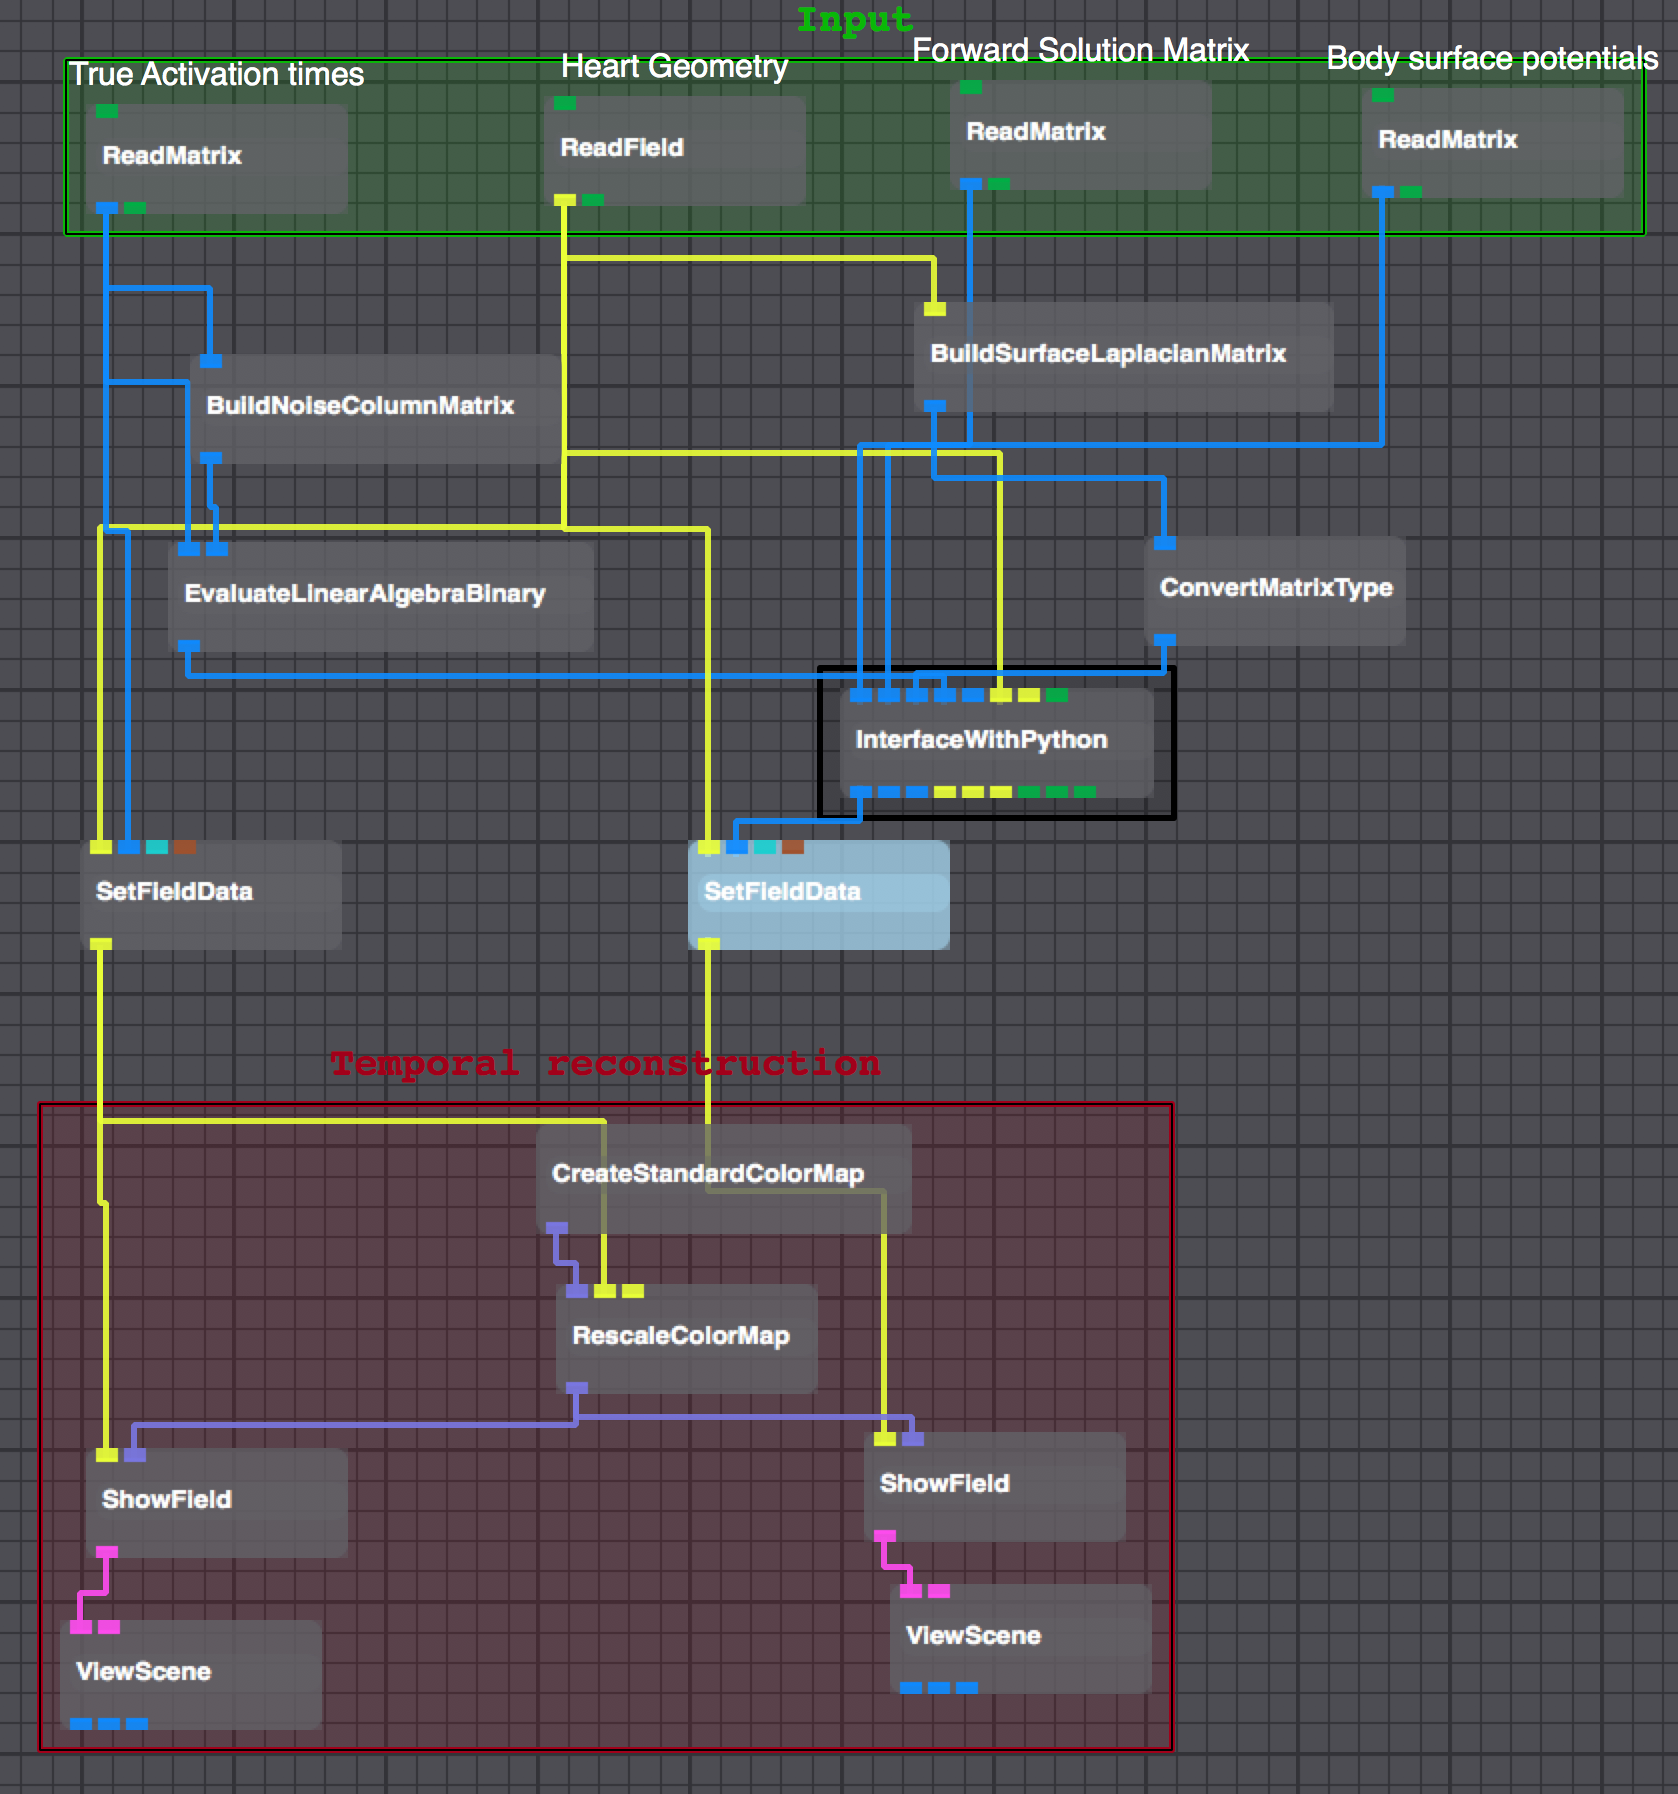
\includegraphics[width=0.9\textwidth]{ECGToolkitGuide_figures/activationBasedNetwork.png}
       \caption{The SCIRun network for the Activation-Based Method inverse solution example.}
       \label{fig:activationBasedNetwork}
       \end{center}
   \end{figure}


\subsection{Wavefront-Based Potential Reconstruction (WBPR)}

    The Wavefront-Based Potential Reconstruction (WBPR) method imposes prior knowledge about the spatial patterns of electric potentials on the heart during the QRS complex to reconstruct an inverse solution.
    This inverse method assumes a source model characterizing the extracellular potentials on the heart surface and introduces a regularization term that imposes them to be similar to a pre-specified shape.

    The inputs and outputs of this inverse method can be observed in the ``InterfaceWithPython'' module in the network example shown in \autoref{fig:WBPRNetwork} and in the header of the MATLAB implementation:
    \begin{verbatim}
    function [x_WBPR_forward,x_WBPR_backward] = WBPR(A,y,heart,first_act,last_act)
    % Function to calculate the WBPR solutions
    % Inputs:
    %   A: forward matrix
    %   y: torso data
    %   heart: heart geometry
    %   first_act: first activated node
    %   last_act: last activated node
    %
    % Outputs:
    %   x_WBPR_forward: inverse solution using forward WBPR
    %   x_WBPR_backward: inverse solution using backward WBPR
    \end{verbatim}

    \noindent{\bf Inputs:}
    \begin{enumerate}
        \item Forward Matrix ($A\in\Re^{N,M}$)
        \item Measured Potentials ($Y\in\Re^{N,T}$)
        \item Heart geometry (struct containing nodes and triangles)
        \item First and last nodes to activate ()
    \end{enumerate}

    \noindent{\bf Outputs:}
    \begin{enumerate}
        \item forward WBPR solution ($X_f\in\Re^{M,T}$ )
        \item backward WBPR solution ($X_b\in\Re^{M,T}$ )
    \end{enumerate}
    As output, WBPR produces two inverse solutions. The procedure by which the inverse solutions are obtained may be run both forward and backward in time. Therefore, the ``forward WBPR'' solution is that obtained by applying the method starting from the earliest sample time and ending at the latest. On the other hand, the ``backward WBPR'' solution is obtained by starting from the latest sample time and traversing the samples in reverse until ending at the earliest.

    NOTE: This code requires the software package reguTools (http://www.imm.dtu.dk/~pcha/Regutools/) to be incorporated in the default path from MATLAB.

    \begin{figure}
        \begin{center}
        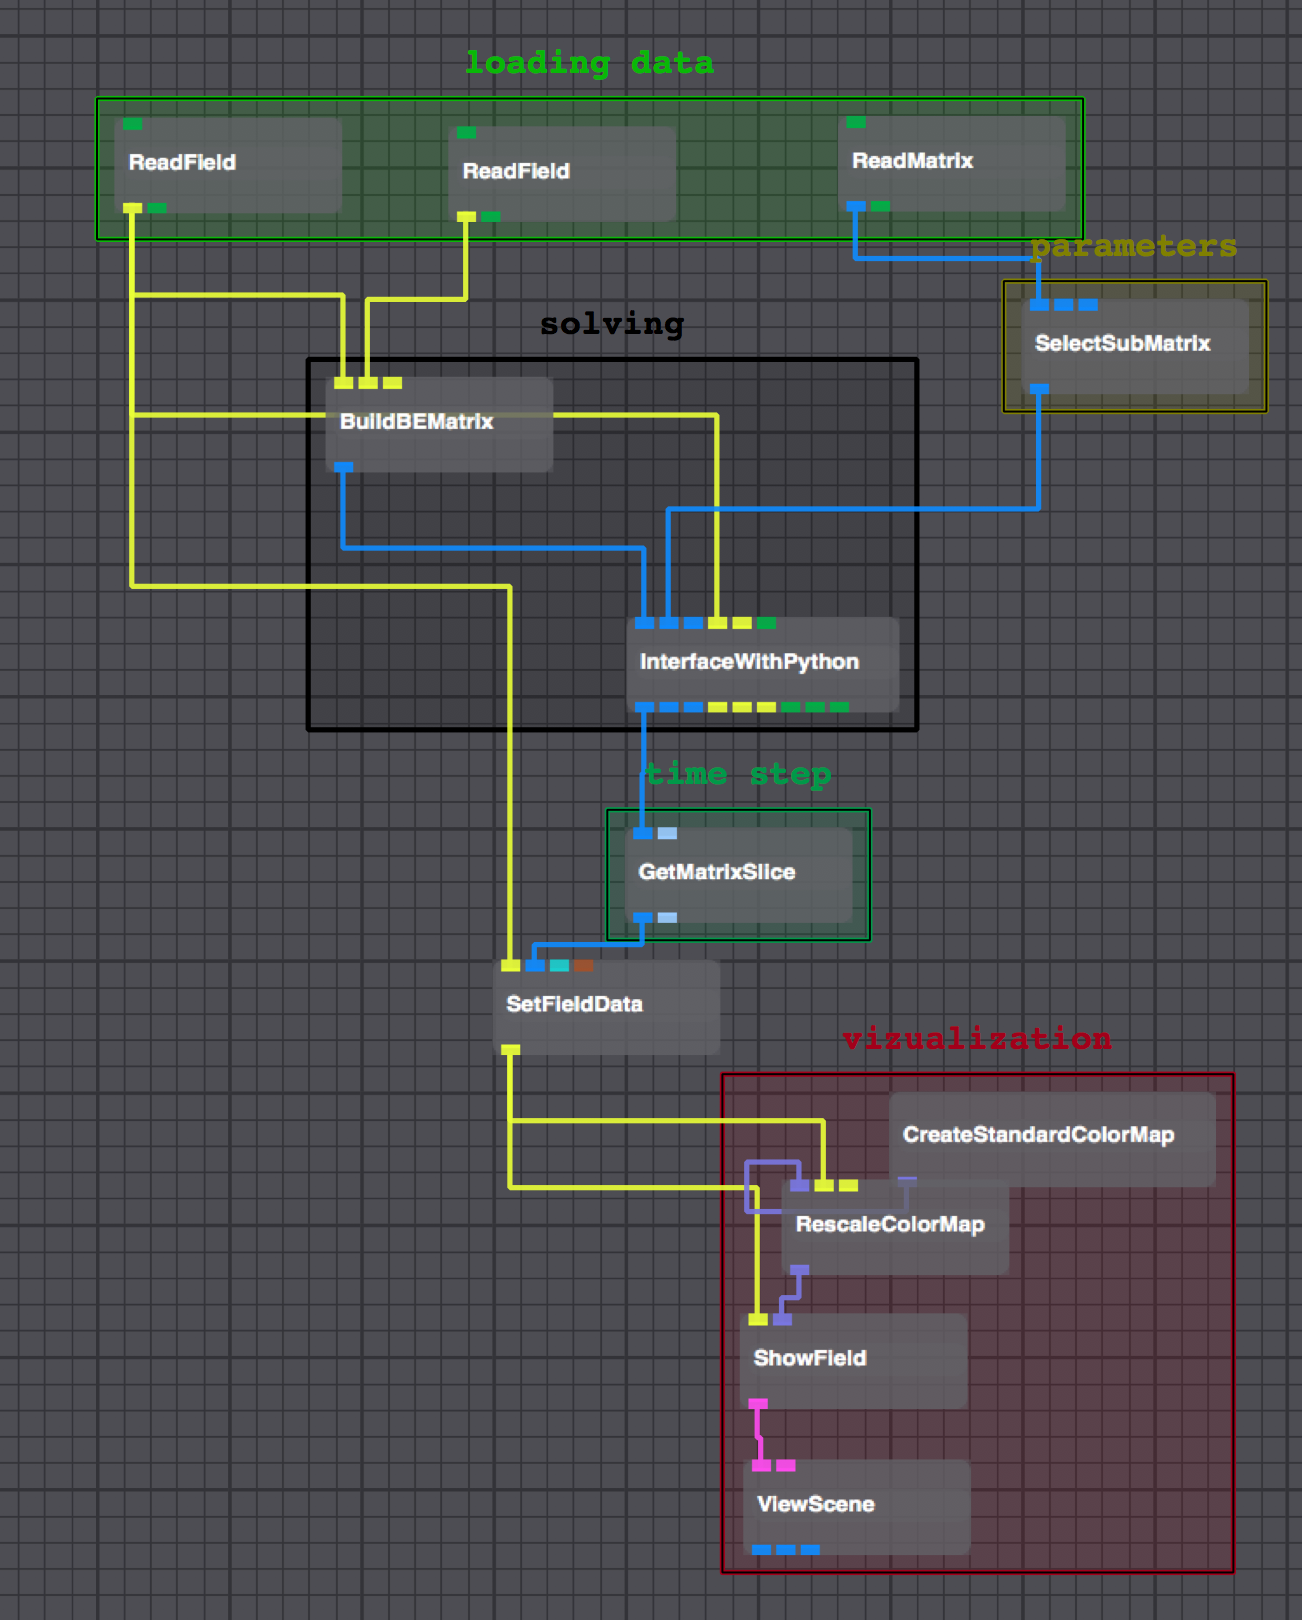
\includegraphics[width=0.9\textwidth]{ECGToolkitGuide_figures/WBPRNetwork.png}
        \caption{The SCIRun network for the WBPR Method inverse solution example.}
        \label{fig:WBPRNetwork}
        \end{center}
    \end{figure}


\chapter{Inverse Solutions}
\label{ch:inv}

\section{Overview}

The inverse problem of electrocardiography is to find suitable electrical source parameters on the heart that adequately describe the observed body surface potentials. Regularization is typically employed in solution methods to reduce the sensitivity of the problem to relatively small errors in the observed body surface potentials, thereby stabilizing it. As a result, solution methods may be supplied body surface potentials, a forward model, and method-specific regularization parameters as input. Specific use of each method is described below. As output, modules primarily produce the resulting solution with extra outputs, depending on the specific method.

\section{Module Descriptions for Inverse Solution Methods}

%%%%%%%%%%%%%%%%%%%%%%%
\subsection{Tikhonov Regularization}

\begin{figure}[H]
\begin{center}
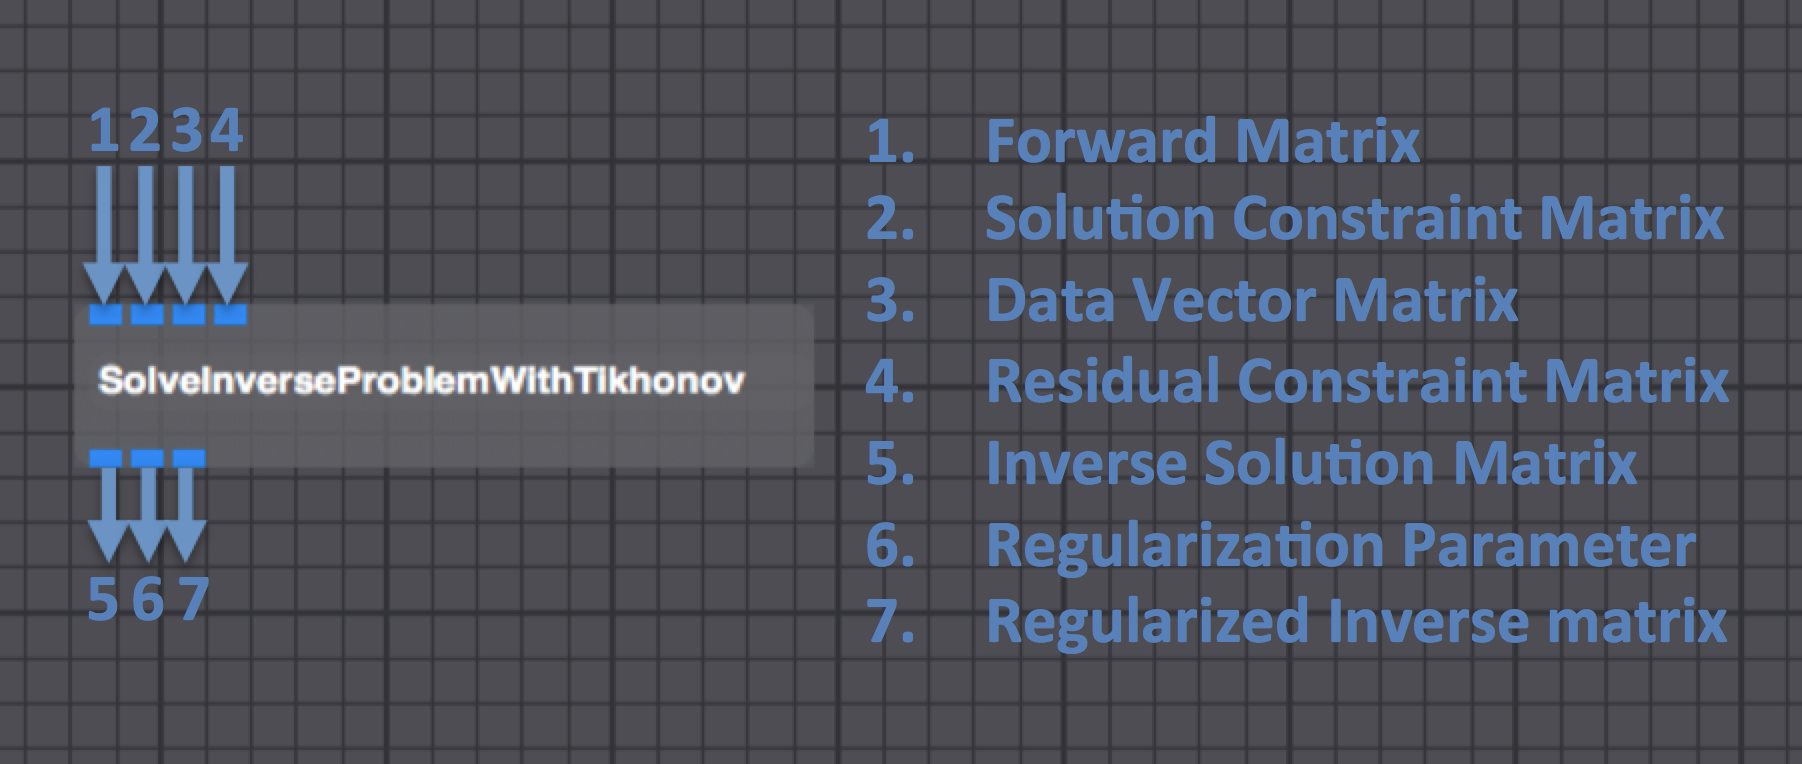
\includegraphics[width=0.7\textwidth]{ECGToolkitGuide_figures/tik1.png}
\caption{Revised Tikhonov module: {\tt SolveInverseProblemWithTikhonov}.  }
\label{tik_module}
\end{center}
\end{figure}

The module that solves the inverse problem by means of Tikhonov regularization is\\
\href{http://scirundocwiki.sci.utah.edu/SCIRunDocs/index.php/CIBC:Documentation:SCIRun:Reference:BioPSE:SolveInverseProblemWithTikhonov}{{\tt SolveInverseProblemWithTikhonov}}.
This module requires the Forward matrix and a vector of measured potentials (see figure \ref{tik_module}-1,3 ). In this case the module will calculate the standard Tikhonov regularization with $l2$ regularization:
\begin{center}
 \begin{eqnarray}
  x = argmin_x \|Ax -y\|_2 + \lambda \|x\|_2
 \end{eqnarray}
\end{center}

Optionally, the algorithm allows to use other constraints in both the solution and the measurements. In the module, this matrices are respectively called solution constraint 
matrix (R) and residual constraint matrix (L) (see figure \ref{tik_module}-2,4). In the general case the formula would result:
\begin{center}
 \begin{eqnarray}
  x = argmin_x \|Ax -Ly\|_2 + \lambda \|Rx\|_2
 \end{eqnarray}
\end{center}

The module is also prepared to compute the solution more efficiently depending in whether the problem is underdetermined or overdetermined. In both cases the underlying 
algorithm will be the Gaussian elimination, but the equations to solve will differ. This will give for the underdetermined case:
\begin{center}
 \begin{eqnarray}
  (ALL^TA^T + \lambda RR^T)x' &=& y\\
  x &=& LL^TA^Tx'
  \label{tik_problem_underdet_invop}
 \end{eqnarray}
\end{center}
\noindent and for the overdetermined case:
\begin{center}
 \begin{eqnarray}
  (A^TL^TLA + \lambda R^TR)x = A^TL^TLy 
  \label{tik_problem_overdet_invop}
 \end{eqnarray}
\end{center}

\noindent In both cases, the algorithm could be solved by using a linear operator $G$. This operator requires some inverses and might result in an inefficient implementation. 
For this reason it is not used as is, but it might be obtained by the user as one of the outputs of the module.\\
In the case of the overdetermined case the operator is:
\begin{center}
\begin{eqnarray}
   G &=& (A^{T} P^{T} P A + \lambda^{2} L L^{T})^{-1} A^{T} P^{T} P
\label{tik_problem_overdet_invop}
\end{eqnarray}
\end{center}
\noindent and for the underdetermined case:
\begin{center}
\begin{eqnarray}
   G &=& W W ^{T} A^{T} (A W W^{T} A^{T} + \lambda^{2} C C^{T})^{-1} .
\label{tik_problem_underdet_invop}
\end{eqnarray}
\end{center}


\begin{figure}[H]
\begin{center}
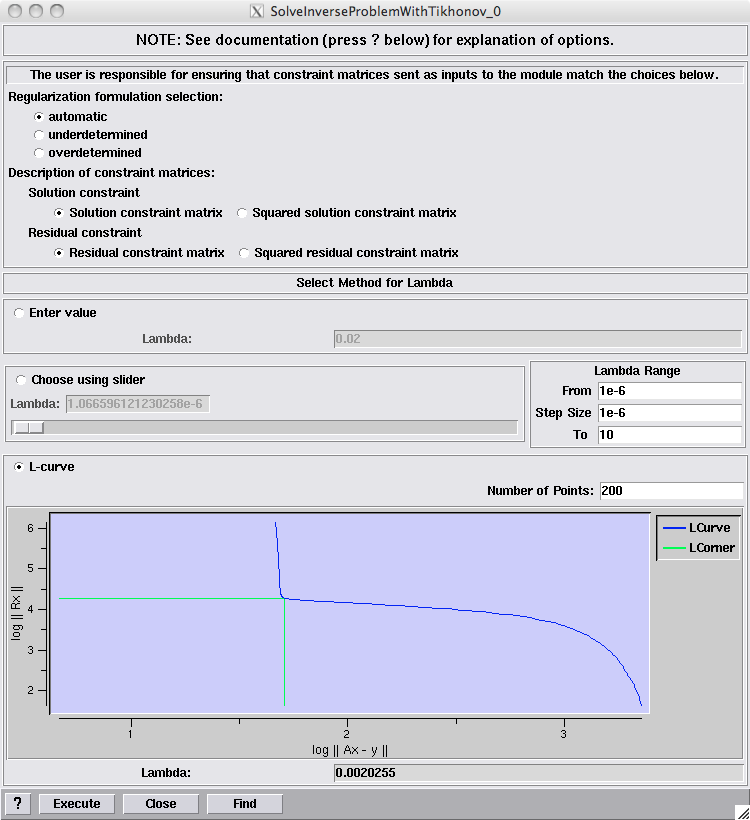
\includegraphics[width=0.8\textwidth]{ECGToolkitGuide_figures/tik2.png}
\caption{GUI from revised Tikhonov module: {\tt SolveInverseProblemWithTikhonov}.}
\label{tik_module_gui}
\end{center}
\end{figure}

\subsection*{Manual selection of the regularization parameter ``$\lambda$''}

The user is able to enter a specific regularization parameter to be used in
the inverse calculation. Further, the user can also specify a
range of equally distributed regularization parameters and select a particular one using the slider.

\subsection*{Automatic selection of the regularization parameter ``$\lambda$'' - the L-curve}

In figure \ref{tik_module_gui}, an example of a L-Curve is shown.
The automatic procedure to find the L-Curve corner evaluates the
curvature at each of the discrete points of the L-curve and estimates the maximal absolute curvature.

%% TODO: restore this text when the GUI has been rewritten in Qt, and there is a way to
%% pick a better regularization parameter
%Initially, the automatic procedure to find the L-Curve corner evaluates the
%curvature at each of the discrete points of the L-curve and estimates the maximal absolute curvature.
%In some cases, the automatically chosen regularization parameter is not optimal.
%Because of this, a slider under the L-Curve is available; it allows the user to choose a better regularization parameter.
%While moving the slider, the chosen L-Curve-Corner depicted in green, is updated.
%If a more reasonable regularization parameter is found by the user, it can be used later on for a single inverse computation
%by pressing the button, ``Update Lambda Value''.
%This will load the lambda value in the uppermost input field, which can later be activated with the radio button next to it.

\subsection*{Computational efficiency}

The module can automatically (by default) decide which case (overdetermined or
underdetermined) should be used to benefit from the most computationally efficient
approach. The user can manually decide which case should be used as
well (clicking to one of the radio buttons under ``Regularization formulation selection'').\\
%For demanding computations of the L-curve, the faster numerical
%approximation approach is used (formula \ref{tik_problem_overdet} or \ref{tik_problem_underdet})
%to determine the finally used regularization parameter. Any final solution is computed by
%using the more accurate inverse operator (see formula \ref{tik_problem_overdet_invop} and
%\ref{tik_problem_underdet_invop}). \\

To start any computation, the ``Execute'' button must be clicked.

%%%%%%%%%%%%%%%%%%%%%%%
\subsection{Tikhonov Singular Value Decomposition (SVD)}

\begin{figure}[H]
\begin{center}
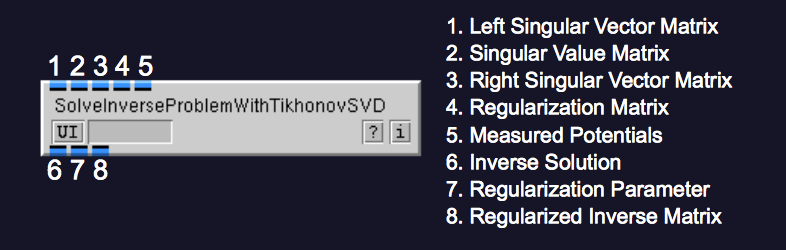
\includegraphics[width=\textwidth]{ECGToolkitGuide_figures/SolveInverseProblemWithTikhonovSVD.png}
\caption{Tikhonov SVD Module.}
\label{tikhonovsvd}
\end{center}
\end{figure}

\vspace{5pt}\textit{This is a method of solving the potential-based inverse problem.}\vspace{5pt}

This module implements Tikhonov regularization (closed-form solution) using the singular value decomposition (SVD) in SCIRun, and is called
\\{\tt SolveInverseProblemWithTikhonovSVD}. The module requires that the SVD of a forward solution matrix (left/right singular vector matrices and singular value matrix), regularization matrix (such as a surface Laplacian approximation), and a vector (single-column matrix) of observed/measured body surface potentials are supplied as input.

In the user interface (UI), one can explicitly specify a scalar regularization parameter that weights the influence of the regularization matrix on the solution. The module can also automatically select a regularization parameter using the L-curve method.

Upon completion, the module will output the inverse solution. In addition, it will either output the specified or automatically-chosen regularization parameter, as well as the regularized inverse matrix (a closed-form Tikhonov inverse operator, computed using the provided SVD).

%%%%%%%%%%%%%%%%%%%%%%%
\subsection{Truncated SVD}

\begin{figure}[H]
\begin{center}
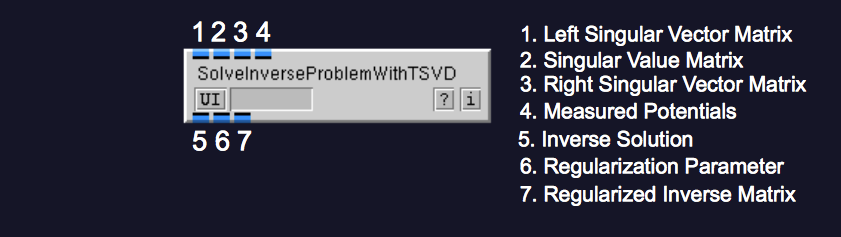
\includegraphics[width=\textwidth]{ECGToolkitGuide_figures/SolveInverseProblemWithTSVD.png}
\caption{Truncated SVD Module}
\label{tsvd}
\end{center}
\end{figure}

\vspace{5pt}\textit{This is a method of solving the potential-based inverse problem.}\vspace{5pt}

This module, called {\tt SolveInverseProblemWithTSVD}, computes an inverse solution by creating a pseudo-inverse operator and multiplying that with the measured body surface potentials. The module requires that the SVD of a forward solution matrix (left/right singular vector matrices and singular value matrix) and a vector of observed/measured body surface potentials are supplied as input.

In the user interface (UI), one can explicitly specify a scalar-integer regularization parameter to control the amount of regularization imposed on the problem. Assuming the singular values are sorted from largest to smallest (and therefore most significant to least significant), the regularization parameter controls how many significant singular values to consider (truncation degree) when calculating the pseudo-inverse. Alternatively, the module will use the L-curve method to automatically obtain a suitable truncation degree.

The primary output of this module is a vector containing the inverse solution. In addition, it will output the regularization parameter and regularized inverse operator used to obtain the inverse solution from the measured body surface potentials.

%%%%%%%%%%%%%%%%%%%%%%%%%

\subsection{Matlab Interface}

The \textit{InterfaceWithMatlab} module allows a SCIRun network to make use of Matlab for some of its calculations. In Figure \ref{matlabinterfacemodule}, the user interface for this module shows how SCIRun data types from the module's input pipes are converted to Matlab variables for use in a Matlab script. Upon completion of the Matlab script, Matlab variables are converted back to SCIRun data types to be sent to the module's output pipes.

\begin{figure}[H]
\begin{center}
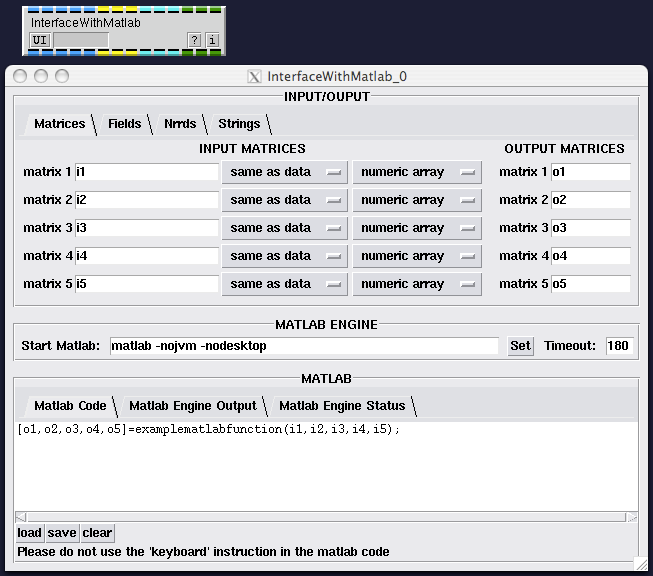
\includegraphics[width=0.8\textwidth]{ECGToolkitGuide_figures/InterfaceWithMatlab.png}
\caption{The InterfaceWithMatlab Module and its corresponding user interface}
\label{matlabinterfacemodule}
\end{center}
\end{figure}

In the rest of this section, we will describe some of the inverse solution methods distributed with SCIRun that have been implemented in Matlab.


\subsubsection{Isotropy Method}

\vspace{5pt}\textit{This is a method of solving the potential-based inverse problem.}\vspace{5pt}

\begin{verbatim}
function X_reg=greensite(A,Y,trunc_deg)
% Function to calculate the Greensite inverse solution
%   A - forward matrix
%   Y - data
%   trunc_deg - truncation degree
%   X_reg - inverse solution
\end{verbatim}

The isotropy method (a.k.a. Greensite method) takes as input a forward solution matrix, measured body surface potential data, and an optional integer regularization parameter (truncation degree). In this method, the truncation degree controls the number of significant singular values of the measured body surface potential data to be used when computing the inverse solution. Consequently, the truncation degree partitions the measured body surface potential data into independent ``signal'' and ``noise'' components, ignoring the ``noise'' component in its calculation of the inverse solution. The only output of the method is the inverse solution.

\subsubsection{Gauss-Newton Method}

\vspace{5pt}\textit{This is a method of solving the activation-based inverse problem.}\vspace{5pt}

\begin{verbatim}
function tau = ActGaussNewton(A,Y,L,tauinit,lambda,w,minstep)
% Implements the Gauss-Newton algorithm for solving the activation-based
% inverse problem of electrocardiography.
% => minimizes the objective function ||Y-A*X||^2+lambda*||L*X||^2 where
% X is parameterized by the C^1 polynomial approximation to a step function
% as explained in "The Depolarization Sequence of the Human Heart Surface
% Computed from Measured Body Surface Potentials" by Geertjan Huiskamp and
% Adriaan van Oosterom.
%
% Input Variables:
% A: Forward matrix
% Y: Observations (columns index time from 1 to T=size(Y,2))
% L: Regularization matrix (typically a surface Laplacian approximation)
% lambda: Regularization parameter
% w: Width parameter in step function approximation
% tauinit: Initial phase shifts for starting the algorithm
%
% Output Variables:
% tau: Solution phase shifts of the step functions
\end{verbatim}

The activation-based inverse problem of electrocardiography is to solve for electrical activation times (i.e. depolarization times) on the heart, given body surface potentials during the QRS complex. This results in a nonlinear least-squares optimization problem that this method solves using the Gauss-Newton algorithm. Solutions are typically highly dependent on the choice of the initial guess. This method requires a forward solution matrix, body surface potentials, regularization matrix, initial guess, regularization parameter, activation waveform transition width, and convergence parameter to be specified as input. The body surface potentials should be provided as a $M \times T$ matrix, where $M$ is the number of leads from which potentials are recorded and $T$ is the number of time samples recorded during the QRS complex of the heart, whose activation times are to be estimated. The regularization matrix and corresponding parameter influence the inverse solution as in Tikhonov regularization (see above). The initial guess is the set of activation times from which the Gauss-Newton algorithm starts pursuing a more suitable inverse solution. The transition width controls the number of time samples (not necessarily integer) taken by each source to transition from inactivated to activated in this method. The convergence parameter is the minimum norm of the step taken by the iterations within the Gauss-Newton algorithm before the method is deemed to have converged to a suitable solution. The only output of the method is the inverse solution (in this case: an array/vector of activation times).

\subsubsection{Wavefront-Based Potential Reconstruction}

\vspace{5pt}\textit{This is a method of solving the potential-based inverse problem.}\vspace{5pt}

\begin{verbatim}
function [x_WBPR_forward,x_WBPR_backward] = WBPR(A,y,heart,first_act,last_act)
% Function to calculate the WBPR solutions
% Inputs:
%   A: forward matrix
%   y: torso data
%   heart: heart geometry
%   first_act: first activated node
%   last_act: last activated node
%
% Outputs:
%   x_WBPR_forward: inverse solution using forward WBPR
%   x_WBPR_backward: inverse solution using backward WBPR
\end{verbatim}

The Wavefront-Based Potential Reconstruction (WBPR) method imposes prior knowledge about the spatial patterns of electric potentials on the heart during the QRS complex to reconstruct an inverse solution. This method requires a forward solution matrix, measured body surface potentials, a structure containing the triangles and nodes of the heart geometry mesh, and the first/last nodes to activate during the QRS complex of the heart beat. The body surface potentials should be provided as a $M \times T$ matrix, where $M$ is the number of leads from which potentials are recorded, and $T$ is the number of time samples recorded during the QRS complex of the heart beat, whose electric potentials are to be estimated. The heart geometry is a Matlab ``struct'' that must contain a matrix of node coordinates and a matrix of indices for triangles that connect the nodes on the surface of the heart. The first/last nodes to activate are specified as the indices of the nodes.

As output, WBPR produces two inverse solutions. The procedure by which the inverse solutions are obtained may be run both forward and backward in time. Therefore, the ``forward WBPR'' solution is that obtained by applying the method starting from the earliest sample time and ending at the latest. On the other hand, the ``backward WBPR'' solution is obtained by starting from the latest sample time and traversing the samples in reverse until ending at the earliest.

NOTE: This code requires the software package reguTools (http://www.imm.dtu.dk/~pcha/Regutools/) to be incorporated in the default path from MATLAB.


\subsubsection{Non-Negative Transmembrane Potential Inverse}

\vspace{5pt}\textit{This is a method of solving the potential-based inverse problem.}\vspace{5pt}
\begin{verbatim}
%% MESSNARZ INVERSE SCRIPT FOR SCIRUN
%
%		This is a script for the matlab interface in the SCIRUN network
%		nonNegative.srn.
%		This method consists in a potential based inverse method that 
%		uses tikhonov reularization in a minimization algorithm that 
%		constrains the solutions to be monotonically non-decreasing.
%		
%			Inputs:
%				   i1 - double - primal/dual tradeoff parameter from the ADMM algorithm.
%				   i2 - <N,T>double - ECG recordings. (N leads, T time samples)
%				   i3 - <N,M>double - forward matrix.
%				   i4 - <1,3>int - lambda parameters: [minLam maxLam numLam].
%			                           minLam - minimum lambda = 10^minLam
%			                           maxLam - maximum lambda = 10^maxLam
%			                           numLam - number of lambdas to use 
%			Outputs::
%				   o1 - <M,T>double - estimated solution.
%				   o2 - <M,T+1>double - dual variables of ADMM code.
%
\end{verbatim}

The non-negativeTMP code estimates the transmembrane potentials by solving a constrained Tikhonov problem.
Thus the function to be optimized over is a standard Tikhonov problem but restricts the solutions to always be non-decreasing.
Thus, the problem to be solved is:
\begin{equation}\begin{split}
		\min_{x(t), t=1\dots T} &\|y(t) - Ax(t)\|_2^2 + \lambda*\|Rx(t)\|_2^2 \\
		&s.t.\\
   		&\hspace{2cm}x(1) >= minB\\
     	&\hspace{2cm}x(t+1) >= x(t), \hspace{.2cm}t=1\dots T-1\\
     	&\hspace{2cm}x(T) <= maxB
\end{split}
\end{equation}
Where $minB$ and $maxB$ are the minimum and maximum bounds for the TMP.
For memory efficiency, this problem is implemented with an ADMM solver.
This algorithm tends to work well for relatively small geometries ($<1000$ nodes).
The resulting potentials have sharp increases of potentials similar to the typically observed in TMPs 
for most of the nodes on the heart geometry.
In general, the final solution is insensitive to the initial guess but it will affect the time of convergence.
The script is set up such that the initial guess for the first lambda is a simple ramp, after each initial guess is the final result of the previous lambda. 
The decision of the correct lambda is done automatically using an L-corner detection.
This algorithm is implemented as the SCIRUN network nonNegativeTMP.srn

NOTE: This code requires the software package reguTools (http://www.imm.dtu.dk/~pcha/Regutools/) to be incorporated in the default path from MATLAB.

\subsubsection{Spline Interpolation Inverse}

\vspace{5pt}\textit{This is a method of solving the potential-based inverse problem.}\vspace{5pt}
\begin{verbatim}
%		This code implements the inverse solutions pipeline presented in
%		the paper:
%	        Erem, Coll-font, Martinez Orellana - 2013 - 
%	        Using Transmural Regularization and Dynamic Modeling 
%	        for Non-Invasive Cardiac Potential Imaging of 
%	        Endocardial Pacing Sites with Imprecise Thoracic Geometry.
%
%		Inputs
%				  i1 - <N,T>double - measured potentials on the torso.
%				  i2 - <N,M>double - forward matrix.
%				  i3 - <L,M>double - regularization matrix.
%				  i4 - <3,1>int - regularization constant params.
%				                  i4(1) - log10 min lambda.
%				                  i4(2) - log10 max lambda
%				                  i4(3) - num lambda.
%		Outputs
%				  o1 - <M,T>double - estimated heart potentials.
\end{verbatim}

This code implements a spline interpolation based inverse for ECG.
It works under the assumption that the measured cardiac potentials, treated as a vector in high dimensional space, span a 1-D manifold in time.
This algorithm approximates this manifold with a spline, effectively filtering out noise to describe the evolution of these potentials.
Then it estimates the inverse of the reference points (knot points) of the spline and reconstructs the full evolution of potentials in the heart using the time dynamics from the body surface potentials.
This algorithm works well when the regularization matrix used in the inverses estimates the spatial derivative in the volume of the heart.
An example of a SCIRUN implementation for this code can be found in the spline$\_$inverse.srn network. 

\subsubsection{Total Variation Inverse}

\vspace{5pt}\textit{This is a method of solving the potential-based inverse problem.}\vspace{5pt}
\begin{verbatim}
%	This script implements a Total Variation method to solve the inverse
%	problem in electrocardiography 
%
%	This code needs of the convex optimization toolbox from CVX
%	(http://cvxr.com/cvx/)
%
%	Inputs:
%    field1 - struct - full bofy geometry.
%    field2 - struct - heart geometry.
%    field3 - struct - torso geometry.
%    i1 - <N,1>double - ECG measured potentials.
%     i2 - <N,1>int - indices of the geometry where ECG where measured.
%    i3 - <M,M>double - stiffness matrix on the heart.
%     i4 - <N+M,N+M>double - stiffness matrix on the whole body.
%	Outputs:
%    o1 - <M,1>double - estimated inverse solution.
%
%	Dependencies:
%    cvx - convex optimization package
%
\end{verbatim}

This code is an implementation of a full pipeline that covers from the solution of the forward problem to an implementation of a Total Variation inverse solution.
This method uses a FEM geometry to calculate the forward matrices needed and then computes the inverse solution from body surface measurements.
The solutions it obtains tend to have sharper spatial transitions that the regular Tikhonov solutions.
An example SCIRUN implementation for this MATLAB implementation is the Total$\_$Variation.srn in the FwdInvToolbox.

NOTE: This code requires the software package CVX (http://cvxr.com/cvx/) for MATLAB to be set up in the default path of MATLAB.

%%%%%%%%%%%%%%%%%%%%%%%%%
\section{Example Simulations}

\subsection{Tikhonov Regularization}

\vspace{5pt}\textit{The SCIRun network for this example can be found at:\\{\tt src/nets/FwdInvToolbox/potential-based-inverse/tikhonov-inversion.srn}\\in the SCIRun source code directory.}\vspace{5pt}

\begin{figure}[H]
\begin{center}
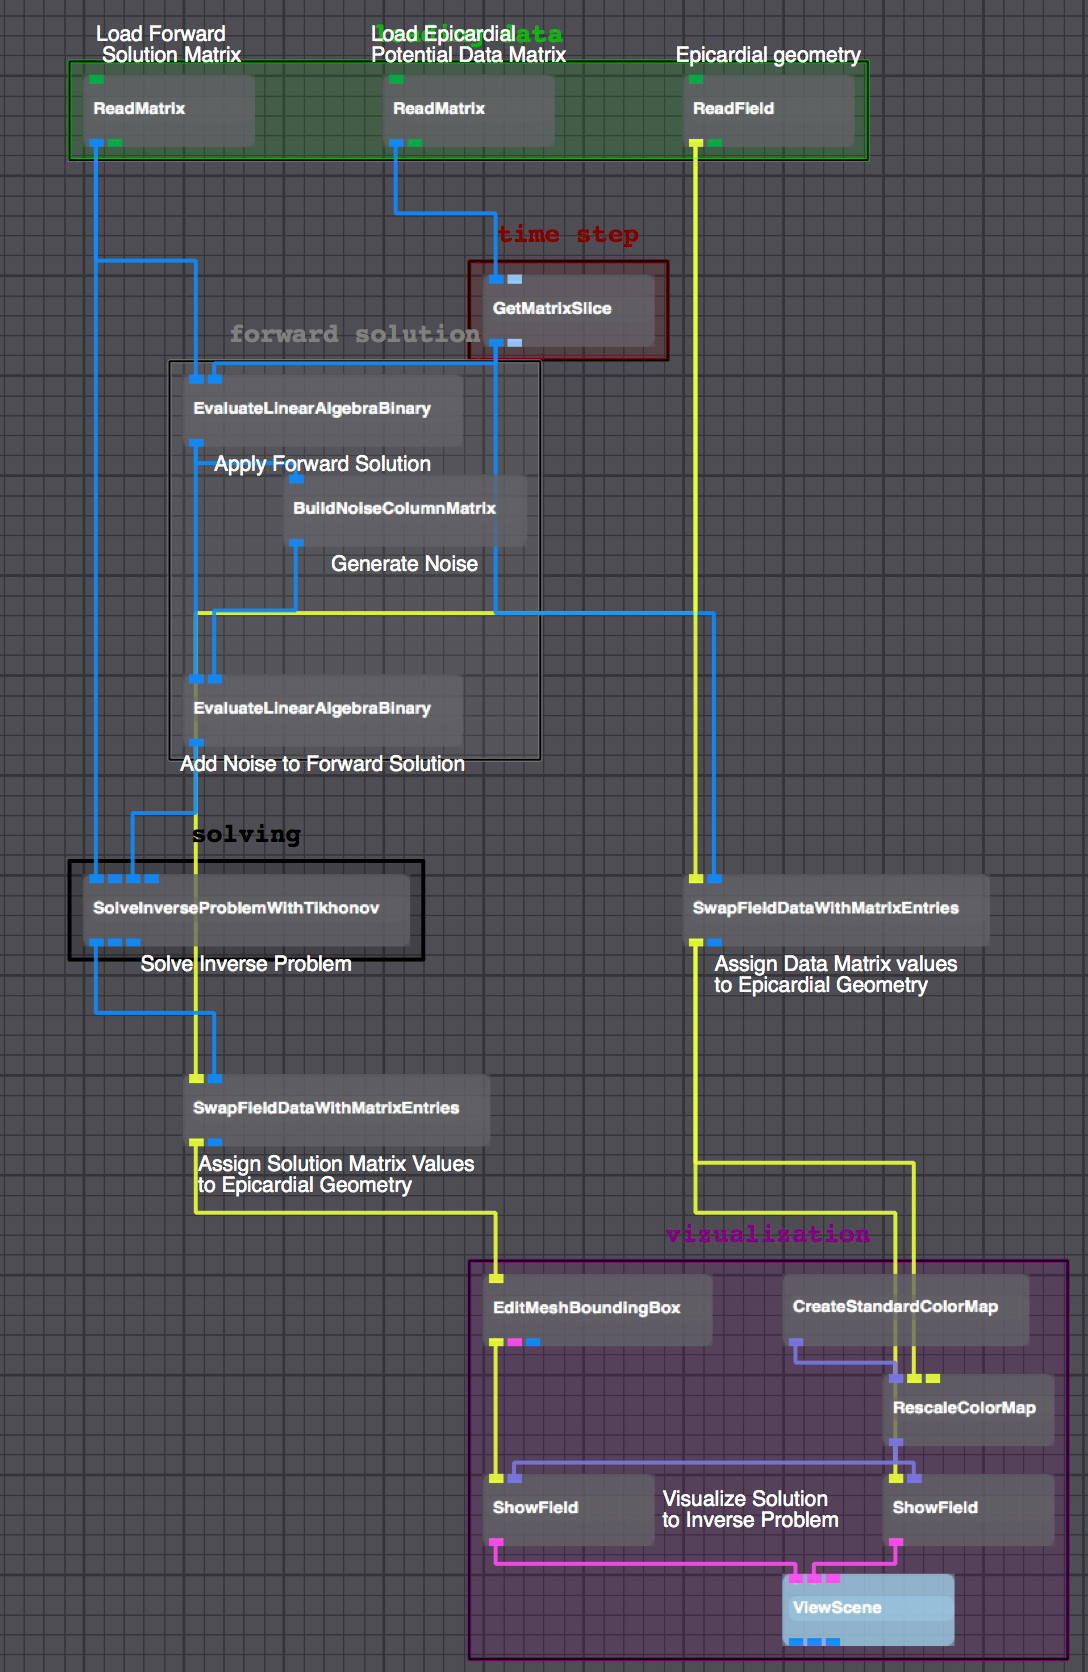
\includegraphics[width=0.9\textwidth]{ECGToolkitGuide_figures/TikhonovNetwork.png}
\caption{The SCIRun network for the Tikhonov inverse solution example.}
\label{TikhonovNetworkExample}
\end{center}
\end{figure}

This example shows how to use the {\tt SolveInverseProblemWithTikhonov} module in a SCIRun network to solve a potential-based ECG inverse problem using Tikhonov regularization. Specifically, this example simulates ``measured'' body surface potentials by applying a forward solution and adding pseudorandom noise with a specified signal-to-noise ratio (SNR). The forward solution is obtained by multiplying a known vector of epicardial potential data by a pre-computed forward solution matrix. The simulated measurements and forward solution matrix are the inputs to the {\tt SolveInverseProblemWithTikhonov} module. The regularization parameter of this method is controlled via the user interface (UI) in this example. The output from the module is the inverse solution. This example compares the inverse solution to the known epicardial potentials from which the measurements were simulated. A visualization of both can be seen in the UI of the {\tt ViewScene} module.

\subsection{Gauss-Newton Method}

\vspace{5pt}\textit{The SCIRun network for this example can be found at:\\{\tt src/nets/FwdInvToolbox/activation-based-inverse/actgaussnewton-inversion.srn}\\in the SCIRun source code directory.}\vspace{5pt}

This example shows how to use the {\tt InterfaceWithMatlab} module in a SCIRun network to solve an activation-based ECG inverse problem using the Gauss-Newton method. This example uses the ``normal male'' dataset and geometries from ECGSIM. Specifically, this method compares measured body surface potentials with body surface potentials simulated from activation times. We search the set of possible activation times for ones that minimize the squared error residual between the measured and simulated body surface potentials. The Gauss-Newton method in this example is implemented as a Matlab function and is used in SCIRun via the {\tt InterfaceWithMatlab} module. As a numerical optimization method, Gauss-Newton will look for a local minimizer of the squared error residual starting from a suitable initialization point. In this example, we initialize the method with the activation times reported for the dataset in ECGSIM, but perturbed by noise.

\begin{figure}[H]
\begin{center}
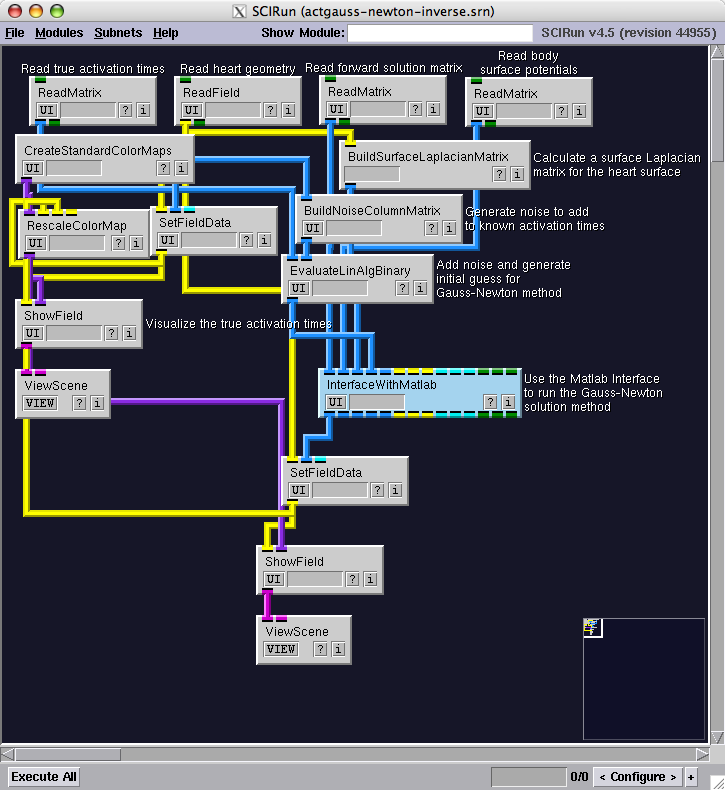
\includegraphics[width=0.9\textwidth]{ECGToolkitGuide_figures/actgaussnewtonnetwork.png}
\caption{The SCIRun network for the activation-based Gauss-Newton inverse solution example.}
\label{GaussNewtonNetworkExample}
\end{center}
\end{figure}





\end{document}

